\documentclass[justified,nobib,symmetric,twoside]{tufte-handout}

\title[Empirische Studien zu Fragen der Bedarfsgerechtigkeit]{Empirische Studien\\zu Fragen der Bedarfsgerechtigkeit}
\author[Alexander Max Bauer]{\upshape Alexander Max Bauer}
\date{}

\usepackage[utf8]{inputenc}

\usepackage{amsmath}
\usepackage{amssymb}
\usepackage[ngerman]{babel}
\usepackage[backend=biber,maxnames=3,maxbibnames=99,natbib=true,style=ext-authoryear-comp,dashed=false,uniquelist=false]{biblatex}
   \addbibresource{references.bib}
   \DefineBibliographyStrings{ngerman}{andothers={{et\,al\adddot}}}
   \renewcommand*{\nameyeardelim}{\space}
   \renewcommand*{\multicitedelim}{\addcomma\space}
\usepackage{booktabs}
\usepackage[autostyle,german=guillemets]{csquotes}
\usepackage{ebgaramond}
\usepackage{fancyvrb}
   \fvset{fontsize=\normalsize}
\usepackage{graphicx}
   \setkeys{Gin}{width=\linewidth,totalheight=\textheight,keepaspectratio}
   \graphicspath{{figures/}}
\usepackage{microtype}
\usepackage{nameref}
\usepackage[defaultlines=2,all]{nowidow}
\usepackage{pdfpages}
\usepackage{url}
   \urlstyle{same}
\usepackage{xargs}
\usepackage{xspace}

\setcounter{secnumdepth}{2}
\setcounter{tocdepth}{1}

\addto\captionsngerman{
  \renewcommand{\contentsname}
    {Inhalt}
}

\begin{document}


%%%%%%%%%%%
% TITELEI %
%%%%%%%%%%%
\begin{titlepage}
   \begin{center}
      \vspace*{3cm}
      {\Huge\textsc{Empirische Studien zu}}
      
      \vspace*{0.3cm}
      {\Huge\textsc{Fragen der}}
      
      \vspace*{0.3cm}
      {\Huge\textsc{Bedarfsgerechtigkeit}}
   \end{center}
   \vfill
   {\Large\noindent Von der Carl von Ossietzky Universität Oldenburg -- Fakultät IV, Human- und Gesellschafts­wissenschaften -- zur Erlangung des Grades eines}
   
   \vspace{0.4cm}
   {\Large Doctor philosophiae (Dr.\,phil.)}
   
   \vspace{0.4cm}
   {\Large\noindent genehmigte Dissertation}
   
   \vspace{0.4cm}
   {\Large von Herrn Alexander Max Bauer,}
   
   {\Large geboren am 12. Dezember 1989 in Böblingen}
\vfill
\end{titlepage}

\clearpage
\begin{titlepage}
   \null
   \vfill
   {\Large\textsc{Referent:}\hspace{1cm}Prof. Dr. phil. Mark Siebel}

   \vspace{0.3cm}
   {\Large\textsc{Korreferent:}\hspace{0.23cm}}

   \vspace{1cm}
   {\Large\textsc{Tag der Disputation:}}
\end{titlepage}


%%%%%%%%%
% TITEL %
%%%%%%%%%
\clearpage
\setcounter{page}{1}
\maketitle


%%%%%%%%%%%%
% ABSTRACT %
%%%%%%%%%%%%
\begin{abstract}
   \noindent In dieser Dissertation wird mittels einer Reihe von Vignettenstudien untersucht, welche Rolle Bedürfnisse im Umgang mit Problemen der Verteilungsgerechtigkeit spielen.
   Sie enthält dabei, unter anderem, sieben Hauptergebnisse:
   (1) In der Rolle von unparteiischen Beobachter*innen nehmen Versuchsteilnehmer*innen graduelle Gerechtigkeitseinschätzungen von Verteilungssituationen vor.
   (2) Diese Einschätzungen sind abhängig davon, wie umfangreich die beobachteten Parteien mit einem Gut ausgestattet sind.
   (3) Wenn außerdem bekannt ist, wie hoch deren Bedarf an jenem Gut ist, finden die Einschätzungen relativ zu diesem Referenzpunkt statt.
   (4) In der Rolle von unparteiischen Entscheider*innen treffen Versuchsteilnehmer*innen hypothetische Verteilungsentscheidungen, die den Bedarf, die Leistung sowie die Verantwortung der betroffenen Parteien berücksichtigen.
   (5) Hierbei wird der Bedarf einer Partei auch dann zumindest teilweise kompensiert, wenn diese weniger zu der zur Verfügung stehenden Gütermenge beigetragen hat, als sie selbst benötigt.
   (6) Die Bereitschaft, den Bedarf einer Partei teilweise zu kompensieren, sinkt jedoch, wenn sie dafür verantwortlich ist, mehr als andere zu benötigen oder weniger als andere beigetragen zu haben.
   (7) Sowohl in der Rolle von unparteiischen Beobachter*innen als auch in der Rolle von unparteiischen Entscheider*innen unterscheiden Versuchsteilnehmer*innen zwischen unterschiedlichen Bedarfsarten, deren Erfüllung sie verschiedene Wichtigkeit beimessen.
\end{abstract}


%%%%%%%%%%
% INHALT %
%%%%%%%%%%
\vspace{1em}
\tableofcontents
\clearpage


%%%%%%%%%%%%%%
% EINLEITUNG %
%%%%%%%%%%%%%%
\section{Einleitung}\label{sec:einleitung}
Die vorliegende Arbeit verstehe ich als einen Beitrag zur deskriptiven Ethik.
Die deskriptive Ethik rechne ich~-- in meinem breiten Verständnis derselben~-- zur Experimentellen Philosophie.
Und die Experimentelle Philosophie ihrerseits sehe ich~-- wiederum in meinem breiten Verständnis derselben~-- als einen Teil der Philosophie im Ganzen.
Obgleich die Experimentelle Philosophie die Philosophie selbst im Namen trägt, ist dieser letzte Punkt bei Weitem nicht unumstritten: Mithin wird gefragt, ob sich überhaupt von Philosophie sprechen lasse, wenn mit empirischen Methoden gearbeitet wird.
Meine grundlegende Perspektive hierauf habe ich bereits an anderer Stelle dargelegt \citep{bauer_was_2020_a,bauer_was_2020_b}.
Den Platz hier möchte ich dagegen nutzen, um kurz darzustellen, auf welche Weise deskriptive Ethik auch für normative Ethik relevant werden kann.

\citet[S.~177ff.]{miller_review_1994} unterscheidet prominenterweise zwei Grundpositionen, wenn es um die Frage geht, ob empirische Forschung etwas zur normativen Ethik beizutragen habe.
Er spricht von einer \enquote{platonischen} Perspektive, wenn diese Frage verneint wird, und einer \enquote{aristotelischen} Perspektive, wenn sie demgegenüber bejaht wird.
Letztere ist vor dem Hintergrund dieser Arbeit besonders interessant.
Aus welchen Gründen lässt sich davon ausgehen, dass deskriptive Ethik und die durch sie gewonnenen empirischen Daten für normative Ethik relevant sein können?
Hier möchte ich nur drei exemplarische Thesen in aller Knappheit vorstellen.\footnote{Diese Überlegungen sind zusammengefasst in \citet{bauer_zwei_2019,bauer_two_2020}.}

Erstens: Empirische Daten können, wie es \citet{bar-hillel_judgments_1993} ausgedrückt haben, für einen Prozess der Selbstkorrektur von Bedeutung sein.
Normative ethische Theorien werden in der Regel vor dem Hintergrund der eigenen Intuitionen konstruiert; allenfalls fließen hier noch Intuitionen der Korrespondenzpartner oder Vordenker ein.
Im Rahmen der deskriptiven Ethik können systematisch weitere Einstellungen zu relevanten Fragen ermittelt werden.
\enquote{Hier kann durch empirische Daten quasi die Grundgesamtheit der Introspektionen erweitert werden, über die reflektiert wird} \citep[S.~21]{bauer_zwei_2019}.
Miller zeigt mit Blick auf \citet{rawls_theory_1971}, warum das wichtig ist.
Seinen Gedanken fasst \citet[S.~11]{honneth_philosophie_2008} prägnant zusammen:

\begin{quote}
   Weil Rawls alle Untersuchungen zu alltäglichen Gerechtigkeitsempfindungen zur Seite schiebt, ja, weil er sie nicht einmal prüfend zur Kenntnis nimmt, lässt er sich wider allen Augenschein dazu hinreißen, die soziale Gerechtigkeit im Ganzen auf den einen Wert der Gleichheit zu gründen; hätte er hingegen derartige Studien vorweg zu Rate gezogen, so möchte Miller sagen, dann wäre Rawls schnell zu der Einsicht gelangt, dass die von ihm beschworene Bürgerschaft mehr als nur ein Gerechtigkeitsprinzip für nötig und für gerechtfertigt hält.
\end{quote}

Zweitens: Normative ethische Theorien kommen in aller Regel nicht ohne Bezug zur empirischen Welt aus, da es menschliche Verhältnisse sind, die sie in den Blick nehmen, und diese Verhältnisse nun einmal Teil der empirischen Welt sind.
Solche Theorien beinhalten in der Folge häufig Prämissen mit Aussagen über jene Welt.
Sie sind damit~-- in diesen Teilen~-- prinzipiell auch durch die Ergebnisse empirischer Forschung falsifizier- oder stützbar, was weitreichende Konsequenzen haben kann.
Ganz in diesem Sinne hat beispielsweise \citet[S.~670]{kutschera_empirische_1988} festgestellt: \enquote{Lässt sich etwa das Menschenbild nicht aufrechterhalten, das unsere ethischen Maximen voraussetzen, so sind auch diese zu revidieren.}

Drittens: Normative ethische Theorien werden in aller Regel mit dem Ziel formuliert, \enquote{schließlich in Praxis zu münden} \citep[S.~22]{bauer_zwei_2019}.
Hier kann empirische Forschung in zweierlei Hinsicht von Bedeutung sein.
Aus einer Ex-ante-Perspektive lassen sich beispielsweise mögliche Diskrepanzen zu vorherrschenden Moralvorstellungen oder mögliche konzeptuelle Missverständnisse identifizieren, die dann adressiert werden können.
Aus einer Ex-post-Perspektive wiederum kann außerdem untersucht werden, ob mit der Befolgung einer gewissen Theorie tatsächlich die durch sie intendierten Zwecke erreicht wurden, sofern diese Zwecke denn messbarer Natur sind.

Es zeigt sich, dass mit keiner dieser Thesen von einem naiven Gerechtigkeitspositivismus ausgegangen werden soll, dass aber~-- mit David Miller gesprochen~-- eine \enquote{komplementäre Angewiesenheit von Sozialwissenschaften und politischer Philosophie, von empirischer Gerechtigkeitsforschung und normativer Gerechtigkeitstheorie} \citep[S.~10]{honneth_philosophie_2008} zu vermuten ist.
Ganz in diesem Sinne können auch die nachfolgend vorgestellten Ergebnisse für normative Ethik relevant werden.\footnote{Das Spannungsfeld zwischen deskriptiver und normativer Perspektive ist freilich ungleich komplexer, als hiermit angedeutet ist. Ausführlicher behandelt wird es unter anderem in \citet{appiah_experiments_2009}, \citet{bauer_philosophie_2019,bauer_empirical_2020}, \citet{christen_empirically_2014}, \citet{eckensberger_ethische_1993}, \citet{karageorgoudis_sein_2021}, \citet{luetge_experimental_2014}, \citet{marchetti_facts_2017}, \citet{paulo_empirische_2020} sowie \citet{poelzler_moral_2018}.}
Dieses Potential auszuloten, soll aber nicht im Fokus der vorliegenden Arbeit stehen; dieser soll vielmehr auf der deskriptive Perspektive liegen.

In Abschnitt~\ref{sec:gegenstand} wird zunächst in aller Kürze das begriffliche Feld abgesteckt, auf dem sich diese Arbeit bewegt, bevor in den Abschnitten~\ref{sec:referenzpunkt} bis~\ref{sec:bedarfsarten} die Ergebnisse empirischer Studien vorgestellt werden.
In Abschnitt~\ref{sec:referenzpunkt} geht es dabei zunächst um die Frage, ob es eine Verbindung gibt zwischen der Gerechtigkeitseinschätzung einer Situation und der in dieser Situation vorherrschenden Güterversorgung und Bedarfsdeckung.
In Abschnitt~\ref{sec:verantwortung} wird dann der Frage nachgegangen, ob neben solchen passiven Gerechtigkeitseinschätzungen auch aktive Verteilungsentscheidungen, die von unparteiischen Entscheider*innen für zwei hypothetische Personen getroffen werden, von Bedarfsinformationen beeinflusst werden.
In Abschnitt~\ref{sec:bedarfsarten} wird dann ein Blick darauf geworfen, welche Rolle unterschiedliche Bedarfsarten spielen, wenn Bedarfsarten entweder hinsichtlich ihrer Wichtigkeit bewertet werden (Abschnitt~\ref{sec:bedarfsarten_1}) oder bei der Verteilung eines Gutes auf zwei hypothetische Personen berücksichtigt werden müssen (Abschnitt~\ref{sec:bedarfsarten_2}).
Abschnitt~\ref{sec:zusammenfassung} schließlich fasst die zentralen Ergebnisse noch einmal zusammen.


%%%%%%%%%%%%%%
% GEGENSTAND %
%%%%%%%%%%%%%%
\section{Zum Gegenstand}\label{sec:gegenstand}
Diese Arbeit ist im Allgemeinen, Titel und Einleitung haben das schon angedeutet, mit Fragen der Gerechtigkeit befasst.
Im Speziellen ist sie dies im Rahmen der deskriptiven Ethik und mit einem besonderen Fokus auf Bedarfsgerechtigkeit.
Bevor ich nun auf die deskriptiven Befunden zu sprechen komme, soll hier knapp das begriffliche Feld abgesteckt werden, auf dem sich diese Arbeit bewegt.\footnote[][-0.1cm]{Weite Teile dieses Abschnitts beruhen auf \citet{bauer_gerechtigkeit_2019}, einer erweiterten Fassung des zweiten Kapitels meiner Masterarbeit (siehe auch \cite{bauer_monotonie_2018} und \cite{bauer_grundlegung_2019}).}

Wenn ich im Folgenden von \textit{Gerechtigkeit} spreche, dann habe ich dabei zunächst einmal folgenden formalen Gerechtigkeitsbegriff im Sinn: Gerechtigkeit im allerweitesten Sinne \enquote{meint das richtige Zueinander einzelner Teile eines Ganzen} (\cite[S.~289]{bauer_gerechtigkeit_2019}).
Das bleibt zunächst natürlich ähnlich dunkel wie das, was Platon in der \textit{Politeia} dem Simonides zugeschrieben hat: \enquote{So hat denn also, sagte ich, wie es scheint, Simonides nach Dichterart angedeutet, was das Gerechte sei: daß man jedem gebe, was ihm gebühre, und hat dies als Schuldigkeit bezeichnet} \citep[S.~13, 332\,b--\,c]{platon_staat_2004}.
Dieser formale Begriff macht deutlich, dass Gerechtigkeit ein fundamental relationales Konzept ist, er sagt aber nicht, was eigentlich gerecht ist.
Hierzu müsste diesem formalen Gerechtigkeitsbegriff ein materialer Begriff an die Seite gestellt werden.
Gerechtigkeitstheorien von Sokrates, Platon oder Aristoteles, von Immanuel Kant oder John Rawls, von Amartya Sen oder Martha Nussbaum verstehe ich als Versuche, einen solchen materialen Gerechtigkeitsbegriff auszubuchstabieren; sie versuchen zu ergründen, worin dieses richtige Zueinander besteht und wie es sich legitimieren lässt.

Zurückgehend auf eine aristotelische Unterscheidung \citep{aristoteles_nikomachische_2006}, engt die \textit{Verteilungsgerechtigkeit} das Feld nun auf die Frage ein, wie gewisse~-- nicht zwingend, aber im Folgenden doch durchgehend physische~-- Güter richtigerweise auf die Mitglieder einer Gruppe zu verteilen seien.
Hier ist im Laufe der Zeit eine Reihe von \textit{Verteilungsprinzipien} vorgeschlagen worden, die anzugeben versuchen, an welchen Merkmalen sich eine Verteilung in welcher Weise zu orientieren habe, um als gerecht gelten zu können.
Solche Prinzipien erscheinen häufig für sich genommen legitim, können aber, sobald sie nicht mehr isoliert betrachtet werden, miteinander konfligieren, wie \citet[S.~290f.]{sen_resources_1984} eindrücklich vorgeführt hat.
Man stelle sich dazu, Sen folgend, folgende Situation vor.
Drei Kinder kommen auf einen zu.
Sie haben eine Flöte bei sich und bitten darum, zu entscheiden, wer von ihnen sie bekommen solle.
Nun gibt es drei verschiedene Varianten dieser Geschichte.
In der ersten Variante erfährt man lediglich, dass eines der Kinder wesentlich musikalischer ist als die beiden anderen.
Wahrscheinlich würde es dementsprechend wesentlich mehr Nutzen aus der Flöte ziehen.
Utilitaristischen Überlegungen folgend könnte es in dieser Variante der Geschichte also legitim erscheinen, diesem Kind die Flöte zuzusprechen.
In der zweiten Variante erfährt man wiederum nur, dass es einem der Kinder wesentlich schlechter geht als den beiden anderen.
Rawls' Differenzprinzip folgend könnte es hier nun legitim erscheinen, diesem Kind die Flöte zu geben.
In der dritten Variante schließlich ist nur bekannt, dass eines der drei Kinder die Flöte eigenständig aus einem Stück Holz geschnitzt hat.
Dem Leistungsprinzip folgend könnte es hier also legitim erscheinen, diesem Kind die Flöte zu überlassen.

Man gerät nun ganz schön in die Bredouille, wenn man diese Varianten nicht getrennt voneinander betrachtet; liegen alle Informationen simultan vor, scheint eine Entscheidung weit weniger einfach.
Es ist also Ordnung in das Chaos der Prinzipien zu bringen, was sich auf verschiedene Weisen besorgen lässt.
Die einfachste wäre vielleicht, davon auszugehen, dass nur ein einzelnes Prinzip das eigentlich gerechtfertigte ist, während die anderen ganz und gar illegitim sind.
Solchen monistischen Überlegungen stehen pluralistische gegenüber.
Hier wird davon ausgegangen, dass verschiedene Prinzipien koexistieren können.
Konflikte zwischen ihnen können moderiert werden, indem man sie beispielsweise in eine lexikographische Ordnung bringt (etwa mit \cite{rawls_theory_1971}) oder indem man eine Kontextabhängigkeit der Prinzipien annimmt (etwa mit \cite{walzer_spheres_1983}).

Im weiteren Verlauf wird sich zeigen, dass die empirischen Befunde darauf hindeuten, dass die Versuchsteilnehmer*innen nicht monistisch denken; in ihren Überlegungen spielen unter anderem Faktoren wie Leistung, Verantwortung oder Bedarf gleichzeitig eine wichtige Rolle.
Während sich zu jedem dieser Konzepte~-- problemlos und in Ergänzung zu den ohnehin schon vorhandenen~-- eine eigene philosophische Abhandlung schreiben ließe, möchte ich im Folgenden nur zu letztgenanntem ein paar Worte schreiben, da das Bedarfsprinzip im eigentlichen Fokus dieser Arbeit liegt.

Zur Klassifizierung eines Verteilungsprinzips mag es sinnvoll sein, sich an der Frage zu orientieren, wer wieviel wovon erhalten soll.
Es kann also unterschieden werden zwischen Umfang, Form sowie Gut des Prinzips \citep{page_climate_2006,siebel_need_2020}.
Als eine~-- sehr vereinfachte~-- Arbeitsdefinition des \textit{Bedarfsprinzips} ließe sich vor diesem Hintergrund beispielsweise sagen: Bedürftige sollen das, dessen sie bedürfen, in vollem Umfang erhalten.
Diese Definition zieht aber sogleich mindestens zwei Fragen nach sich.
Erstens: Wie verteilt man Ressourcen, wenn weniger oder mehr zur Verfügung steht, als insgesamt gebraucht wird?
Und zweitens: Wann lässt sich eigentlich sagen, dass jemand etwas bedarf?

Mit der ersten Frage befassen sich Verteilungsmodi ebenso wie Maße der Bedarfsgerechtigkeit (für einen Überblick siehe zum Beispiel \cite{brock_needs_2019,siebel_measuring_nd}).
Die zweite Frage wiederum dreht sich um das Konzept des Bedarfs selbst und wird nicht weniger kontrovers diskutiert (einen Überblick geben zum Beispiel \cite{siebel_need_2020,poelzler_basic_2021}).
Den knappen Platz möchte ich an dieser Stelle nutzen, um mich der zweiten Frage anzunähern:
Wenn man darüber spricht, dass eine Person einen Bedarf hat, lässt sich das zunächst einmal in der Form \enquote{\textit{S} benötigt \textit{X}, um \textit{Z} in \textit{U} zu erreichen} ausdrücken.
Damit ist gemeint, dass \textit{X} für besagtes Subjekt \textit{S} in den gegebenen Umständen \textit{U}~-- also gewissermaßen in einem kontingenten, nicht in einem starken metaphysischen Sinne~-- notwendig ist, um das Ziel \textit{Z} zu erreichen.

In dieser bloß instrumentellen Form scheint ein Bedarf zunächst einmal normativ neutral.
Es ließe sich auch sagen, dass Albert einen Hammer benötigt, um einen Nagel in eine Wand zu schlagen, weil er dort ein Bild aufhängen möchte.
Normatives Gewicht kann ein Bedarf unter anderem durch \textit{Z}~-- den Zweck, der erfüllt werden soll~-- erlangen.
Dem Bedarf an einem Hammer, um einen Nagel in eine Wand zu schlagen, weil man dort ein Bild aufhängen möchte, wird man gemeinhin wenig normative Bedeutung beimessen.
Wenn Berta allerdings Nahrung benötigt, um zu überleben, sieht die Sache schon wieder anders aus.
Dementsprechend wird in der Literatur versucht, bloß instrumentelle Bedürfnisse von fundamentalen Bedürfnissen abzugrenzen.
Viele Ansätze zielen dabei zum Beispiel auf die Ermöglichung von würdevollen Lebensumständen oder die Vermeidung von Schaden ab, wobei versucht wird, einen solchen Schaden wiederum von Leid, Angst oder Trauer abzugrenzen, um eine Aufweichung der Grenze zwischen Bedarf und Wunsch zu vermeiden.
Ein Bedarf nämlich soll in gewisser Weise \enquote{objektiver} sein als ein bloßer Wunsch, ein Verlangen oder eine Präferenz.
Letztere hängen deutlich stärker als Ersterer von den mentalen Einstellungen der betroffenen Person ab: \enquote{Wenn jemand Durst verspürt, vermag ein Glas Wasser diesen Bedarf an Flüssigkeit ebenso zu befriedigen wie ein Glas Apfelschorle oder eine intravenöse Flüssigkeitszufuhr, anders wäre dies bei dem Wunsch oder Verlangen nach einem Glas Cola, das wesentlich weniger einfach zu substituieren scheint} \citep[S.~305]{bauer_gerechtigkeit_2019}.

Dabei ist für Bedürfnisse nicht nur die Frage relevant, was zum bloßen Überleben notwendig ist; vielmehr wird davon ausgegangen, dass es Bedürfnisse gibt, die über dieses biologische Minimum hinausgehen, weil~-- wie \citet[S.~32]{siebel_need_2020} schreiben~-- unser menschliches Leben nicht nur physische, sondern ebenso mentale und handlungsbezogene Integrität erfordert.
Damit verweist der Bedarfs\-begriff letztlich auch auf unsere Vorstellungen von einem \enquote{normalen}, \enquote{guten} oder \enquote{würdevollen} Leben, worin eine weitere Abgrenzungsmöglichkeit von Bedürfnissen gegenüber bloßen Wünschen liegt, indem man, wie zum Beispiel \citet{miller_principles_1999}, solche Vorstellungen in Form geteilter sozialer Normen als Legitimationsgrundlage für moralisch bedeutsame Bedürfnisse annimmt.


%%%%%%%%%%%%%%%%%
% REFERENZPUNKT %
%%%%%%%%%%%%%%%%%
\section{Bedarf als Referenzpunkt}\label{sec:referenzpunkt}
Verteilungsprinzipien sind in der Regel komparativ konzipiert.
Wie die Situation einer Person bewertet wird, hängt dann nicht nur davon ab, über wie viel von einem gewissen Gut diese Person verfügt; vielmehr sind auch die anderen Mitglieder der relevanten Referenzgruppe und deren Ausstattung mit dem fraglichen Gut für die Einschätzung der Verteilungsgerechtigkeit relevant.
Demgegenüber kann das Bedarfsprinzip als ein nichtkomparatives verstanden werden.
Um zu bewerten, wie bedarfsgerecht eine Person versorgt ist, genügt in diesem Fall der Blick auf eben diese Person und ihre Ausstattung.
So gelesen werden kann das Bedarfsprinzip, weil es nicht in erster Linie Ungleichheit ist, sondern Schaden, hervorgerufen durch unerfüllte Bedürfisse, den es zu vermeiden gilt.
Dieser absolute Referenzpunkt genießt in dieser Lesart Vorrang vor relativen Referenzpunkten; andere Gruppenmitglieder und deren Ausstattung mit dem fraglichen Gut rücken (zumindest vorerst) in den Hintergrund.

In Diskursen, die sich mit Verteilungsgerechtigkeit befassen, scheint das Bedarfsprinzip nur vereinzelt wirklich umfassend behandelt worden zu sein.\footnote{Erwähnenswerte Ausnahmen in der Philosophie stellen hier, neben den in Abschnitt~\ref{sec:gegenstand} genannten, unter anderem \citet{braybrooke_meeting_1987}, \citet{brock_necessary_1998}, \citet{doyal_theory_1991}, \citet{hamilton_political_2003}, \citet{reader_philosophy_2005}, \citet{thomson_needs_1987} sowie \citet{wiggins_needs_1998} dar.}
Ist es in alltäglichen Gerechtigkeitsvorstellungen ebenso sehr eine Randerscheinung, oder spielen Bedürfnisse eine Rolle dabei, wie man die Verteilungsgerechtigkeit einer Situation einschätzt?
Wenn sie eine solche spielen, ließe sich annehmen, dass es eine Verbindung gibt zwischen der wahrgenommenen (beziehungsweise der als wahrgenommen berichteten) Gerechtigkeitseinschätzung einer Verteilungssituation und der in ihr vorherrschenden Bedarfsdeckung.
Dieser Frage soll im Folgenden nachgegangen werden.

Wir gehen zunächst davon aus, dass Menschen Gerechtigkeitseinschätzungen von Verteilungssituationen vornehmen.\footnote[][-0.6cm]{Hier und im Folgenden sei durch den wechselnden Numerus angezeigt, dass die referierten Studien durchweg das Ergebnis gemeinsamer Anstrengungen darstellen.}
Das, vermuten wir weiter, geschieht nicht nur binär durch eine Kategorisierung in \enquote{gerecht} und \enquote{ungerecht}, sondern durch wesentlich differenziertere graduelle Einschätzungen, die wiederum dargestellt werden können als eine (kardinal skalierte) \textit{Gerechtigkeitsbewertungsfunktion}.
Diese Funktion, vermuten wir, ist (schwach) monoton steigend mit der Ausstattung einer Person.
Aber wie steht es um ihre weiteren Eigenschaften?
Welchen Einfluss mag eine \textit{Bedarfsschwelle}~-- jener Punkt, der angibt, ab wann der Bedarf einer Person erfüllt ist~-- auf die Gerechtigkeitsbewertungsfunktion haben?\footnote{Zur Rolle solcher Schwellen in der normativen Theorie siehe \citet{timmer_thresholds_2021}.}
Wie verhält sich die Funktion unterhalb oder oberhalb einer solchen Schwelle?
Verschiedene Theorien der Verteilungsgerechtigkeit~-- etwa der Prioritarismus, Suffizientarismus oder Utilitarismus~-- mögen hier unterschiedliche (normative) Formen der Gerechtigkeitsbewertungsfunktion vorschlagen.
Wir gehen an dieser Stelle der Frage nach, welche (deskriptiven) Formen die Gerechtigkeitsbewertungsfunktion annimmt, wenn Laien (nichtkomparative) Gerechtigkeitseinschätzungen zu verschiedenen Verteilungs\-situationen abgeben, um herauszufinden, wie die Gerechtigkeitsbewertungsfunktion von Bedürfnissen (genauer gesagt von einer Bedarfsschwelle) beeinflusst wird.

Hierzu haben wir eine Vignettenstudie mit zwei Versuchsgruppen durchgeführt.\footnote{Diese Studie ist zuerst als Arbeitspapier erschienen \citep{weiss_needs_2017}. Ihre Daten wurden außerdem in einem weiteren Arbeitspapier verarbeitet, das auf meiner Masterarbeit beruht \citep{bauer_monotonie_2018} und später als \citet{bauer_grundlegung_2019} publiziert wurde. Die Darstellung hier beruht jedoch auf \citet{bauer_needs_2023}. Die Zusammenfassung der Studien in den Abschnitten~\ref{sec:referenzpunkt},~\ref{sec:verantwortung} und~\ref{sec:bedarfsarten} ist außerdem in englischer Sprache und gekürzter Form enthalten in \citet{siebel_measuring_nd}.}
In einer der Gruppen wurden dabei Bedürfnisse~-- in Form einer Bedarfsschwelle~-- genannt (im Folgenden die \enquote{Bedarfsgruppe}), während die andere Gruppe keine Informationen über Bedürfnisse oder eine solche Schwelle erhielt (nachfolgend bezeichnet als \enquote{Kontrollgruppe}). Jede Gruppe hat eine (abgesehen von der Bedarfsinformation) identische Reihe hypothetischer Verteilungssituationen vorgelegt bekommen und ist gebeten worden, diese hinsichtlich ihrer Verteilungsgerechtigkeit zu bewerten.
Anschließend wurden diese Gerechtigkeitseinschätzungen zwischen den Gruppen miteinander verglichen.

In der Bedarfsgruppe wurden unsere Teilnehmer*innen gebeten, sich vorzustellen, dass es die Aufgabe des Staates sei, den Bedarf der Gesellschaft an Wohnraum zu decken.
Dieser Bedarf wurde eingeführt als eine gewisse Quantität an Wohnraum (wobei es sich um 1.000 fiktive, nicht näher erläuterte Einheiten pro Haushalt handelte), in Bezug auf welche die Bewohner der Region übereingekommen seien, dass sie für ein würdevolles Leben notwendig wäre.
Bedarf wurde hier von uns also als eine intersubjektiv anerkannte Menge eines Gutes eingeführt, das für ein würdevolles Leben notwendig ist.
Über diese 1.000 Einheiten Wohnraum zu verfügen, würde zwar bedeuten, in einer gewissen Enge zu leben, es wäre aber gerade genug, um dabei noch in Würde leben zu können.
Um komparative Überlegungen zu vermeiden, wurde unseren Teilnehmer*innen außerdem mitgeteilt, dass alle Haushalte im Wesentlichen gleich wären.
Der Staat habe die Mittel, für jeden Haushalt 2.000 Einheiten an Wohnraum zur Verfügung zu stellen; wieviel davon aber tatsächlich realisiert werde, hinge von der Entscheidung eines Regionalparlaments ab.
Um wiederum Überlegungen hinsichtlich möglicher Opportunitätskosten zu vermeiden, wurde unseren Teilnehmer*innen außerdem mitgeteilt, dass die Entscheidung des Parlaments ausschließlich den Wohnraum beeinflussen würde und darüber hinaus keine weiteren Konsequenzen habe.
Der Kontrollgruppe wurden die gleichen Informationen gegeben, mit dem einzigen Unterschied, dass hier weder von Bedürfnissen noch von einer Bedarfsschwelle die Rede war.

Den Teilnehmer*innen beider Gruppen wurden dann 11 verschiedene Fälle vorgelegt, in denen sich das Parlament dazu entschieden hatte, jeweils unterschiedliche Mengen an Wohnraum zur Verfügung zu stellen.
Im schlimmsten Fall hatte es beschlossen, überhaupt keinen Wohnraum zu schaffen (also 0 Einheiten pro Haushalt).
Die Fälle haben dann, in Schritten von 200 Einheiten, alle Möglichkeiten abgebildet, bis hin zur Realisierung der höchstmöglichen Menge an Wohnraum (also 2.000 Einheiten pro Haushalt).
Vor dem Hintergrund dieser Fälle wurden den Teilnehmer*innen beider Gruppen zwei unterschiedliche Aufgaben gestellt, eine globale sowie eine relative Einschätzungsaufgabe.
Bei der \textit{globalen Einschätzungsaufgabe} bekamen sie alle 11 Fälle untereinander auf einem einzelnen Bildschirm angezeigt.
Neben jedem Fall befand sich ein Schieberegler, über den die Teilnehmer*innen ihre Einschätzung auf einer ganzzahligen Skala von 0\,\% (\enquote{überhaupt nicht gerecht}) bis 100\,\% (\enquote{absolut gerecht}) abgeben konnten.
In der \textit{relativen Einschätzungsaufgabe} wurden ihnen jeweils Paare aus benachbarten Fällen (also beispielsweise 0 und 200 oder 200 und 400 Einheiten Wohnraum) präsentiert.
Hier wurden sie darum gebeten, anzugeben, wie groß die Gerechtigkeitsdifferenz zwischen den beiden Fällen eines Paares in ihren Augen ist.
Dazu mussten sie zunächst angeben, ob ihnen einer (und wenn ja, welcher) der beiden Fälle gerechter erschien.
Anschließend konnten sie auf einer Skala von 1 (\enquote{gleich gerecht}) bis 11 (\enquote{sehr viel gerechter}) angeben, wie groß der Unterschied zwischen beiden Fällen ihrer Meinung nach war.
Durch die vorangehende Entscheidung, welcher der beiden Fälle gerechter sei, haben wir effektiv eine Skala erhalten, die von --10 bis 10 reicht, wobei negative Werte anzeigen, dass der Fall mit der geringeren Menge an Wohnraum im Vergleich als der gerechtere wahrgenommen wird.

\begin{figure}[t]\label{fig:abbildung_1}
   \center
   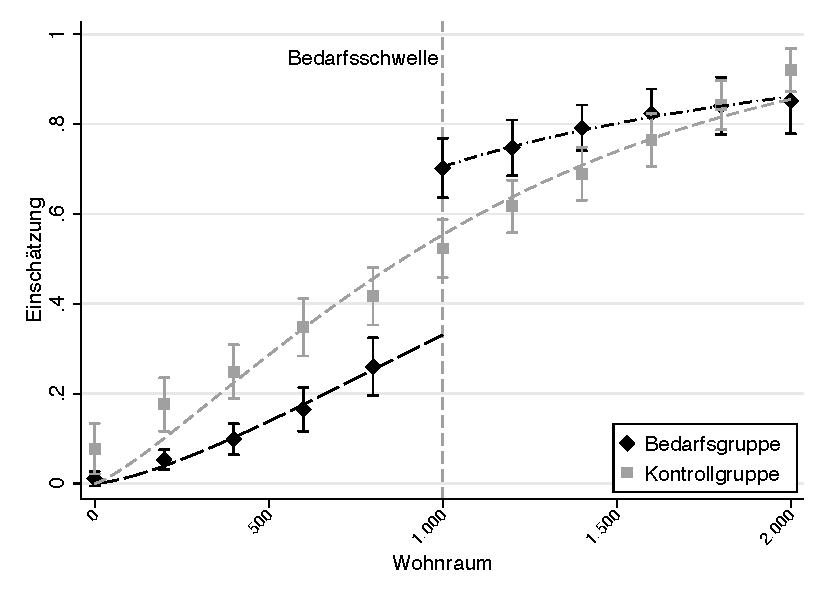
\includegraphics[width=0.99\linewidth]{figure_1.pdf}
   \caption{Durchschnittliche Gerechtigkeitseinschätzungen in der globalen Einschätzungsaufgabe nach Gruppe}
\end{figure}

Wir sind allerdings~-- wie eingangs bereits erwähnt~-- davon ausgegangen, dass die Gerechtigkeitsbewertungsfunktionen unserer Teilnehmer*innen (schwach) monoton steigend mit der Menge an zur Verfügung gestelltem Wohnraum sein sollten, dass wir auf dieser Skala also vorrangig positive Werte finden würden.
Außerdem haben wir angenommen, dass der marginale Anstieg der wahrgenommenen Gerechtigkeit mit zunehmender Menge an Wohnraum geringer ausfallen sollte, wir also bei der globalen Einschätzungsaufgabe in der Kontrollgruppe konkave Gerechtigkeitsbewertungsfunktionen beobachten würden (was im Folgenden als Monotoniehypothese bezeichnet wird).
In der Bedarfsgruppe wiederum sollte die Bedarfsschwelle als Referenzpunkt fungieren, von dem die Gerechtigkeitseinschätzungen entsprechend beeinflusst werden sollten.
Hier haben wir eine konvexe Gerechtigkeitsbewertungsfunktion unterhalb sowie eine konkave oberhalb der Schwelle erwartet, also eine Sigmoid- beziehungsweise, schöner gewendet, eine Schwanenhalsfunktion (was im Folgenden als Referenzpunkthypothese bezeichnet wird).
Dementsprechend haben wir auch bei der relativen Einschätzungsaufgabe nicht nur vermutet, dass die Gerechtigkeitsbewertungsfunktionen (schwach) monoton steigend sein sollten, sondern dass der Unterschied zwischen zwei Fällen umso höher ausfallen würde, je näher sie an einem Referenzpunkt (also bei 1.000 Einheiten in der Bedarfsgruppe beziehungsweise bei 0 Einheiten in der Kontrollgruppe) liegen.

\begin{figure}[t]\label{fig:abbildung_2}
   \center
   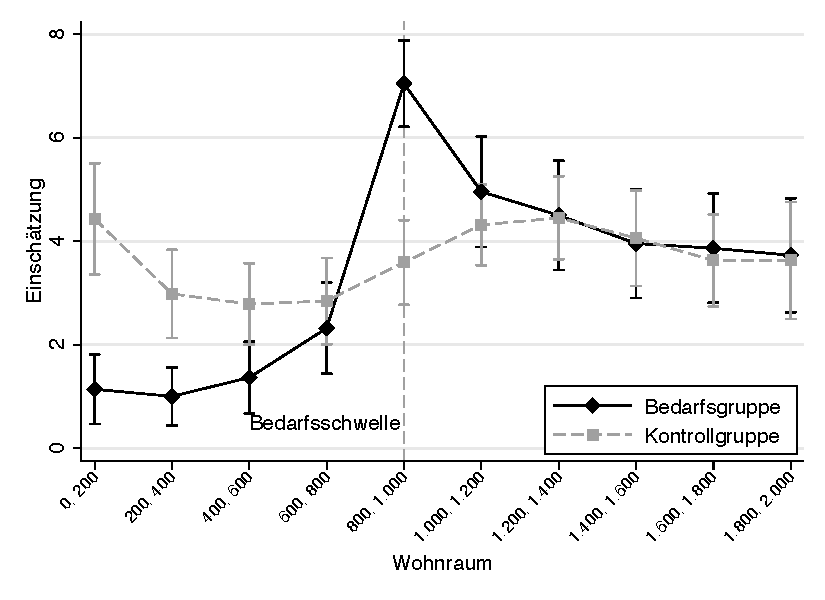
\includegraphics[width=0.99\linewidth]{figure_2.pdf}
   \caption{Durchschnittliche Gerechtigkeitseinschätzungen in der relativen Einschätzungsaufgabe nach Gruppe}
\end{figure}

Umgesetzt wurde die Studie mit \citet{limesurvey_limesurvey_2020}.
Die Teilnehmer*innen wurden rekrutiert über das \textit{Hamburg Registration and Organization Online Tool} \citep{bock_hroot_2014}.
Insgesamt haben 116 Personen im September 2016 im WiSo-Experimentallabor der Universität Hamburg an der Studie teilgenommen.
Ihr Medianalter betrug zum Zeitpunkt der Durchführung 25 Jahre; von denjenigen, die ihr Geschlecht angegeben haben (insgesamt 76\,\% der Teilnehmer*innen), waren 56\,\% weiblich, 42\,\% männlich und 2\,\% nichtbinär.
Die Teilnehmer*innen erhielten 10 Euro als Aufwandsentschädigung für ihre Teilnahme.
Die Sitzung dauerte insgesamt etwa eine Stunde und bestand aus zwei Studien zur Bedarfsgerechtigkeit, wobei die hier vorgestellte Studie an erster Stelle stattfand, also von der zweiten nicht beeinflusst werden konnte.

\begin{figure}[t]\label{fig:abbildung_3}
   \center
   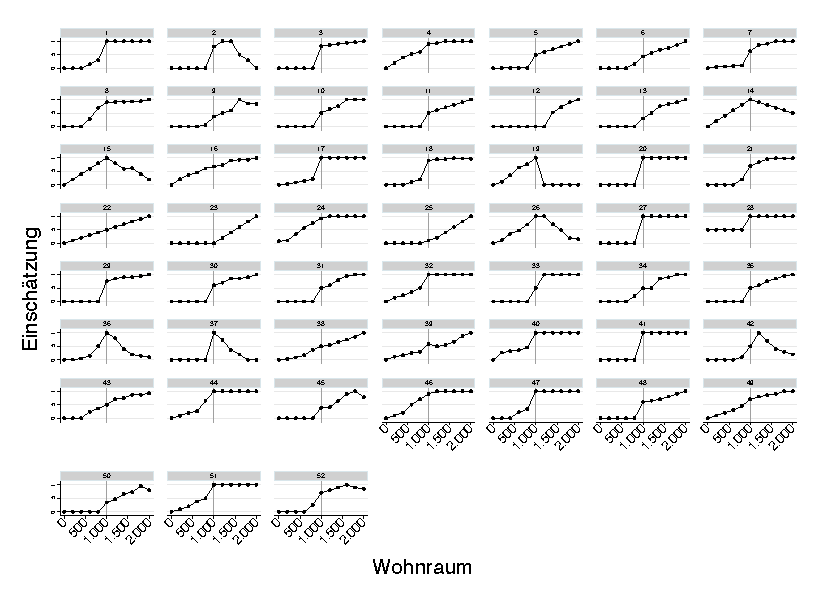
\includegraphics[width=0.99\linewidth]{figure_3.pdf}
   \caption{Individuelle Gerechtigkeitseinschätzungen in der globalen Einschätzungsaufgabe für die Bedarfsgruppe}
\end{figure}

Von den 57 Teilnehmer*innen in der Bedarfsgruppe sowie von den 59 Teilnehmer*innen in der Kontrollgruppe wurden von uns jeweils 5 beziehungsweise 2 Teilnehmer*innen von der Analyse ausgeschlossen, da sie ihre Schieberegler nicht bewegt hatten und wir demnach davon ausgegangen sind, dass sie keine Evaluation vorgenommen hatten.
Für die verbliebenen 52 Teilnehmer*innen in der Bedarfsgruppe sowie die verbliebenen 57 Teilnehmer*innen in der Kontrollgruppe zeigt Abbildung~\ref{fig:abbildung_1} die durchschnittlichen Gerechtigkeitseinschätzungen (normiert auf einen Bereich von 0 bis 1) sowie entsprechende 90-Prozent-Konfidenzintervalle in Abhängigkeit von der Menge an Wohnraum und getrennt nach Gruppe.
Es wird deutlich, dass die Einschätzungen in der Kontrollgruppe mit steigendem Wohnraum beinahe linear ansteigen.
In der Bedarfsgruppe gibt es jedoch einen sprunghaften Anstieg bei der Bedarfsschwelle.
Die durchschnittlichen Einschätzungen unterhalb der Bedarfsschwelle sind außerdem (ausgenommen die Situation mit 0 Einheiten) in der Bedarfsgruppe signifikant niedriger als in der Kontrollgruppe.
Auf und über der Bedarfsschwelle sind sie hier (ausgenommen die Situationen mit 1.600, 1.800 und 2.000 Einheiten) signifikant höher.
Die durchgän\-gige Linie stellt zusätzlich eine geschätzte Weibul-Verteilung für die Bedarfsgruppe (mit dem Referenzpunkt bei 1.000) und die gepunktete Linie für die Kontrollgruppe (mit dem Referenzpunkt bei 0) dar.
Die Schätzung für die Bedarfsgruppe ist unterhalb der Bedarfsschwelle konvex, weist einen Sprung von etwa 35 Prozentpunkten an der Bedarfsschwelle auf und setzt sich danach konkav fort.

Für die Auswertung der relativen Einschätzungsaufgabe haben wir dieselben 52 und 57 Teilnehmer*innen zugrunde gelegt.
Hier zeigt Abbildung~\ref{fig:abbildung_2}, dass die paarweisen Vergleiche in der Kontrollgruppe um 3 und 4 Punkte mäandern.
In der Bedarfsgruppe beobachten wir unterhalb der Schwelle jedoch relativ niedrige Werte, die (den Vergleich von 600 und 800 Einheiten ausgenommen) signifikant niedriger sind als in der Kontrollgruppe; hier wird der gerechtere Fall nur um 1 bis 2 Punkte besser eingeschätzt.
Mit Erreichen der Schwelle steigt der Wert auf 7 Punkte an, was signifikant höher als in der Kontrollgruppe ist.
Oberhalb der Schwelle resultieren die Vergleiche dann in Werten von etwa 3 bis 5 Punkten, ohne dass es hier einen nennenswerten Unterschied zwischen den Gruppen zu geben scheint.
Insgesamt untermauert dieses Bild die Ergebnisse der globalen Einschätzungsaufgabe und damit sowohl die Monotoniehypothese als auch die Referenzpunkthypothese.

\begin{figure}[t]\label{fig:abbildung_4}
   \center
   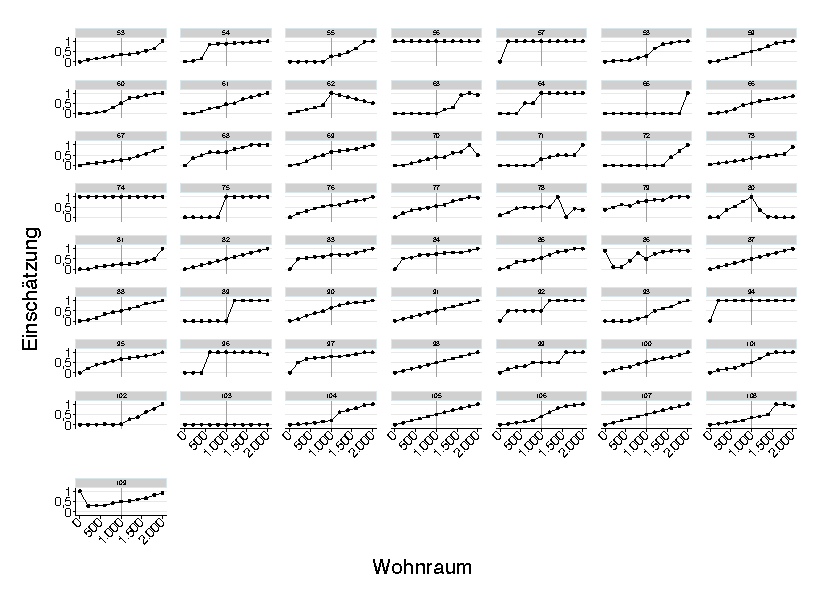
\includegraphics[width=0.99\linewidth]{figure_4.pdf}
   \caption{Individuelle Gerechtigkeitseinschätzungen in der globalen Einschätzungsaufgabe für die Kontrollgruppe}
\end{figure}

Abschließend werfen wir für die globale Einschätzungsaufgabe einen näheren Blick auf die Einschätzungen der einzelnen Teilnehmer*innen.
Abbildung~\ref{fig:abbildung_3} zeigt hier die Gerechtigkeitseinschätzungen der Teilnehmer*innen in der Bedarfs\-gruppe und Abbildung~\ref{fig:abbildung_4} der Teilnehmer*innen in der Kontrollgruppe als Liniendiagramme.
Obwohl es insgesamt relativ viel Heterogenität zu geben scheint, gehen wir davon aus, dass es im Detail verschiedene Muster gibt, die hier sichtbar werden.
In Tabelle~\ref{tab:typen} identifizieren wir dementsprechend vier verschiedene Typen.

In der Bedarfsgruppe gibt es, wie Abbildung~\ref{fig:abbildung_3} zeigt, 8 Teilnehmer*innen (15,38\,\%), deren Gerechtigkeitsbewertungsfunktion nicht (schwach) monoton steigend ist.
Ihre Bewertungen sind stattdessen eher hügelförmig; es gibt einen Anstieg bis zur oder knapp über die Bedarfsschwelle, ehe es wieder zu einem Abfall kommt, was anzeigt, dass es in ihren Augen ungerecht ist, wenn mehr Wohnraum als benötigt gebaut wird.
Das bezeichnen wir als eine \enquote{strikte} Form von Suffizientarismus.
4 Teilnehmer*innen (7,69\,\%) haben binäre Einschätzungen vorgenommen, die im Unterversorgungsbereich bei 0 oder nahe 0 und im Überversorgungsbereich bei 1 oder nahe 1 liegen.
Diese Art und Weise der Unterscheidung zwischen ungerechter Unterversorgung und Gerechter Versorgung nennen wir eine \enquote{qualitative} Form von Suffizientarismus.
Die Einschätzungen von 7 anderen Teilnehmer*innen (13,46\,\%) nehmen mit ansteigendem Wohnraum unterhalb der Bedarfsschwelle zu und erreichen mit der Bedarfsschwelle ein Maximum, das im Überversorgungsbereich anhält.
Diese graduelle Unterscheidung der Unterversorgung nennen wir eine \enquote{quantitative} Form von Suffizientarismus.
15 Teilnehmer*innen (28,85\,\%) haben die Unterversorgungsfälle als sehr ungerecht bewertet und steigende Einschätzungen im Überversorgungsbereich vorgenommen.
Hier sprechen wir von einer \enquote{strikten} Form von Prioritarismus.
Die Einschätzungen von weiteren 17 Teilnehmer*innen (32,69\,\%) steigen mit zunehmendem Wohnraum an, was wir als eine Form von Utilitarismus bezeichnen.

Ein Blick auf Abbildung~\ref{fig:abbildung_4} lässt vermuten, dass es in der Kontrollgruppe weniger Heterogenität gibt.
Hier haben wir es eine klare Mehrheit von insgesamt 36 Teilnehmer*innen (63,16\,\%), die sich als utilitaristisch klassifizieren lassen.
Daneben lassen sich aber interessanterweise auch Instanzen der anderen Typen finden.
In einigen Fällen spielt wieder der Fall mit 1.000 Einheiten Wohnraum eine besondere Rolle, obwohl es in der Kontrollgruppe keinerlei Hinweis auf eine Schwelle gegeben hat.
Das mag daran liegen, dass es sich bei 1.000 Einheit um die Hälfte der maximal möglichen 2.000 Einheiten handelt.

Diese Studie liefert uns Indikatoren dafür, dass das Vorliegen von Informationen über Bedürfnisse eine wichtige Rolle dabei spielen kann, wie Personen die Gerechtigkeit einer Verteilung einschätzen.
Offensichtlich spielt es eine Rolle für solche Einschätzungen, wie gut oder schlecht eine Partei hinsichtlich ihres Bedarfs versorgt ist.
Die Bedarfsschwelle, die angibt, ab welchem Punkt der Bedarf dieser Partei gedeckt ist, wirkt außerdem als ein Referenzpunkt, wobei Gerechtigkeitseinschätzungen dann~-- das lässt sich zumindest für unseren nichtkomparativen Zusammenhang sagen~-- relativ zu diesem Referenzpunkt stattfinden.

Ob eine solche Referenzpunktabhängigkeit aus normativer Perspektive wünschenswert ist oder nicht, steht dabei freilich auf einem anderen Blatt.
Das wird insbesondere in vergleichender Perspektive deutlich: Wenn eine Bedarfsschwelle von 1.000 Einheiten angenommen wird und es zwei Personen A und B gibt, wobei Person~A aktuell über 200 Einheiten verfügt und Person~B über 800 Einheiten, während es 200 weitere Einheiten gibt, die zur Verteilung stehen, dann ließe sich argumentieren, dass die schlechtergestellte Person diese zusätzlichen 200 Einheiten erhalten und somit von 200 auf insgesamt 400 Einheiten angehoben werden sollte.
Es ließe sich aber auch argumentieren, dass dem Erreichen der Bedarfsschwelle besondere Bedeutung zukommt, weswegen die 200 Einheiten stattdessen Person~B zugesprochen werden sollten, um sie von 800 auf insgesamt 1.000 Einheiten zu heben.


%%%%%%%%%%%%%%%%%
% VERANTWORTUNG %
%%%%%%%%%%%%%%%%%
\section{Bedarf und Verantwortung}\label{sec:verantwortung}
In unserer vorangegangenen Studie haben wir gesehen, dass Bedarfsinformationen einen Einfluss darauf hatten, wie unsere Teilnehmer*innen Verteilungssituationen als unparteiische Beobachter*innen einschätzten.
In dieser Studie haben wir die Rolle unserer Teilnehmer*innen hin zu unparteiischen Entscheider*innen verschoben.\footnote[][-0.7cm]{Diese Studie ist zuerst als Arbeitspapier erschienen \citep{bauer_need_2020} und später als \citet{bauer_need_2022} publiziert worden.}
Dazu haben wir ihnen eine Vignette präsentiert, in der sie gebeten wurden, sich zwei Personen vorzustellen.
Beide trugen einen anderen Namen, der für unsere Teilnehmer*innen zufällig aus einer Menge weit verbreiteter deutscher Nachnamen gezogen wurde.
Im Folgenden sprechen wir aber, der Einfachheit halber, von \enquote{Person~A} und \enquote{Person~B}.
Unseren Teilnehmer*innen wurde mitgeteilt, dass sich Person~A und Person~B nicht kennen würden.
Ihr Heim würden sie ausschließlich mit Feuerholz heizen, wobei jeder von ihnen ausreichend Feuerholz auf Lager habe, um den anstehenden Winter zu überleben.
Um sicherzugehen, dass sie nicht frieren müssen, würden sie allerdings zusätzliches Holz benötigen.
Die Gemeinde, in der beide leben, habe ihnen daher ermöglicht, für eine gewisse Zeit Holz im gemeindeeigenen Wald zu schlagen.
Da Person~A und Person~B über wenig Geld verfügen würden, wäre das ihre einzige Möglichkeit, zusätzliches Heizmaterial für den kommenden Winter zu erhalten.
Die Aufgabe unserer Teilnehmer*innen war es dann, die von beiden geschlagene Menge an Holz, ausgedrückt als Anzahl von Holzscheiten, möglichst gerecht zwischen Person~A und Person~B aufzuteilen.

\begin{table}[t]
   \caption{Typen von Einschätzungen}\label{tab:typen}
   \begin{center}
   \begin{tabular}{lrrrrrrl}
   \hline
   Typ              & \multicolumn{5}{c}{Häufigkeit}   &   & Prinzip                                                           \\
   \cline{2-6}
                    & \multicolumn{2}{c}{Bedarfsgr.}   &   & \multicolumn{2}{c}{Kontrollgr.}   &   &                           \\
   \hline\hline
   Hügelförmig      &  8   &  (15,38\,\%)              &   &  2   &   (3,51\,\%)               &   & \enquote{Strikter}        \\[-0.75ex]
                    &      &                           &   &      &                            &   & Suffizientarismus         \\[0.75ex]
   Binär            &  4   &   (7,69\,\%)              &   &  5   &   (8,77\,\%)               &   & \enquote{Qualitativer}    \\[-0.75ex]
                    &      &                           &   &      &                            &   & Suffizientarismus         \\[0.75ex]
   Flach ab         &  7   &  (13,46\,\%)              &   &  1   &   (1,75\,\%)               &   & \enquote{Quantitativer}   \\[-0.75ex]
   der Schwelle     &      &                           &   &      &                            &   & Suffizientarismus         \\[0.75ex]
   Null unterhalb   & 15   &  (28,85\,\%)              &   &  5   &   (8,77\,\%)               &   & \enquote{Strikter}        \\[-0.75ex]
   der Schwelle     &      &                           &   &      &                            &   & Prioritarismus            \\[0.75ex]
   Ansteigend       & 17   &  (32,69\,\%)              &   & 36   &  (63,16\,\%)               &   & Utilitarismus             \\[0.75ex]
   Anderes          &  1   &   (1,92\,\%)              &   &  8   &  (14,04\,\%)               &   &                           \\
   \hline
                    & 52   & (100,00\,\%)              &   & 57   & (100,00\,\%)               &   &                           \\
   \hline
   \end{tabular}
   \end{center}
\end{table}

Ohne jegliche Informationen wäre eine Gleichverteilung des Holzes hier vermutlich der~-- normative wie deskriptive~-- Modus der Wahl.
Unseren Teilnehmer*innen haben wir allerdings Informationen an die Hand gegeben, über die sich Ungleichverteilungen legitimieren ließen, indem wir Person~A und Person~B als heterogen hinsichtlich ihrer Produktivität sowie hinsichtlich ihres Bedarfs dargestellt haben.
Zwischen unseren Gruppen haben wir außerdem variiert, ob die bedürftigere respektive weniger produktive Person für ihren höheren Bedarf beziehungsweise für ihre niedrigere Produktivität selbst verantwortlich war oder nicht.

Die Variation von Bedarf und Produktivität fand innerhalb der Gruppen statt.
Hierzu wurden die Fälle, in denen unsere Teilnehmer*innen Verteilungsentscheidungen zu treffen hatten, in zwei Szenarien aufgeteilt, die unseren Teilnehmer*innen in zufälliger Reihenfolge vorgelegt wurden.
Im sogenannten \textit{Bedarfsszenario} waren beide Personen gleichermaßen produktiv; die Zahl der von ihnen geschlagenen Scheite unterschied sich nicht.
Dafür war die Ausprägung ihres Bedarfs sowohl von Person zu Person wie auch von Fall zu Fall unterschiedlich.
Im \textit{Produktivitätsszenario} dagegen unterschieden sie sich nicht in ihrem Bedarf, dafür aber in der Zahl der geschlagenen Scheite, die sich von Person zu Person und von Fall zu Fall unterschied.

Für die Variation der Verantwortlichkeit haben wir zwei Gruppen gebildet, denen unsere Teilnehmer*innen zu Beginn der Studie zufällig zugeteilt wurden.
In der sogenannten \textit{Verantwortlichkeitsgruppe} wurden sie darüber informiert, dass Person~A~-- die in jedem Fall die benachteiligte Person darstellte, also diejenige, deren Bedarf höher oder deren Produktivität niedriger war~-- weiterhin stark geraucht habe, obwohl ihr Arzt ihr davon abgeraten hätte.
Im Zuge dessen habe sie eine Stoffwechselkrankheit entwickelt, die wiederum der Grund dafür sei, dass sie (im Bedarfsszenario) eine höhere Raumtemperatur und daher mehr Holz benötigen würde oder dass sie (im Produktivitätsszenario) weniger Holz geschlagen habe.
In der \textit{Kontrollgruppe} hatte Person~A die gleichen Einschränkungen, allerdings sei ihre Krankheit hier angeboren gewesen, sie sei also nicht durch eigenes Zutun dafür verantwortlich.

\begin{table}[t]\label{tab:faelle}
   \caption{Parametrisierung der Studie nach Szenario und Fall}
   \begin{center}
   \begin{tabular}{lrrrrr}
   \hline
   Fall                   & \multicolumn{1}{c}{1} & \multicolumn{1}{c}{2} & \multicolumn{1}{c}{3} & \multicolumn{1}{c}{4} & \multicolumn{1}{c}{5} \\
   \hline\hline
                          & \multicolumn{5}{c}{Bedarfsszenario}                                                                                   \\
   \hline
   Bedarf A               & 1.800                 & 1.400                 & 1.000                 & 700                   & 600                   \\
   Bedarf B               & 1.200                 & 800                   & 400                   & 200                   & 100                   \\
   Produktivität A        & 1.000                 & 1.000                 & 1.000                 & 1.000                 & 1.000                 \\
   Produktivität B        & 1.000                 & 1.000                 & 1.000                 & 1.000                 & 1.000                 \\
   Gleichverteilung       & 1.000                 & 1.000                 & 1.000                 & 1.000                 & 1.000                 \\
   Anteil Bedarf A        & 0,60                  & 0,64                  & 0,71                  & 0,78                  & 0,86                  \\
   Anteil Produktivität A & 0,50                  & 0,50                  & 0,50                  & 0,50                  & 0,50                  \\
   \hline
                          & \multicolumn{5}{c}{Produktivitätsszenario}                                                                            \\
   \hline
   Bedarf A               & 1.000                 & 1.000                 & 1.000                 & 1.000                 & 1.000                 \\
   Bedarf B               & 1.000                 & 1.000                 & 1.000                 & 1.000                 & 1.000                 \\
   Produktivität A        & 1.200                 & 800                   & 400                   & 200                   & 100                   \\
   Produktivität B        & 1.800                 & 1.400                 & 1.000                 & 700                   & 600                   \\
   Gleichverteilung       & 1.500                 & 1.100                 & 700                   & 450                   & 350                   \\
   Anteil Bedarf A        & 0,50                  & 0,50                  & 0,50                  & 0,50                  & 0,50                  \\
   Anteil Produktivität A & 0,40                  & 0,36                  & 0,29                  & 0,22                  & 0,14                  \\
   \hline
   \end{tabular}
   \end{center}
\end{table}	

Unsere Teilnehmer*innen hatte pro Szenario Verteilungen für die fünf~-- insgesamt also zehn~-- verschiedenen Fälle vorzunehmen, die in Tabelle~\ref{tab:faelle} dargestellt sind.\footnote{Ein sechster Fall pro Szenario wurde von uns nur zur Prüfung der Konsistenz abgefragt und wird hier, nachdem sich keine Auffälligkeiten gezeigt haben, nicht weiter behandelt.}
Ihnen wurden dabei die absoluten Werte (also der Bedarf von Person~A und B sowie die Produktivität von Person~A und B) vorgelegt, die hier in Abbildung~\ref{fig:abbildung_5} zusätzlich~-- der besseren Lesbarkeit halber als Liniendiagramm~-- visualisiert werden (wobei im Bedarfsszenario die Produktivität von Person~A und Person~B sowie die Gleichverteilung und im Produktivitätsszenario der Bedarf von Person~A und Person~B bei jeweils 1.000 Holzscheiten zusammenfallen).

Mit diesem Aufbau wollten wir in erster Linie den Einfluss von Informationen über Bedarf, Produktivität und Verantwortlichkeit auf die Verteilungsentscheidungen unserer Teilnehmer*innen untersuchen.
Neu an unserem Aufbau war hier unter anderem die systematische Variation von Verantwortlichkeit für den höheren Bedarf einerseits sowie für die niedrigere Leistung andererseits.
Außerdem haben wir unsere Teilnehmer*innen das zur Verfügung stehende Holz frei verteilen lassen (mit der einzigen Restriktion, dass sie keine Scheite zurückhalten durften), anstatt~-- wie es bei vielen anderen Studien der Fall ist~-- ihnen eine Menge möglicher Verteilungen zur Auswahl vorzulegen.

\begin{figure}[t]\label{fig:abbildung_5}
   \center
   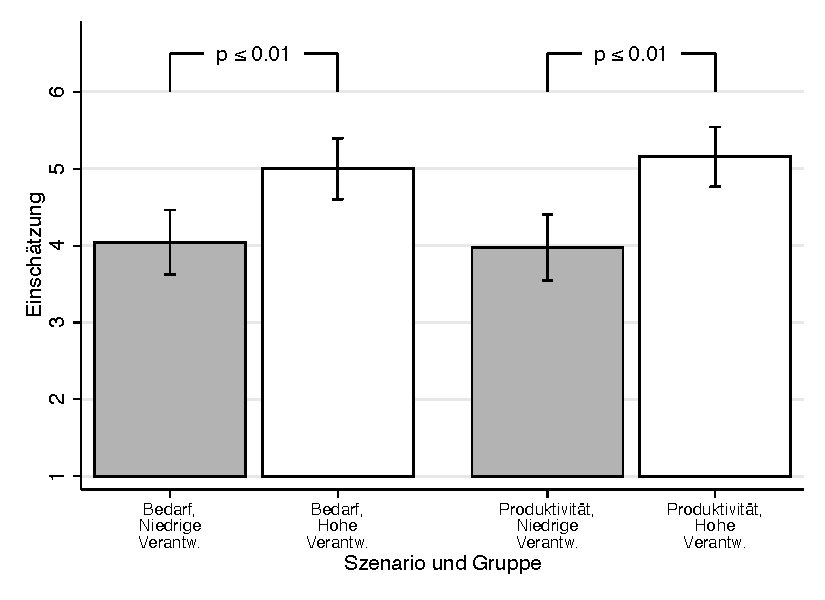
\includegraphics[width=0.99\linewidth]{figure_5.pdf}
   \caption{Parametrisierung der Studie nach Szenario und Fall}
\end{figure}

Im Lichte unserer ersten Studie sowie der bisher verfügbaren empirischen Literatur sind wir davon ausgegangen, dass die Teilnehmer*innen eine Vorstellung von Verteilungsgerechtigkeit haben und gewisse Verteilungen gerechter finden als andere.
Diese evaluative Dimension sollte sich auch in ihren Verteilungsentscheidungen widerspiegeln (umso mehr in Fällen, in denen sie~-- wie in unserer Studie~-- unbeteiligt sind und keinen eigenen Vorteil aus den Verteilungen ziehen können).
Wir sind also davon ausgegangen, dass die Verteilungsentscheidungen, die wir beobachten, die Verteilungsgerechtigkeitspräferenzen unserer Teilnehmer*innen offenlegen.
Dabei sollte sich uns zeigen, inwieweit Bedürfnisse eine Rolle spielen und welchen Einfluss die Faktoren, die wir variieren, auf diese Rolle haben.
Um das zu analysieren, haben wir zwei simple Maße konstruiert, die uns bei der Interpretation der Verteilungsentscheidungen helfen sollten.
Da die Anzahl der Holzscheite, die an Person~A und Person~B verteilt werden konnten, nicht über alle Fälle identisch war, haben wir zunächst und in der Hauptsache den normalisierten Anteil an Holzscheiten, die von unseren Teilnehmer*innen an Person~A, also die grundsätzlich schlechtergestellte Person, verteilt wurden, konstruiert.
Hierzu werden die in einem Fall an Person~A verteilten Holzscheite ($\gamma_{A}$) durch die insgesamt zur Verfügung stehenden Holzscheite ($\Gamma$), wie in (\ref{eq:holz}), dividiert.

\begin{equation}\label{eq:holz}
   \textrm{Anteil Holzscheite} = \frac{\gamma_{A}}{\Gamma}
\end{equation}

Ohne das Vorliegen weiterer Informationen kann man~-- wie oben schon erwähnt~-- von einer Gleichverteilung als Standardmodus ausgehen.
Ungleichverteilungen würden dementsprechend auf das Vorliegen von Faktoren hindeuten, denen Relevanz für die Verteilungsgerechtigkeit einer Situation zugesprochen wird.
Aus diesem Grund haben wir zusätzlich die normalisierte Abweichung von der Gleichverteilung zugunsten von Person~A konstruiert.
Zur Normalisierung haben wir hierzu zunächst den Bedarfs- und Produktivitätsanteil von Person~A bestimmt, der sich, wie in (\ref{eq:bedarf}) und (\ref{eq:produktivitaet}) dargestellt, durch eine Division des Bedarfs von Person~A ($\nu_{a}$) und des Gesamtbedarfs ($N$) beziehungsweise der Produktivität von Person~A ($\phi_{A}$) und der Gesamtproduktivität ($\Phi$) ergibt.

\begin{equation}\label{eq:bedarf}
   \textrm{Anteil Bedarf} = \frac{\nu_{A}}{N}
\end{equation}

\begin{equation}\label{eq:produktivitaet}
   \textrm{Anteil Produktivität} = \frac{\phi_{A}}{\Phi}
\end{equation}

In unserer Parametrisierung bewegt sich der Bedarfsanteil von Person~A zwischen 60\,\% (in Fall 1) und 86\,\% (in Fall 5), der Produktivitätsanteil zwischen 14\,\% (in Fall 5) und 40\,\% (in Fall 1).
Hieraus haben wir dann die Abweichung wie in (\ref{eq:abweichung}) entweder als Verhältnis von Anteil Holzscheite abzüglich 0,5 und Anteil Bedarf abzüglich 0,5 (für das Bedarfsszenario) oder als Verhältnis von 0,5 abzüglich Anteil Holzscheite und 0,5 abzüglich Anteil Produktivität (für das Produktivitätsszenario) berechnen können.

\begin{equation}\label{eq:abweichung}
   \textrm{Abweichung} = \left\{\begin{array}{ll}\frac{\textrm{Anteil Holzscheite}-0,5}{\textrm{Anteil Bedarf}} & \textrm{(Bedarfsszenario)}\\ \\
   \frac{0,5-\textrm{Anteil Holzscheite}}{0,5-\textrm{Anteil Produktivität}} & \textrm{(Produktivitätsszenario)}
   \end{array}
   \right.
\end{equation}

Hierdurch erhalten wir im Bedarfsszenario einen Wert von 0, wenn Person~A lediglich das zugesprochen bekommt, was sie produziert hat, und 1, wenn ihr das zugesprochen wird, was sie benötigt.
Analog erhalten wir im Produktivitätsszenario einen Wert von 0, wenn Person~A erhält, was sie benötigt, und einen Wert von 1, wenn sie erhält, was sie produziert hat.
Dabei sind freilich auch Fälle denkbar, die außerhalb dieses Intervalls liegen.
Wenn Person~A im Bedarfsszenario beispielsweise mehr erhält, als sie benötigt, steigt der Wert über 1; erhält sie weniger, als sie produziert hat, sinkt er unter 0.
Im Produktivitätsszenario steigt der Wert analog über 1, wenn Person~A weniger bekommt, als sie produziert hat, und er fällt unter 0, wenn sie mehr erhält, als sie benötigt.
Wir sind allerdings davon ausgegangen, dass es im Rahmen unserer Vignette für solche Verteilungen kaum normative Gründe geben sollte.
Im Bedarfsszenario beispielsweise haben beide Personen durchgehend 1.000 Holzscheite geschlagen, es stehen also insgesamt 2.000 Scheite zur Verfügung.
Hier gibt es~-- wie sich in Tabelle~\ref{tab:faelle} zeigt~-- nur zwei Fälle, in denen Person~A mehr Holz geschlagen hat, als sie benötigt (nämlich in den Fällen 4 und 5).
In diesen Fällen lässt sich freilich davon ausgehen, dass Person~A auch mehr Holz zugesprochen bekommen würde, als sie benötigt, weil sich hier ohne größere Bedenken dem Leistungsprinzip folgen ließe.
In den verbleibenden Fällen des Bedarfsszenarios jedoch hat Person~A entweder genauso viel geschlagen, wie sie benötigt (nämlich in Fall 3), oder sie hat weniger geschlagen, als sie benötigt (nämlich in den Fällen 1 und 2).
Hier gilt es nun, zwischen dem Leistungs- und dem Bedarfsprinzip abzuwägen.
Da Person~B weder einen höheren Bedarf noch eine höhere Produktivität als Person~A hat, wird unseren Versuchsteilnehmer*innen kein Anreiz geboten, Person~A in diesem Szenario weniger zu geben, als sie produziert hat.
Wenn Person~A so viel erhält, wie sie geschlagen hat, muss aber auch ihr Bedarf unerfüllt bleiben.
Soll dem höheren Bedarf von Person~A Rechnung getragen werden, muss ihr mehr gegeben werden, als sie selbst geschlagen hat, was gleichzeitig dazu führt, dass Person~B weniger erhält, als sie geschlagen hat.
Die Beachtung des Bedarfs von Person~A geht also zu einem gewissen Grad mit einer Missachtung der Leistung von Person~B einher.
Das Leistungsprinzip stellt hier dementsprechend ein Gegengewicht zum Bedarfsprinzip dar, weswegen Person~A~-- in Fällen, in denen sie mehr benötigt als sie geschlagen hat~-- vielleicht mehr zugesprochen wird, als sie selbst produziert hat, sie aber nicht über ihre Bedarfsschwelle hinaus versorgt wird, weil dies noch weiter zu Lasten von Person~B gehen würde, ohne weiterhin durch das Bedarfsprinzip begründbar zu sein.
Tatsächlich lässt sich davon ausgehen, dass unsere Versuchsteilnehmer*innen sowohl den Bedarf als auch die Leistung von beiden Personen berücksichtigen, weswegen unsere Beobachtungen sich größtenteils innerhalb des Wertebereichs von 0 bis 1 bewegen sollten.

Insgesamt gab es vier Hypothesen, die wir mit unseren Daten und unter Zuhilfenahme der beiden Maße überprüfen wollten.
Zunächst einmal haben wir erwartet, dass Person~A, die immer schlechtergestellt ist als Person~B, weil sie entweder mehr benötigt oder weniger geleistet hat, von unseren Teilnehmer*innen zumindest teilweise für ihren jeweiligen Nachteil kompensiert wird, dass sie also im Durchschnitt mehr zugeteilt bekommt, als sie produziert hat, aber weniger, als sie benötigt (hier sprechen wir im Folgenden von der Kompensationshypothese).
Im Bedarfsszenario haben Person~A und Person~B jeweils gleich viel Holz geschlagen.
Person~A benötigt jedoch mehr davon als Person~B und in einem Teil der Fälle außerdem mehr, als sie selbst geschlagen hat.
Im Großen und Ganzen sind wir hier davon ausgegangen, dass Person~A nicht weniger zugesprochen werden sollte, als sie selbst geschlagen hat, dass 0,5 hier also die theoretische Untergrenze des von uns beobachteten Anteils darstellen sollte.
Im Produktivitätsszenario wiederum haben Person~A und Person~B einen gleich hohen Bedarf an Holz, wobei Person~A weniger als Person~B geschlagen hat und in einem Teil der Fälle außerdem weniger, als sie benötigt.
Hier sind wir davon ausgegangen, dass Person~A nicht mehr zugesprochen werden sollte, als sie benötigt, dass 0,5 in diesem Szenario also die theoretische Obergrenze darstellen sollte.
Wir haben dementsprechend erwartet, dass der Anteil, der Person~A von unseren Teilnehmer*innen zugesprochen wird, im Bedarfsszenario (wo er höher als 0,5 ausfallen sollte) größer sein sollte als im Produktivitätsszenario (wo er geringer als 0,5 ausfallen sollte).
Die Abweichung von der Gleichverteilung sollte bei diesen Grenzen~-- wie oben dargestellt~-- zwischen 0 und 1 liegen.

Die Bereitschaft, Person~A für ihren Nachteil zu kompensieren, sollte außerdem sinken, wenn sie selbst dafür verantwortlich ist, mehr Holz zu benötigen beziehungsweise weniger Holz geschlagen zu haben (was wir die Verantwortlichkeitshypothese nennen).
Der Anteil an Holz, der Person~A zugesprochen wird, sollte in der Verantwortlichkeitsgruppe entsprechend niedriger ausfallen als in der Kontrollgruppe.
Im Bedarfsszenario haben wir außerdem eine geringere Abweichung von der Gleichverteilung erwartet, sind also davon ausgegangen, dass unsere Teilnehmer*innen sich in der Verantwortlichkeitsgruppe mehr an der gleichen Produktivität als an den ungleichen Bedürfnissen orientieren würden.
Im Produktivitätsszenario wiederum haben wir eine größere Abweichung von der Gleichverteilung in der Verantwortlichkeitsgruppe erwartet, weil wir davon ausgegangen sind, dass Person~A weniger für ihre geringere Produktivität kompensiert werden sollte, womit sich die Zahl der zugesprochenen Scheite also von der Gleichverteilung hin zu der niedrigeren eigenen Produktivität verschieben würde (siehe auch Abbildung~\ref{fig:abbildung_5}).

Bedarfs- und Produktivitätsszenario sind außerdem spiegelbildlich angelegt: Wo Person~A beispielsweise einen Bedarfsanteil von 0,6 im Bedarfsszenario aufweist, hat sie einen Produktivitätsanteil von 0,4 im Produktivitätsszenario; wo ihr Bedarfsanteil 0,64 beträgt, ist ihr Produktivitätsanteil entsprechend 0,36 und so weiter.
Wir sind an dieser Stelle davon ausgegangen, dass der Anteil, der Person~A zugesprochen wird, sich nicht an den absoluten Kennzahlen, sondern an diesen relativen Zahlen, also am Bedarfs- und Produktivitätsanteil von Person~A, orientieren sollte.
Dementsprechend haben wir erwartet, dass die Anteile, die wir in beiden Szenarien beobachten, äquivalent zueinander sein sollten (hier sprechen wir im Folgenden von der Symmetriehypothese).
Der Anteil im Bedarfsszenario sollte dann 1 abzüglich des Anteils im Produktivitätsszenario entsprechen (da beispielsweise einem Bedarfsanteil von 0,6 ein Produktivitätsanteil von 0,4 gegenübersteht, womit gilt 1 – 0,4 = 0,6).
Die Abweichung von der Gleichverteilung sollte sich dementsprechend nicht zwischen den Szenarien unterscheiden.

Abschließend haben wir einen Blick auf die einzelnen Fälle geworfen. Diese sind im Bedarfsszenario so angelegt, dass der relative Anteil von Person~A am Gesamtbedarf von Fall 1 (mit 60\,\%) zu Fall 5 (mit 86\,\%) ansteigt.
In diesem Sinne nimmt die Ungleichheit hinsichtlich des Bedarfs von Person~A und Person~B von Fall 1 zu Fall 5 kontinuierlich zu.
Im Produktivitätsszenario sinkt der relative Anteil von Person~A an der Gesamtproduktivität von Fall 1 (mit 40\,\%) zu Fall 5 (mit 14\,\%) ab.
Hier nimmt also wiederum die Ungleichheit hinsichtlich der Produktivität von Person~A und Person~B von Fall 1 zu Fall 5 kontinuierlich zu (siehe auch Tabelle~\ref{tab:faelle}).
Wir haben vermutet, dass diese Veränderungen einen Einfluss auf den Anteil haben sollten, den unsere Teilnehmer*innen Person~A zusprechen (was wir im Folgenden als Anteiligkeitshypothese bezeichnen).
Im Bedarfsszenario sind wir davon ausgegangen, dass die Teilnehmer*innen Person~A mehr Holz zuteilen würden, wenn in einem Fall größere Ungleichheit hinsichtlich des Bedarfs von Person~A und Person~B herrscht.
Im Produktivitätsszenario wiederum haben wir vermutet, dass sie Person~A weniger Holz zuteilen würden, wenn eine größere Ungleichheit hinsichtlich der Produktivität von Person~A und Person~B vorliegt.
Die Abweichung von der Gleichverteilung sollte auch hier, da sie in dieser Hinsicht normalisiert ist, nicht betroffen sein.
Dieser Effekt könnte dadurch abgeschwächt werden, dass diejenigen Fälle mit größerer Ungleichheit im Bedarfsszenario die Versorgungssituation von Person~A verbessern und gleichzeitig diejenigen im Produktivitätsszenario ihre Versorgungssituation verschlechtern.

Programmiert wurde diese Studie mit \textit{oTree} \citep{chen_otree_2016}.
Für die Durchführung im September 2019 wurden unsere Teilnehmer*innen zufällig aus dem Online-Access-Panel des Marktforschungsunternehmens \textit{respondi} gezogen, wobei die Zusammensetzung stratifiziert war nach den Charakteristika Geschlecht (weiblich: 49,5\,\%, männlich: 50,5\,\%), Alter (18--29 Jahre: 20,5\,\%, 30--39 Jahre: 18,5\,\%, 40--49 Jahre: 19,0\,\%, 50--59 Jahre: 24,0\,\%, 60--69 Jahre: 18,0\,\%) sowie Nettoäquivalenzhaushaltseinkommen (0--1.099 Euro: 20,0\,\%, 1.100--1.499 Euro: 20,0\,\%, 1.500--1.999 Euro: 20,0\,\%, 2.000--2.599 Euro: 20,0\,\%, 2.600 und mehr Euro: 20,0\,\%).
Der internen Validität halber haben unsere Teilnehmer*innen nach dem Hauptteil der Studie insgesamt drei Kontrollfragen vorgelegt bekommen.
Wer mehr als eine dieser Fragen falsch beantwortet hat, ist aus der Studie ausgeschlossen worden.
Insgesamt 200 Teilnehmer*innen haben erfolgreich an der Studie teilgenommen und wurden für etwa 30 Minuten Bearbeitungszeit mit 4,90 Euro kompensiert.

\begin{figure}[t]\label{fig:abbildung_6}
   \center
   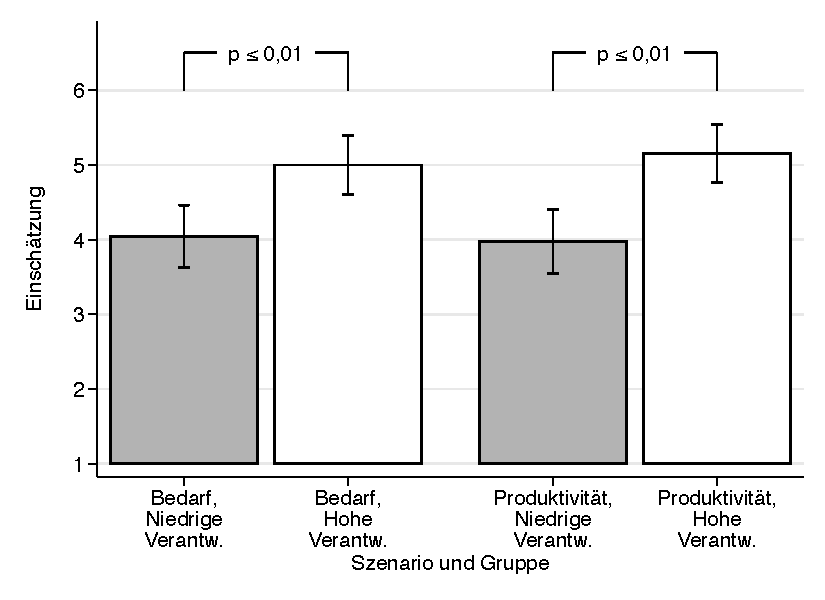
\includegraphics[width=0.99\linewidth]{figure_6.pdf}
   \caption{Durchschnittliche Einschätzung der Verantwortlichkeit nach Szenario und Gruppe}
\end{figure}

Nach dem Hauptteil der Studie sowie den Kontrollfragen mussten unsere Teilnehmer*innen eine Reihe von Anschlussfragen beantworten.
Hier wurden sie unter anderem gefragt, wie sehr sie Person~A als verantwortlich für ihre im Vergleich zu Person~B nachteilige Situation halten würden.
Abbildung~\ref{fig:abbildung_6} zeigt die durchschnittlichen Einschätzungen in der Verantwortlichkeits- sowie der Kontrollgruppe auf einer Skala von 1 (\enquote{überhaupt nicht verantwortlich}) bis 7 (\enquote{vollkommen verantwortlich}).
Wie erwartet~-- und durch einen zweiseitigen doppelten \textit{t}-Test bestätigt~-- wird die Verantwortung von Person~A in der Verantwortlichkeitsgruppe signifikant höher eingeschätzt als in der Kontrollgruppe.
Wir haben die Verantwortlichkeitsvariation zwischen unseren Gruppen also erfolgreich implementiert, wobei es~-- wie ein gepaarter zweiseitiger \textit{t}-Test zeigt~-- keinen Unterschied macht, ob Person~A nun für ihren höheren Bedarf oder ihre niedrigere Leistung verantwortlich ist.

Mit dieser Gewissheit im Hinterkopf haben wir uns als nächstes der eigentlichen Aufgabe unserer Teilnehmer*innen zuwenden können, bei der sie eigene Verteilungsentscheidungen zu treffen hatten.
Hier haben wir zunächst einen Blick auf die durchschnittlichen Verteilungen geworfen.
Bei der Analyse des Anteils und der Abweichung haben wir hier und im Folgenden alle 2.000 Verteilungsentscheidungen berücksichtigt, also alle 10 Entscheidungen von allen 200 Teilnehmer*innen.
Wie erwartet sind bei der Abweichung tatsächlich nur 208 Beobachtungen (also 10,4\,\%) kleiner als 0 oder größer als 1.

\begin{figure}[t]\label{fig:abbildung_7}
   \centering
   \caption{Anteil (linke Paneele) und Abweichung (rechte Paneele) nach Szenario und Gruppe (obere Paneele), nach Fall im Bedarfsszenario (mittlere Paneele) sowie nach Fall im Produktivitätsszenario (untere Paneele)}
   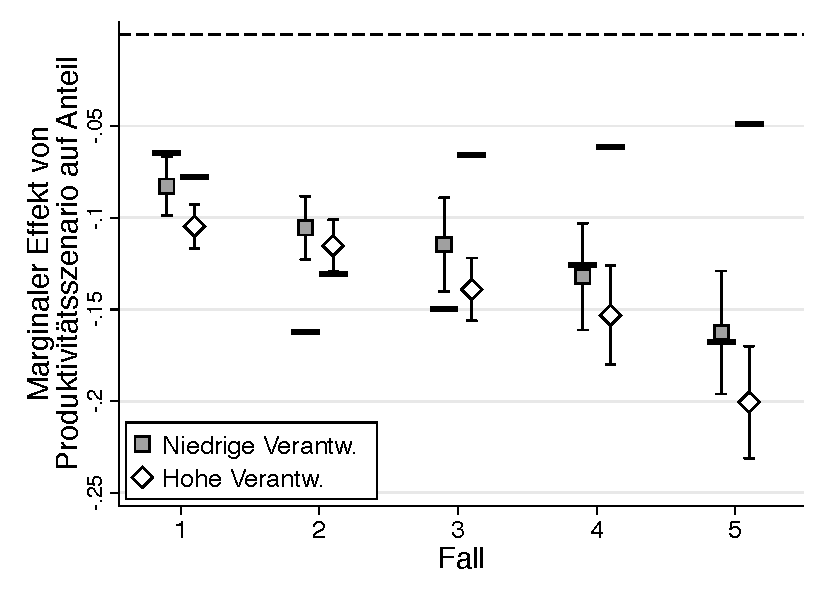
\includegraphics[width=0.49\linewidth]{figure_7_a.pdf}
   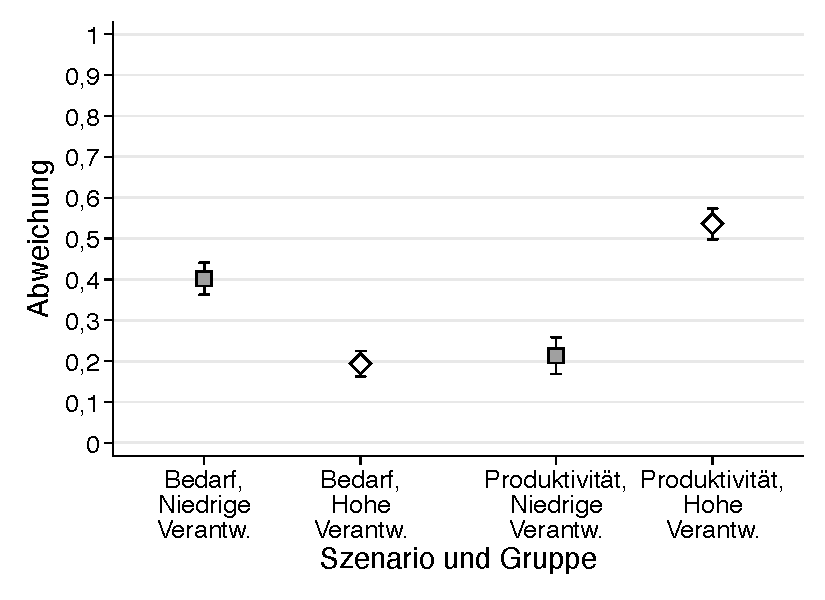
\includegraphics[width=0.49\linewidth]{figure_7_b.pdf}
   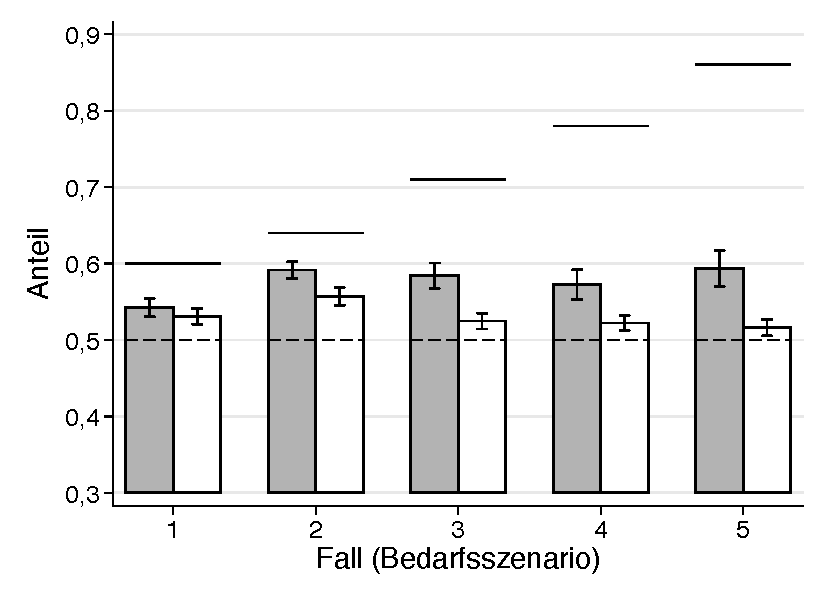
\includegraphics[width=0.49\linewidth]{figure_7_c.pdf}
   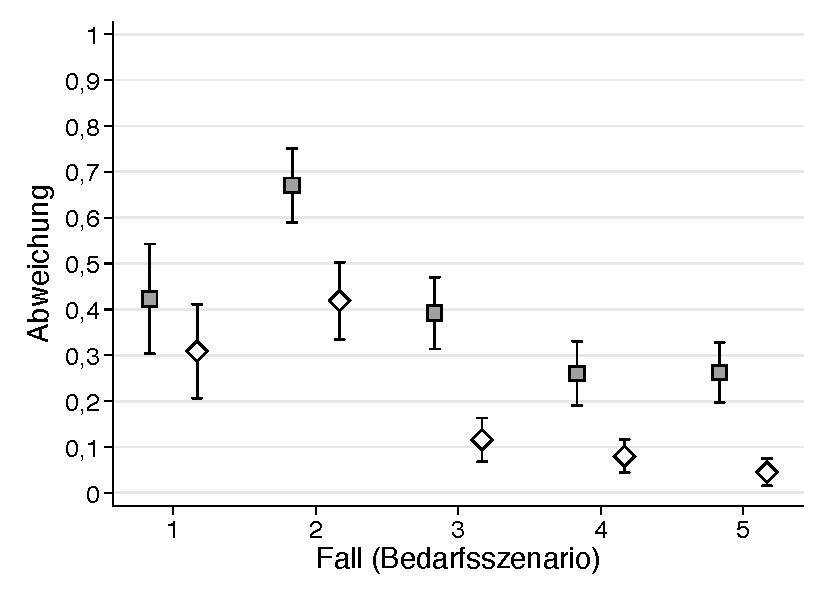
\includegraphics[width=0.49\linewidth]{figure_7_d.pdf}
   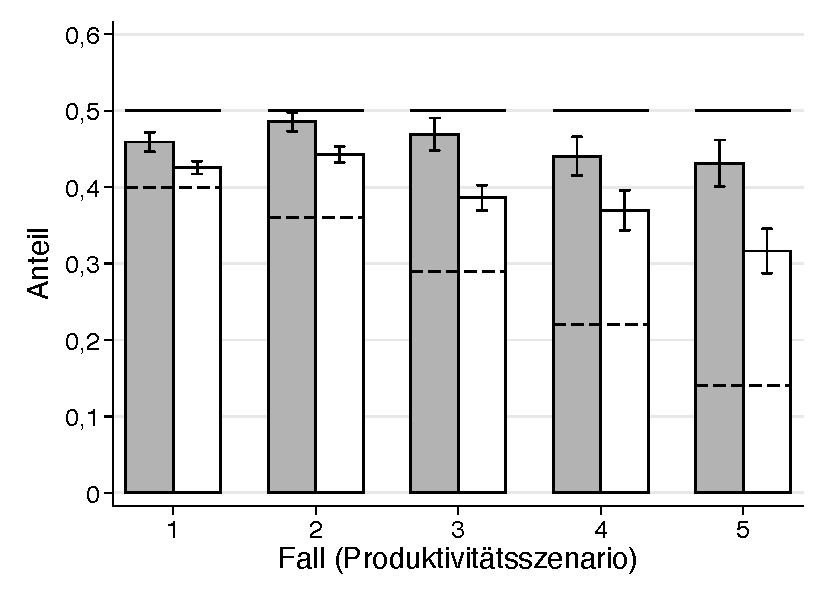
\includegraphics[width=0.49\linewidth]{figure_7_e.pdf}
   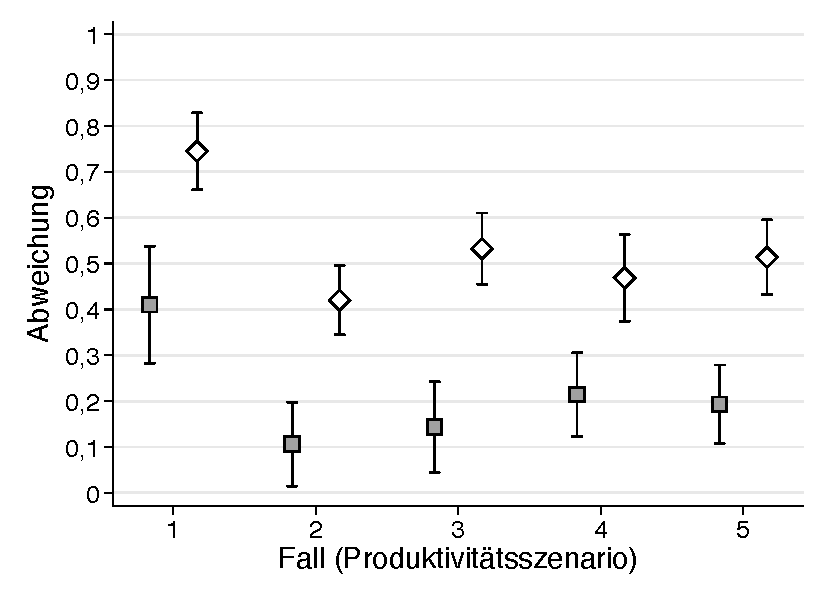
\includegraphics[width=0.49\linewidth]{figure_7_f.pdf}
\end{figure}

Abbildung~\ref{fig:abbildung_7} stellt im linken Paneel den durchschnittlichen Anteil sowie im rechten Paneel die durchschnittliche Abweichung (jeweils mit 90-Prozent-Konfidenz\-intervallen) dar.
Auf der linken Seite stellen die zusätzlich dargestellten durchgehenden Linien den Bedarfsanteil und die gestrichelten den Produktivitätsanteil von Person~A dar.
Es zeigt sich, dass der durchschnittliche Anteil durchweg zwischen diesen Linien liegt und~-- wie einseitige \textit{t}-Tests zeigen~-- in allen Gruppen (im oberen Paneel) sowie Szenarien und Fällen (im mittleren Paneel mit den Fällen des Bedarfs- und im unteren Paneel mit jenen des Produktivitätsszenarios) signifikant höher ausfällt als der Produktivitätsanteil und niedriger als der Bedarfsanteil, was unsere Kompensationshypothese stützt.
Auch unsere Verantwortlichkeitshypothese findet Stützung; der Effekt zwischen den Gruppen ist deutlich sichtbar und erweist sich~-- durch einseitige \textit{t}-Tests~-- in allen Fällen (außer dem ersten des Bedarfsszenarios) als signifikant.
Bei der Abweichung, die auf der rechten Seite dargestellt wird, erweisen sich ebenfalls alle Fälle als signifikant, wobei die Effekte im Bedarfsszenario entsprechend negativ und im Produktivitätsszenario positiv ausfallen.

\begin{figure}[t]\label{fig:abbildung_8}
   \centering
   \caption{Marginale Effekte von Produktivitätsszenario (obere Paneele) und Verantwortlichkeitsgruppe (untere Paneele) auf Anteil (linke Paneele) und Abweichung (rechte Paneele)}
   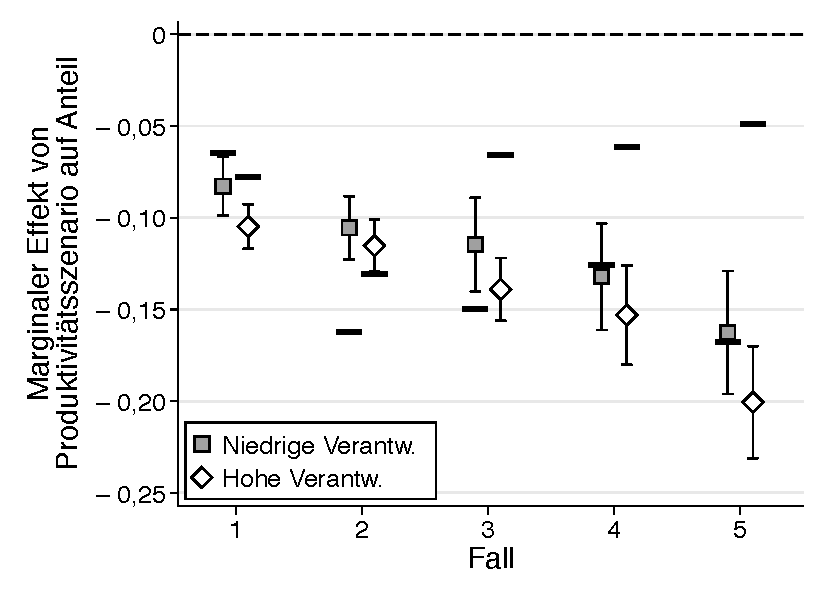
\includegraphics[width=0.49\linewidth]{figure_8_a.pdf}
   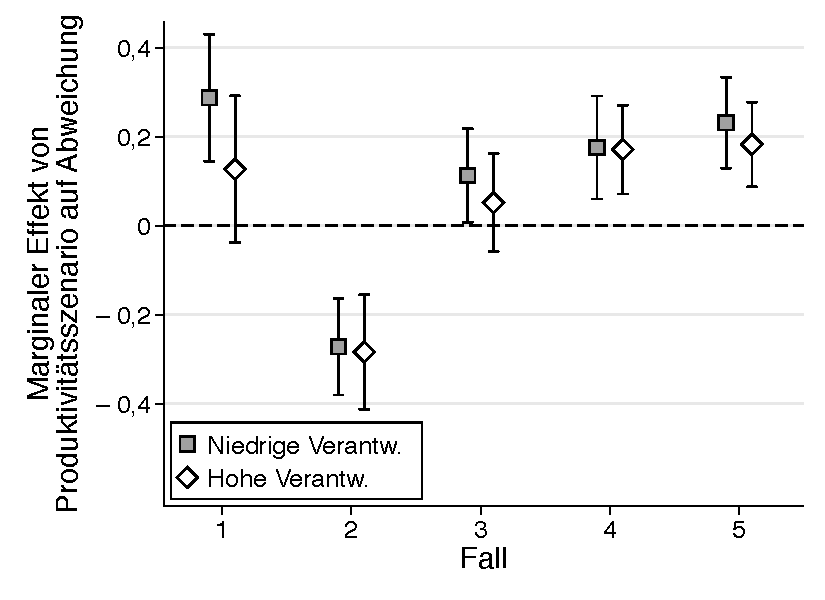
\includegraphics[width=0.49\linewidth]{figure_8_b.pdf}
   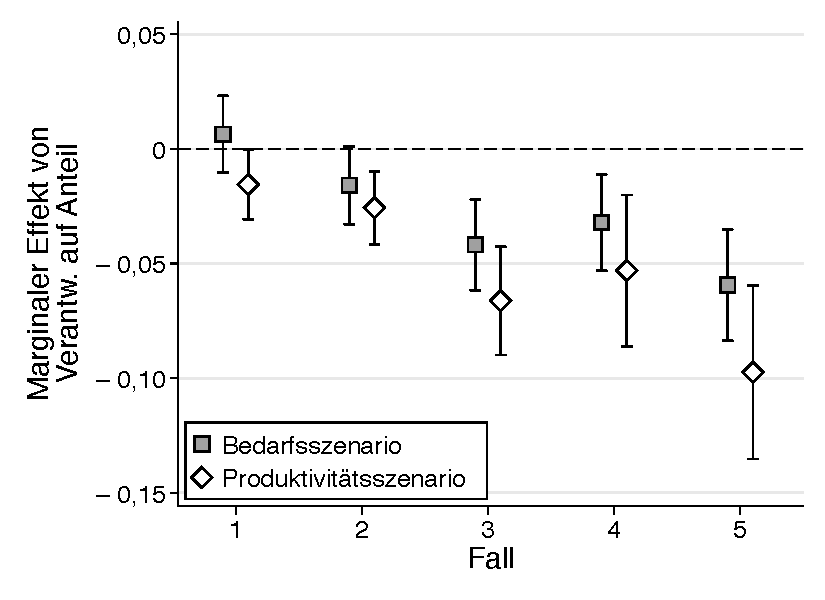
\includegraphics[width=0.49\linewidth]{figure_8_c.pdf}
   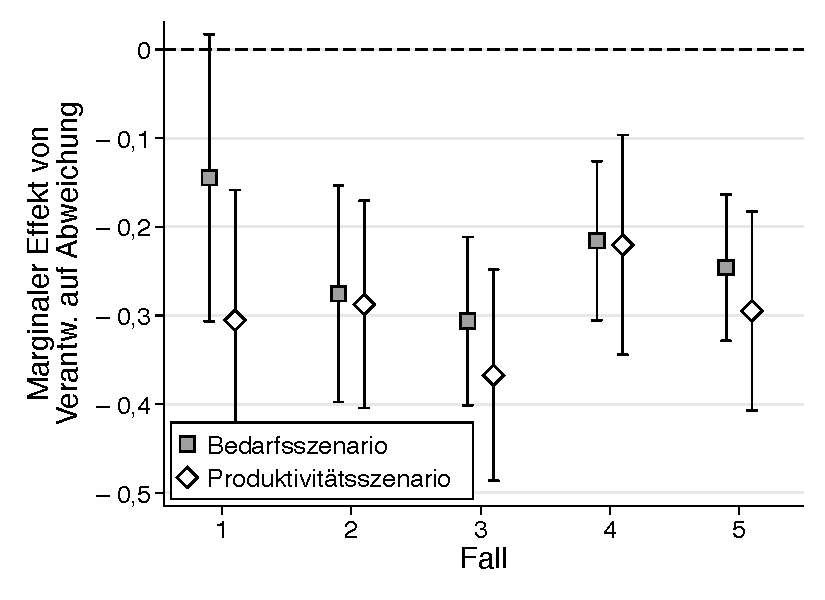
\includegraphics[width=0.49\linewidth]{figure_8_d.pdf}
\end{figure}

Um unter anderem auf den soziodemographischen Hintergrund unserer Teilnehmer*innen sowie auf mögliche Reihenfolgeneffekte kontrollieren zu können, haben wir ferner GLS-Panelregressionen mit zufälligen Effekten und robusten Standardfehlern durchgeführt, bei denen entweder der Anteil oder die Abweichung als endogene Variable fungierten.
Auf Grundlage dieser Regressionen haben wir außerdem die verbleibenden beiden Hypothesen in den Blick genommen.
Die marginalen Effekte von Szenario und Gruppe, die durch unsere \enquote{vollständigen} Modelle geschätzt werden, sind (für den Anteil in den linken sowie für die Abweichung in den rechten Paneelen) graphisch dargestellt in Abbildung~\ref{fig:abbildung_8}.

Das obere linke Paneel zeigt den marginalen Effekt des Produktivitätsszenarios auf den Anteil, den Person~A zugesprochen bekommt, für jeden der fünf Fälle in beiden Gruppen.
Hier erweisen sich alle marginalen Effekte (mit Ausnahme des ersten) als negativ signifikant, was unsere Kompensationshypothese weiter stützt.
Die marginalen Effekte des Szenarios unterscheiden sich (außer für Fall 1) nicht nennenswert zwischen den Gruppen.
In diesem Paneel sind außerdem, durch die schwarzen Linien, die Referenzwerte dargestellt, anhand derer wir unsere Symmetriehypothese getestet haben, bei der wir davon ausgegangen sind, dass der Anteil von Person~A im Produktivitätsszenario symmetrisch ist zu ihrem Anteil im Bedarfs\-szenario.
Der geschätzte marginale Effekt des Produktivitätsszenarios ist gleich dem Anteil von Person~A im Produktivitätsszenario abzüglich des Anteils von Person~A im Bedarfs\-szenario.
Wenn Symmetrie herrscht, sollte dieser marginale Effekt hier also 1 abzüglich des doppelten Anteils im Bedarfsszenario entsprechen.
Es zeigt sich, dass wir die Symmetriehypothese in der Kontrollgruppe zumindest für die Fälle 2 und 3 zurückweisen müssen; in der Verantwortlichkeitsgruppe sogar für alle Fälle außer Fall 2.
Bei paarweisen Vergleichen der marginalen Effekte des Produktivitätsszenarios sehen wir außerdem, dass dessen negativer Einfluss in den Fällen 4 und 5 signifikant höher ist als in Fall 1, was für unsere Anteiligkeitshypothese spricht, der zufolge höhere Ungleichheit zwischen Person~A und Person~B hinsichtlich ihres Bedarfs respektive ihrer Produktivität auch zu einem höheren Unterschied zwischen den Szenarien hinsichtlich des Anteils, den Person~A erhält, führen sollte.

Im oberen rechten Paneel sind die marginalen Effekte des Produktivitätsszenarios auf die Abweichung für jeden der fünf Falle visualisiert.
Sämtliche marginalen Effekte sind (mit Ausnahme von Fall 2 in beiden Gruppen sowie von Fall 1 und Fall 3 in der Verantwortlichkeitsgruppe) positiv signifikant, weichen also mit einem positiven Wert nennenswert von der dargestellten Nulllinie ab.
Würden die beiden Szenarien symmetrisch behandelt werden, sollten keine solchen Abweichungen feststellbar sein, weswegen auch dieses Ergebnis gegen unsere Symmetriehypothese spricht.
Offensichtlich ist die Abweichung von der Gleichverteilung, wie sich schon bei der Analyse des Anteils abgezeichnet hat, größer, wenn der Nachteil von Person~A durch geringere Produktivität statt durch höheren Bedarf entsteht.

Im unteren linken Paneel sehen wir den marginalen Effekt der Verantwortlichkeitsgruppe auf den Anteil nach Szenario und Fall.
Hier sind (mit Ausnahme von Fall 1 und 2 im Bedarfsszenario) alle marginalen Effekte negativ signifikant, was unsere Verantwortlichkeitshypothese weiter stützt.
Die Verantwortlichkeit hat einen klaren negativen Effekt auf den Anteil, der Person~A zugesprochen wird.
Dieser negative Effekt ist in den Fällen 4 und 5 außerdem signifikant stärker ausgeprägt als in Fall 1, was weiter für unsere Anteiligkeitshypothese spricht.

Im unteren rechten Paneel schließlich wird der marginale Effekt der Verantwortlichkeitsgruppe auf die Abweichung nach Szenario und Fall dargestellt.
Da wir im Bedarfsszenario einen marginalen Effekt größer 0 und im Produktivitätsszenario kleiner 0 erwartet haben, stellen wir hier der Einfachheit halber den negativen absoluten marginalen Effekt dar.
Es zeigt sich, dass dieser~-- in allen Fällen signifikante~-- Effekt unsere Verantwortlichkeitshypothese weiter stützt, wobei es keine nennenswerten Unterschiede zwischen den Fällen gibt.

Als nächstes werfen wir einen Blick auf die individuellen Verteilungsentscheidungen unserer Teilnehmer*innen.
Hierzu haben wir unsere Beobachtungen zunächst in eine Reihe sich gegenseitig ausschließender Entscheidungsklassen sortiert.
Für das Bedarfsszenario waren das \enquote{Person~A erhält weniger als einen gleichen Anteil}, \enquote{Person~A erhält einen gleichen Anteil}, \enquote{Person~A wird teilweise kompensiert}, \enquote{Person~A erhält ihren Bedarfsanteil} sowie \enquote{Person~A erhält mehr als ihren Bedarfsanteil}.
Für das Produktivitätsszenario waren das dementsprechend \enquote{Person~A erhält mehr als ihren Produktivitätsanteil}, \enquote{Person~A erhält ihren Produktivitätsanteil}, \enquote{Person~A wird teilweise kompensiert}, \enquote{Person~A erhält einen gleichen Anteil} sowie \enquote{Person~A erhält mehr als einen gleichen Anteil}.
In Abbildung~\ref{fig:abbildung_9} sehen wir~-- dargestellt nach Szenario und Fall~-- die relative Häufigkeit, mit der unsere Teilnehmer*innen Entscheidungen entsprechend dieser Klassen in der Verantwortungsgruppe sowie der Kontrollgruppe getroffen haben.

\begin{figure}[t]\label{fig:abbildung_9}
   \center
   \caption{Relative Häufigkeit der verschiedenen Verteilungsklassen
im Bedarfsszenario (linkes Paneel) und Produktivitätsszenario (rechtes Paneel) nach Gruppe}
   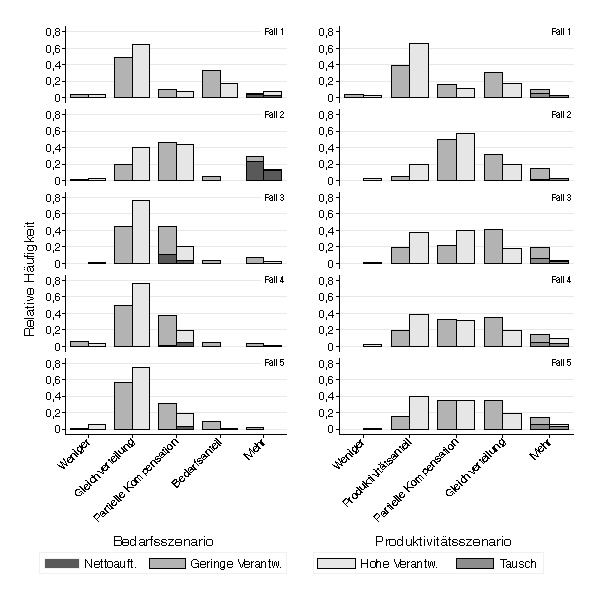
\includegraphics[width=0.99\linewidth]{figure_9.pdf}
\end{figure}

Im linken Paneel zeigt sich, dass Gleichverteilung, partielle Kompensation und Verteilung nach Bedarfsanteil die meisten Entscheidungen im Bedarfsszenario abdecken (nämlich 89\,\% in der Kontrollgruppe und 92\,\% in der Verantwortungsgruppe).
Die Verteilung nach Bedarfsanteil ist nur im ersten Fall, in dem Person~A eine gravierende Unterversorgung erfährt, nennenswert vertreten.
Wenn Person~A für ihre Situation verantwortlich ist, verschieben sich die Entscheidungen~-- wie $\chi^{2}$-Tests zeigen~-- signifikant in Richtung Gleichverteilung (und zwar von 44\,\% zu 66\,\%).
Die dunklen Balken zeigen zusätzlich den Anteil an Entscheidungen in einer Gruppe, die auch durch ein \enquote{Nettoaufteilungsprinzip} zu erklären wären.
Bei diesem Prinzip erhält Person~A so viele Holzscheite, wie sie benötigt, zuzüglich oder abzüglich der Hälfte des Überschusses oder Defizits.
Immerhin 8\,\% der Entscheidungen in der Kontrollgruppe und 5\,\% in der Verantwortlichkeitsgruppe entsprechen diesem Prinzip; besonders ausgeprägt ist es mit 23\,\% und 12\,\% außerdem in Fall 2.

Im rechten Paneel sehen wir, dass Verteilung nach Produktivitätsanteil, partielle Kompensation sowie Gleichverteilung die meisten Entscheidungen im Produktivitätsszenario abdecken (nämlich 85\,\% in der Kontrollgruppe und 94\,\% in der Verantwortlichkeitsgruppe).
Ist Person~A hier für ihren Nachteil verantwortlich, nimmt die Gleichverteilung~-- wie $\chi^{\textrm{2}}$-Tests zeigen~-- signifikant ab (und zwar von 35\,\% zu 19\,\%).
Es gibt einen nennenswerten Anteil von Teilnehmer*innen (nämlich 14\,\% und 5\,\%), die mehr als die Hälfte der Holzscheite an Person~A verteilt haben, obwohl Person~A und Person~B gleich viel benötigen und Person~A überdies weniger geschlagen hat als Person~B; die dunkel eingefärbten Balken repräsentieren hier dieses \enquote{Tauschprinzip}.

\begin{figure}[t]\label{fig:abbildung_10}
   \center
   \caption{Konsistenz der Verteilungsentscheidungen im Bedarfsszenario (linkes Paneel)
und Produktivitätsszenario (rechtes Paneel) nach Gruppe}
   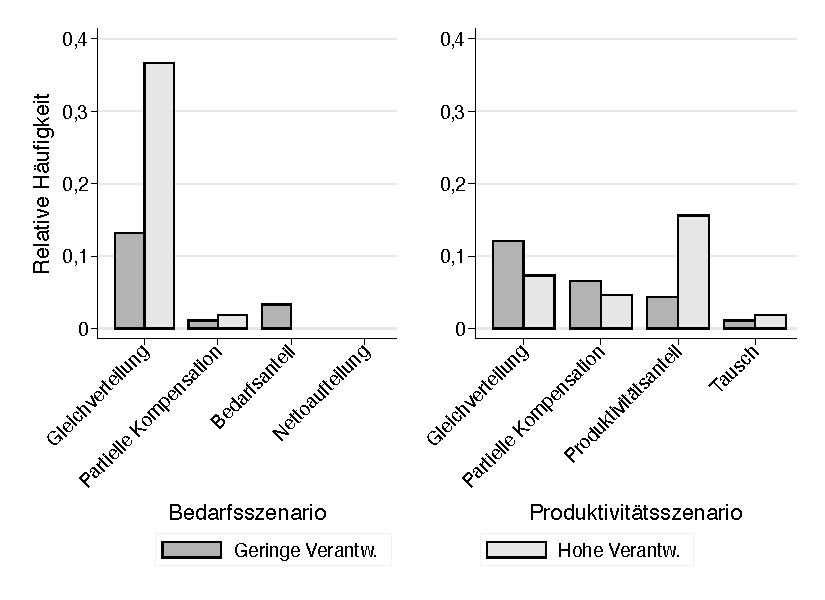
\includegraphics[width=0.99\linewidth]{figure_10.pdf}
\end{figure}

Abschließend werfen wir einen Blick darauf, wie konsistent unsere Teilnehmer*innen ihre Entscheidungen getroffen haben.
Abbildung~\ref{fig:abbildung_10} zeigt hierzu diejenigen vier Prinzipien, die in den beiden Szenarien jeweils am häufigsten gewählt wurden.
Im Bedarfsszenario sind das Gleichverteilung, partielle Kompensation, Verteilung entsprechend Bedarfsanteil sowie die Nettoaufteilung, während es im Produktivitätsszenario Gleichverteilung, partielle Kompensation, Verteilung nach Produktivitätsanteil sowie das Tauschprinzip sind.

Im linken Paneel sehen wir, dass im Bedarfsszenario 17,6\,\% unserer Teilnehmer*innen aus der Kontrollgruppe sowie 38,5\,\% unserer Teilnehmer*innen aus der Verantwortlichkeitsgruppe durchgehend das gleiche Prinzip angewendet haben.
Hier zeigt sich~-- durch einen $\chi^{\textrm{2}}$-Test~--, dass in der Verantwortlichkeitsgruppe (mit 37\,\%) signifikant mehr Teilnehmer*innen die Gleichverteilung gewählt haben als in der Kontrollgruppe (mit 13\,\%).
Außerdem haben sich hier nur wenige Teilnehmer*innen durchgehend für die partielle Kompensation oder die Erfüllung des Bedarfs von Person~A entschieden, während die Nettoaufteilung hier von keinem konsistent über alle Fälle angewendet wurde.

Das rechte Paneel zeigt, dass im Produktivitätsszenario 24,2\,\% aus der Kontrollgruppe sowie 29,4\,\% aus der Verantwortlichkeitsgruppe durchgehend das gleiche Prinzip angewendet haben.
Hier haben 12\,\% in der Kontrollgruppe und 7\,\% in der Verantwortlichkeitsgruppe durchgehend die Gleichverteilung gewählt.
Zwischen den Gruppen gibt es keine nennenswerten Unterschiede hinsichtlich der Verwendung von Gleichverteilung, partieller Kompensation oder Tauschprinzip.
Die Verteilung entsprechend des Produktivitätsanteils von Person~A ist dafür in der Verantwortlichkeitsgruppe signifikant häufiger gewählt worden.

Es zeigt sich also, dass die Zahl der Teilnehmer*innen, die durchgehend nach dem gleichen Prinzip verteilen, auffällig niedrig ist, wobei unter Umständen zu vermuten wäre, dass unsere Teilnehmer*innen sich an die unterschiedlichen Rahmenbedingungen der einzelnen Fälle anpassen.
Außerdem fallen die individuellen Entscheidungen weniger zugunsten von Person~A aus, wenn diese für ihren Nachteil verantwortlich ist, was wir als weiteren Beleg für unsere Verantwortlichkeitshypothese werten.
Bei diesem Blick auf die individuellen Entscheidungen hat sich außerdem gezeigt, dass unsere anfänglichen Beobachtungen zum durchschnittlichen Anteil oder der durchschnittlichen Abweichung weniger das Resultat einer bloß abgeschwächten Bereitschaft sind, Person~A zu kompensieren, sondern eher daher rühren, dass einige Teilnehmer*innen sich dafür entscheiden, diese Person gar nicht zu kompensieren.

Wir können festhalten, dass wir Belege für unsere Kompensationshypothese ebenso wie für unsere Verantwortlichkeitshypothese gefunden haben: Bei den Verteilungen unserer Teilnehmer*innen spielt das Bedarfsprinzip eine deutliche Rolle.
Die schlechtergestellte Person, die also entweder mehr benötigt oder weniger zur verfügbaren Menge beigetragen hat, wird für ihre schlechte Position teilweise kompensiert.
Im Durchschnitt bekommt sie mehr zugeteilt, als sie selbst produziert hat, weil ihr Bedarf in den meisten Fällen (mit Ausnahme von Fall 1 im Produktivitätsszenario) über dieser selbst geschlagenen Menge Holz liegt.
Dabei gilt das Bedarfsprinzip aber nicht bedingungslos; vielmehr wird es gegen das Leistungsprinzip abgewogen.
Die Bereitschaft zur Kompensation sinkt außerdem, wenn die schlechtergestellte Person selbst verantwortlich für ihre Situation ist, was an Debatten aus dem Glücks\-egalitarismus erinnert: Der aus \enquote{brute luck} erwachsene Nachteil der genetisch veranlagten Krankheit qualifiziert stärker zur Kompensation als der aus \enquote{option luck} resultierende Nachteil \citep{dworkin_sovereign_2000}.

Im Bedarfsszenario steigt der relative Anteil von Person~A am Gesamtbedarf von Fall zu Fall an; im Produktivitätsszenario wiederum sinkt der relative Anteil von Person~A an der Gesamtproduktivität von Fall zu Fall. Für unsere Anteiligkeitshypothese haben wir Belege gefunden: Der Anteil, den unsere Teilnehmer*innen Person~A zusprechen, hängt~-- wie wir gesehen haben~-- auch vom Bedarfs- beziehungsweise Produktivitätsanteil ab und ist damit wohl ganz im Sinne der aristotelischen Proportionalität \citep[167--172, 1131\,a--1132\,b]{aristoteles_nikomachische_2006}.

Außerdem fällt die Kompensation von Person~A im Produktivitätsszenario häufig niedriger aus als im Bedarfsszenario, unsere Symmetriehypothese muss also verworfen werden.
Unproduktiver zu sein, scheint unseren Teilnehmer*innen also weniger kompensationswürdig, als bedürftiger zu sein.
Hier zählen für sie also nicht nur die nackten Zahlen, sondern auch der Kontext, in den sie gebettet sind.


%%%%%%%%%%%%%%%%
% BEDARFSARTEN %
%%%%%%%%%%%%%%%%
\section{Bedarfsarten}\label{sec:bedarfsarten}
Unsere beiden abschließenden Studien bauen auf der Vignette auf, die in Abschnitt~\ref{sec:verantwortung} eingeführt wurde.
Wieder haben wir unseren Teilnehmer*innen hypothetische Personen vorgestellt, die Feuerholz benötigen würden, wobei wir dieses Mal variiert haben, \textit{wofür} das Holz gebraucht wird.
Insgesamt wurden unseren Teilnehmer*innen dafür vier verschiedene Bedarfsarten präsentiert.
Während sie in Studie~1 bewerten mussten, wie wichtig ihnen die Erfüllung des jeweiligen Bedarfs erscheint (Abschnitt~\ref{sec:bedarfsarten_1}), mussten sie in Studie~2~-- ähnlich wie in der Verantwortlichkeitsstudie (Abschnitt~\ref{sec:verantwortung})~-- eigene Verteilungsentscheidungen treffen (Abschnitt~\ref{sec:bedarfsarten_2}).\footnote[][-3cm]{Diese beiden Studien liegen als Arbeitspapier vor \citep{bauer_kinds_2023}. Auf eine weitere Studie \citep{bauer_deeds_nd}, die im Wesentlichen die Ergebnisse aus Abschnitt~\ref{sec:verantwortung} repliziert und ein erstes Mal die Idee der vier Bedarfsarten einführt, wird an dieser Stelle aus Platzgründen nicht weiter eingegangen.}
Obwohl die Rolle verschiedener Bedarfsarten stellenweise in der Philosophie, der Motivationspsychologie oder der Experimentellen Ökonomie verhandelt wird, waren uns keine Studien bekannt, in denen systematisch der Einfluss verschiedener Bedarfsarten auf Verteilungsentscheidungen von unparteiischen Beobachter*innen untersucht wird.
Die nachfolgend dargestellten Studien sollten einen kleinen Teil dazu beitragen, diese Lücke zu schließen.


%%%%%%%%%%%%%%%%%%
% BEDARFSARTEN 1 %
%%%%%%%%%%%%%%%%%%
\subsection{Studie~1}\label{sec:bedarfsarten_1}
Zu Beginn von Studie~1 erhielten unsere Teilnehmer*innen eine Übersicht, in der ihnen die vier verschiedenen Bedarfsarten vorgestellt wurden, um die sich die Studie im weiteren Verlauf drehen sollte.
Hierzu wurden sie gebeten, sich vier hypothetische Personen vorzustellen, die aus unterschiedlichen Gründen Feuerholz benötigen.
In zufälliger Reihenfolge wurden ihnen zu diesen vier Personen untereinander kurze Vignetten präsentiert, in denen die jeweiligen Gründe beschrieben wurden.

\begin{marginfigure}[-6.3cm]
   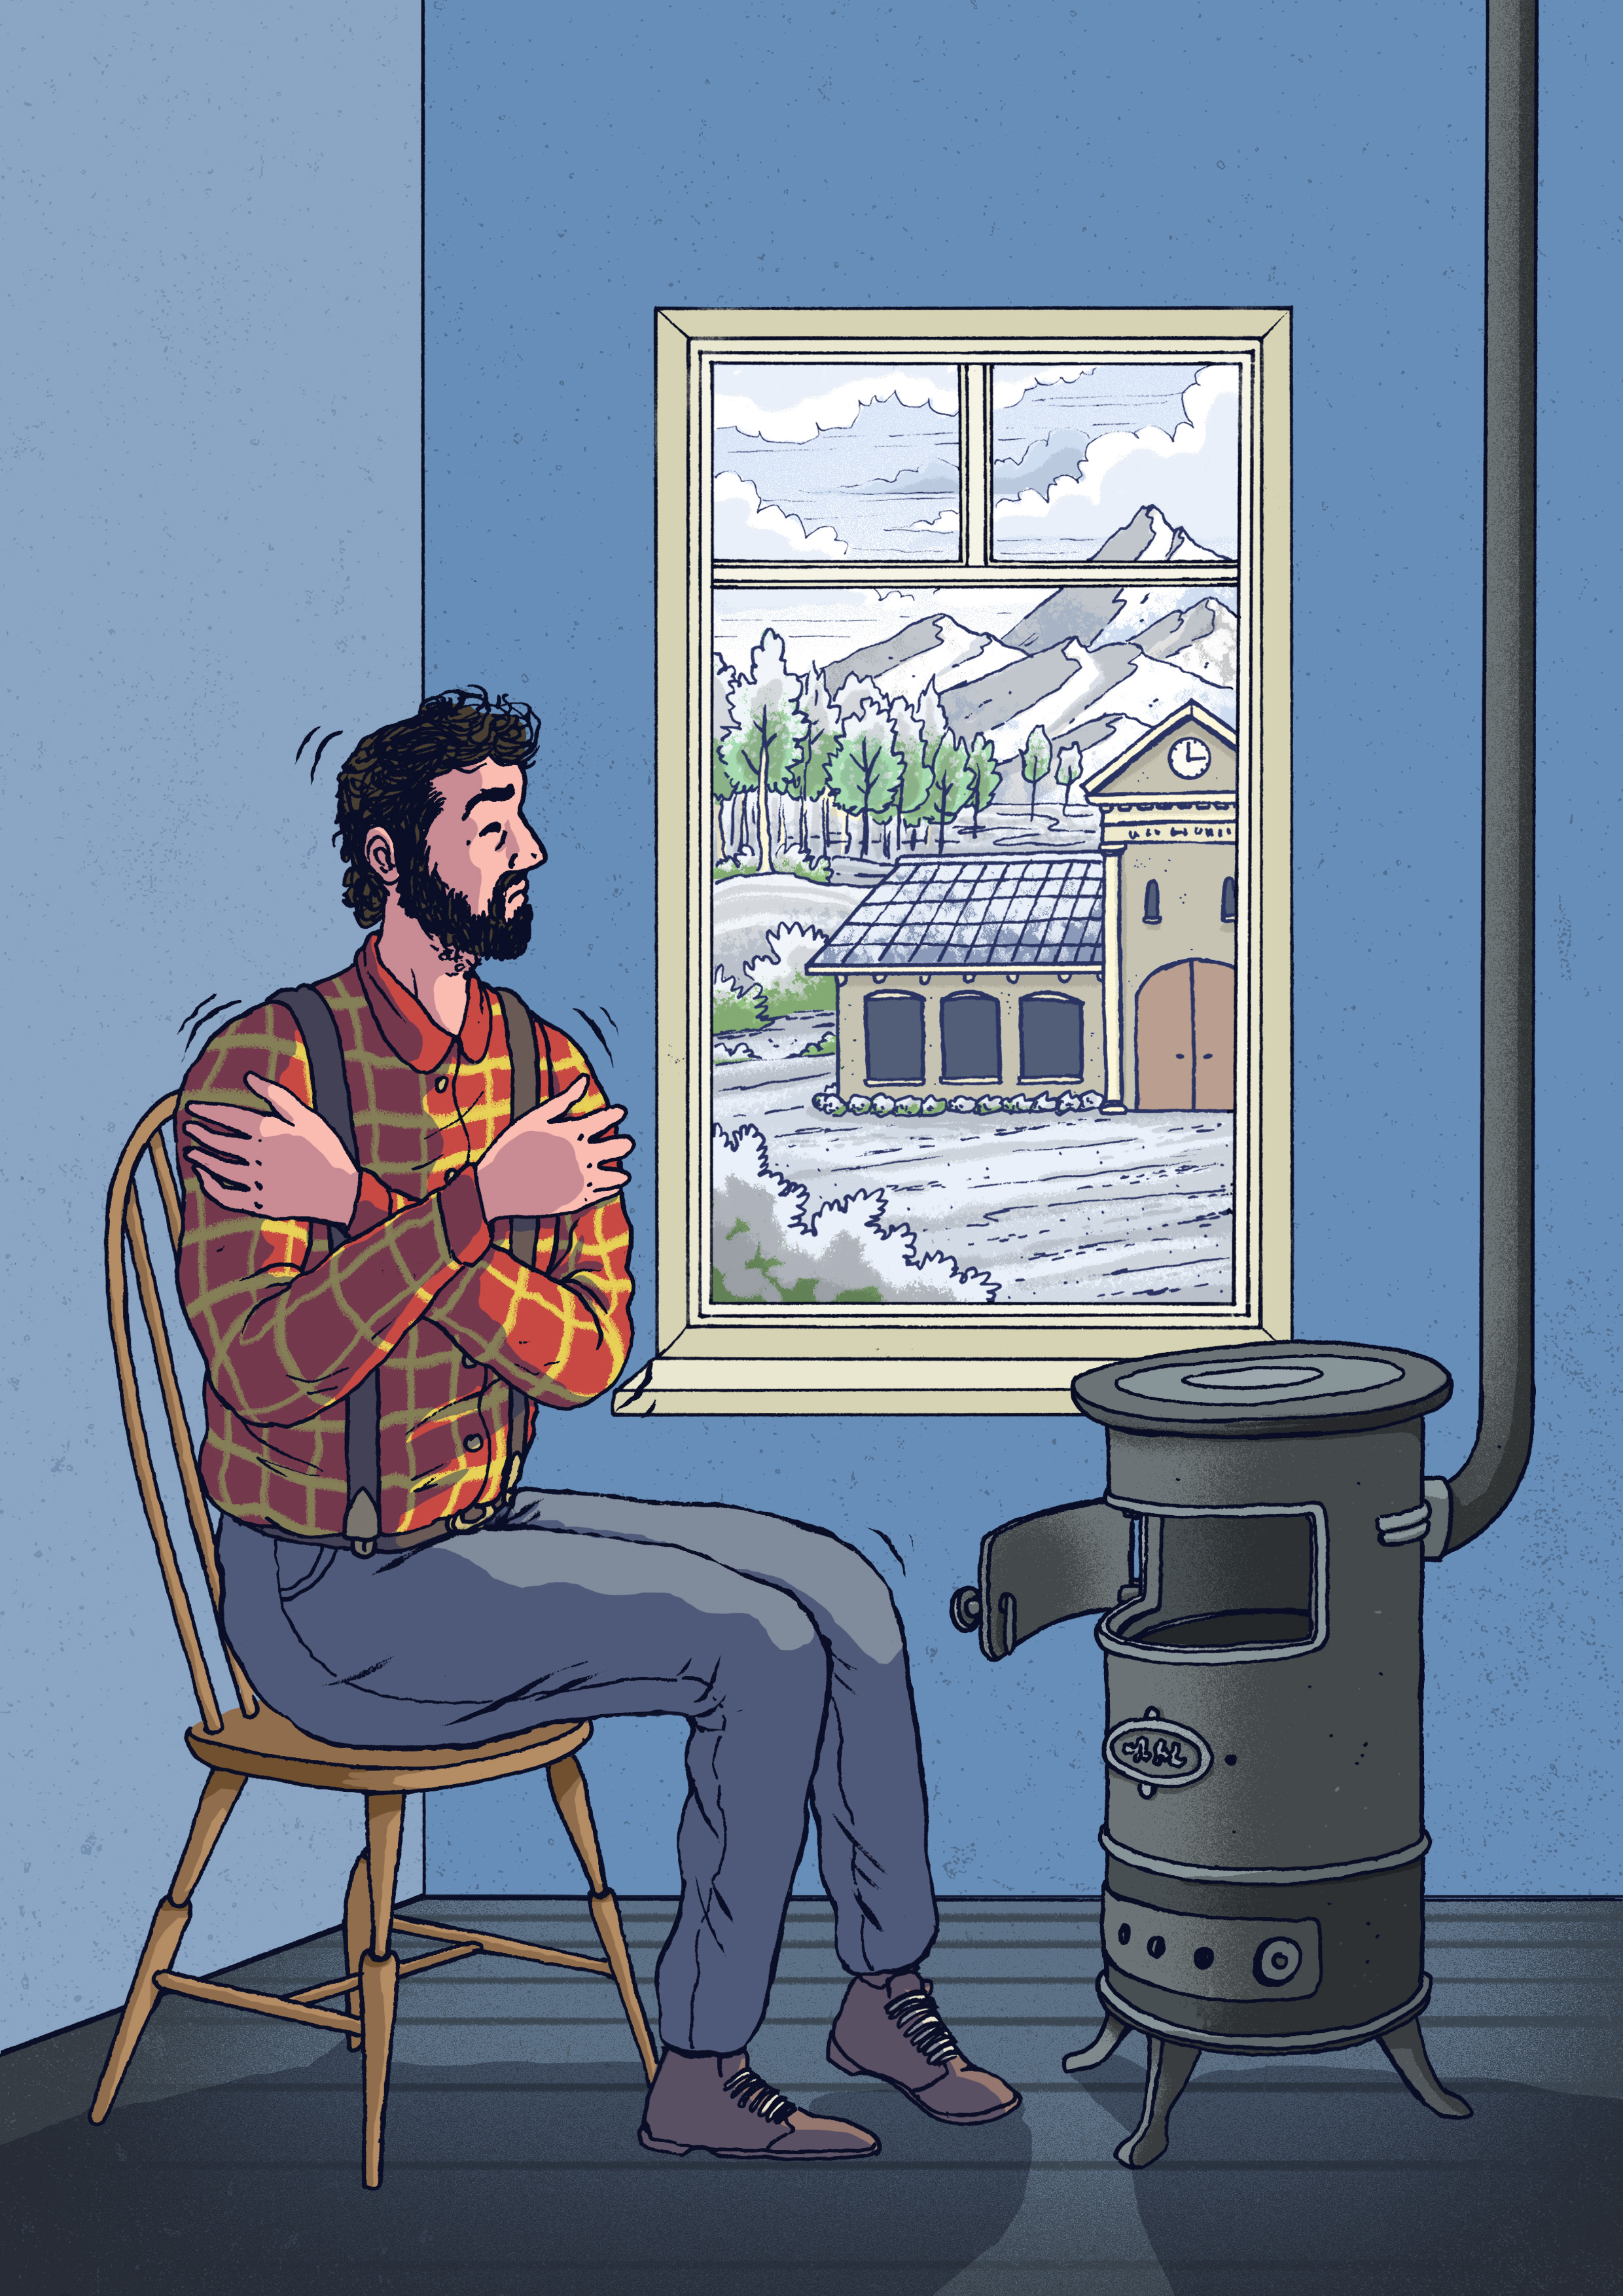
\includegraphics[width=\linewidth]{figure_11.jpg}
   \caption{Illustration Überleben}
   \label{fig:abbildung_11}
\end{marginfigure}

\begin{marginfigure}[-0.1cm]
   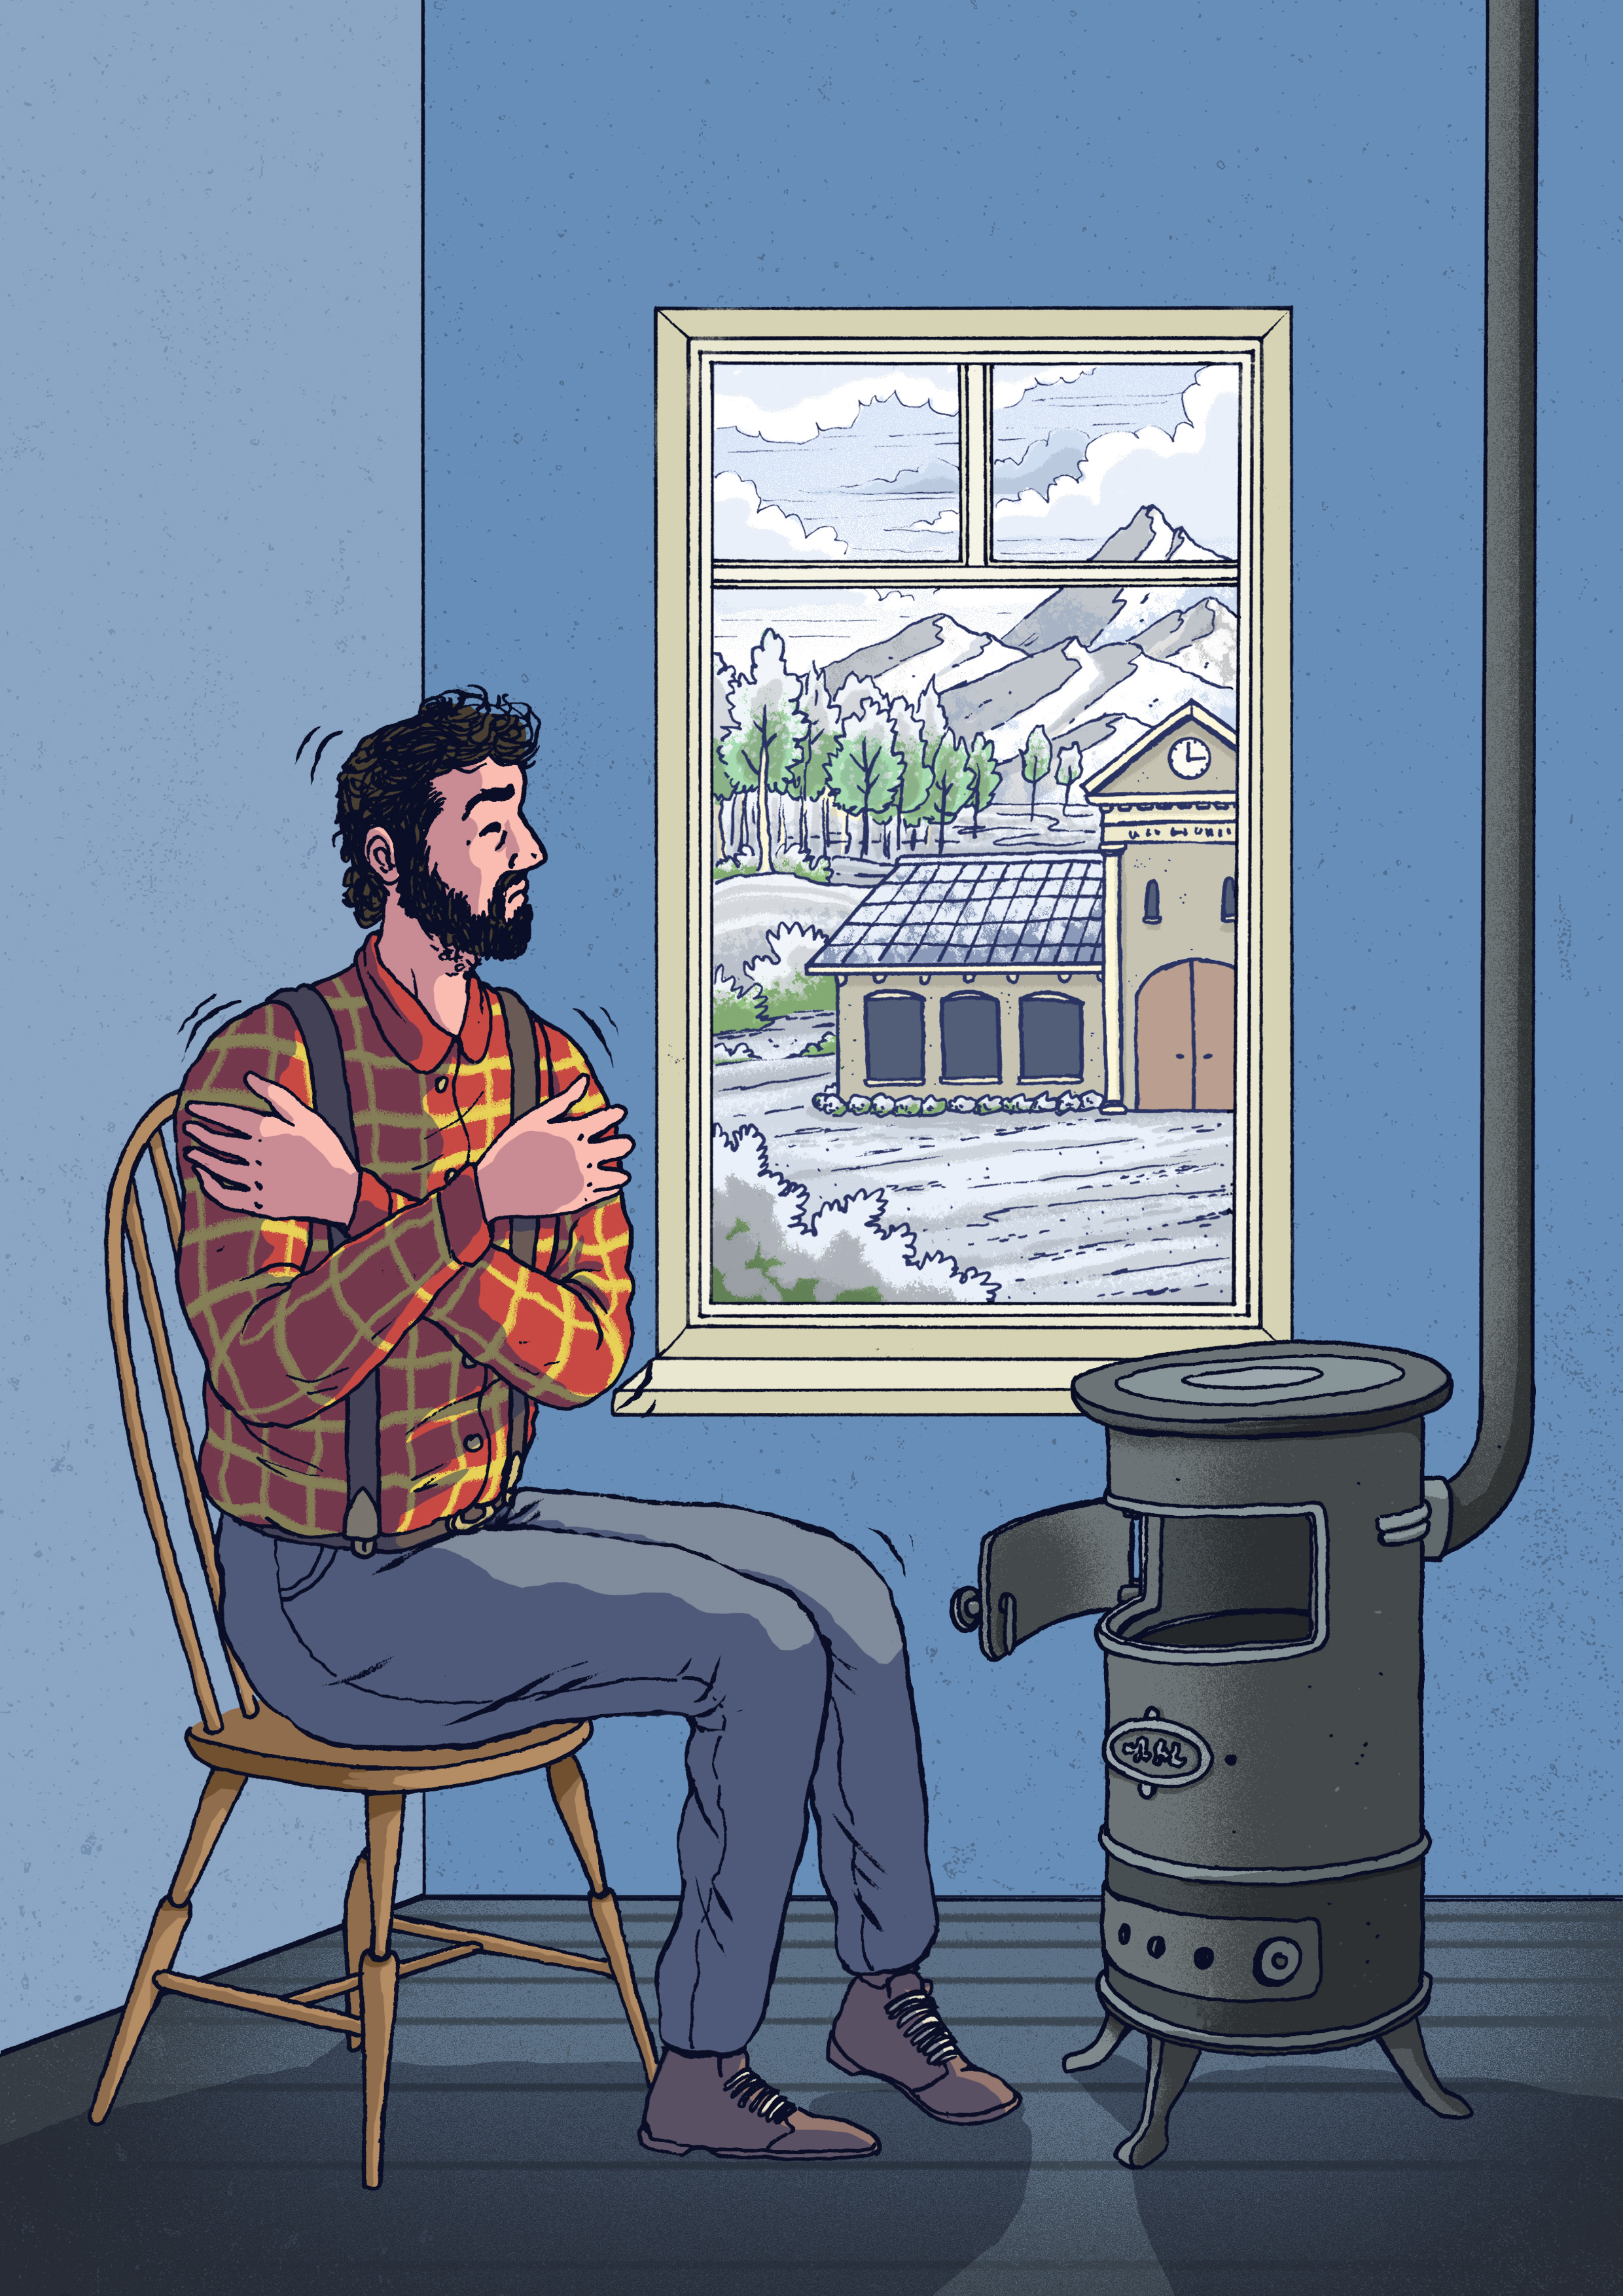
\includegraphics[width=\linewidth]{figure_12.jpg}
   \caption{Illustration Würde}
   \label{fig:abbildung_12}
\end{marginfigure}

Eine der Personen würde das Holz zum Überleben benötigen.
In der entsprechenden Vignette wurden unsere Teilnehmer*innen darüber informiert, dass diese Person das Holz zum Heizen ihrer Hütte benötigen würde, um im kommenden Winter nicht lebensbedrohlich zu erkranken.
Eine andere Person würde das Holz benötigen, um in Würde leben zu können.
Zwar würde sie über genügend Holz verfügen, um den kommenden Winter zu überleben, würde aber zusätzliches Heizmaterial benötigen, um~-- ähnlich wie in der Verantwortlichkeitsstudie (Abschnitt~\ref{sec:verantwortung})~-- zu verhindern, dass es in ihrer Hütte während des kommenden Winters ungebührlich kalt wird.
Von einer dritten Person würde das Holz zur gesellschaftlichen Teilhabe benötigt, da es gängige Praxis sei, sich während des Winters in einem Gemeindezentrum zu treffen, wobei jeder angehalten wäre, Holz mitzubringen, mit dem während der Zusammenkunft geheizt werden kann.
Schließlich gab es eine Person, die das Holz für eine gewisse Art von Autonomie benötigen würde.
Sie würde ihre Freizeit damit verbringen, in ihrem Atelier Kunst zu schaffen.
Da sie ihr Atelier ausschließlich mit Holz heizen würde, bräuchte sie entsprechendes Brennmaterial also, um in dieser Hinsicht gewissermaßen autonom über ihre Freizeitgestaltung entscheiden zu können.
Um die Unterscheidung möglichst einfach und die verschiedenen Bedarfsarten möglichst salient zu machen, wurde jede Vignette von einer Illustration begleitet, die der niederländische Künstler Douwe Dijkstra angefertigt hat (siehe Abbildungen ~\ref{fig:abbildung_11} bis~\ref{fig:abbildung_14}).

Anschließend wurde unseren Teilnehmer*innen jede Bedarfsart in der gleichen zufälligen Reihenfolge auf vier einzelnen Seiten vorgelegt.
Im Zentrum jeder Seite stand dabei die jeweilige Illustration, unter der ein einzelner Satz noch einmal die dargestellte Bedarfsart zusammenfasste.
Darunter wiederum wurden unsere Teilnehmer*innen gebeten, ihre Einschätzung auf einer Skala von 1 (\enquote{benötigt das Holz überhaupt nicht}) bis 7 (\enquote{benötigt das Holz unbedingt}) hinsichtlich der Frage abzugeben, wie sehr die Person das Holz im jeweiligen Fall benötigen würde.

\begin{marginfigure}[6.2cm]
   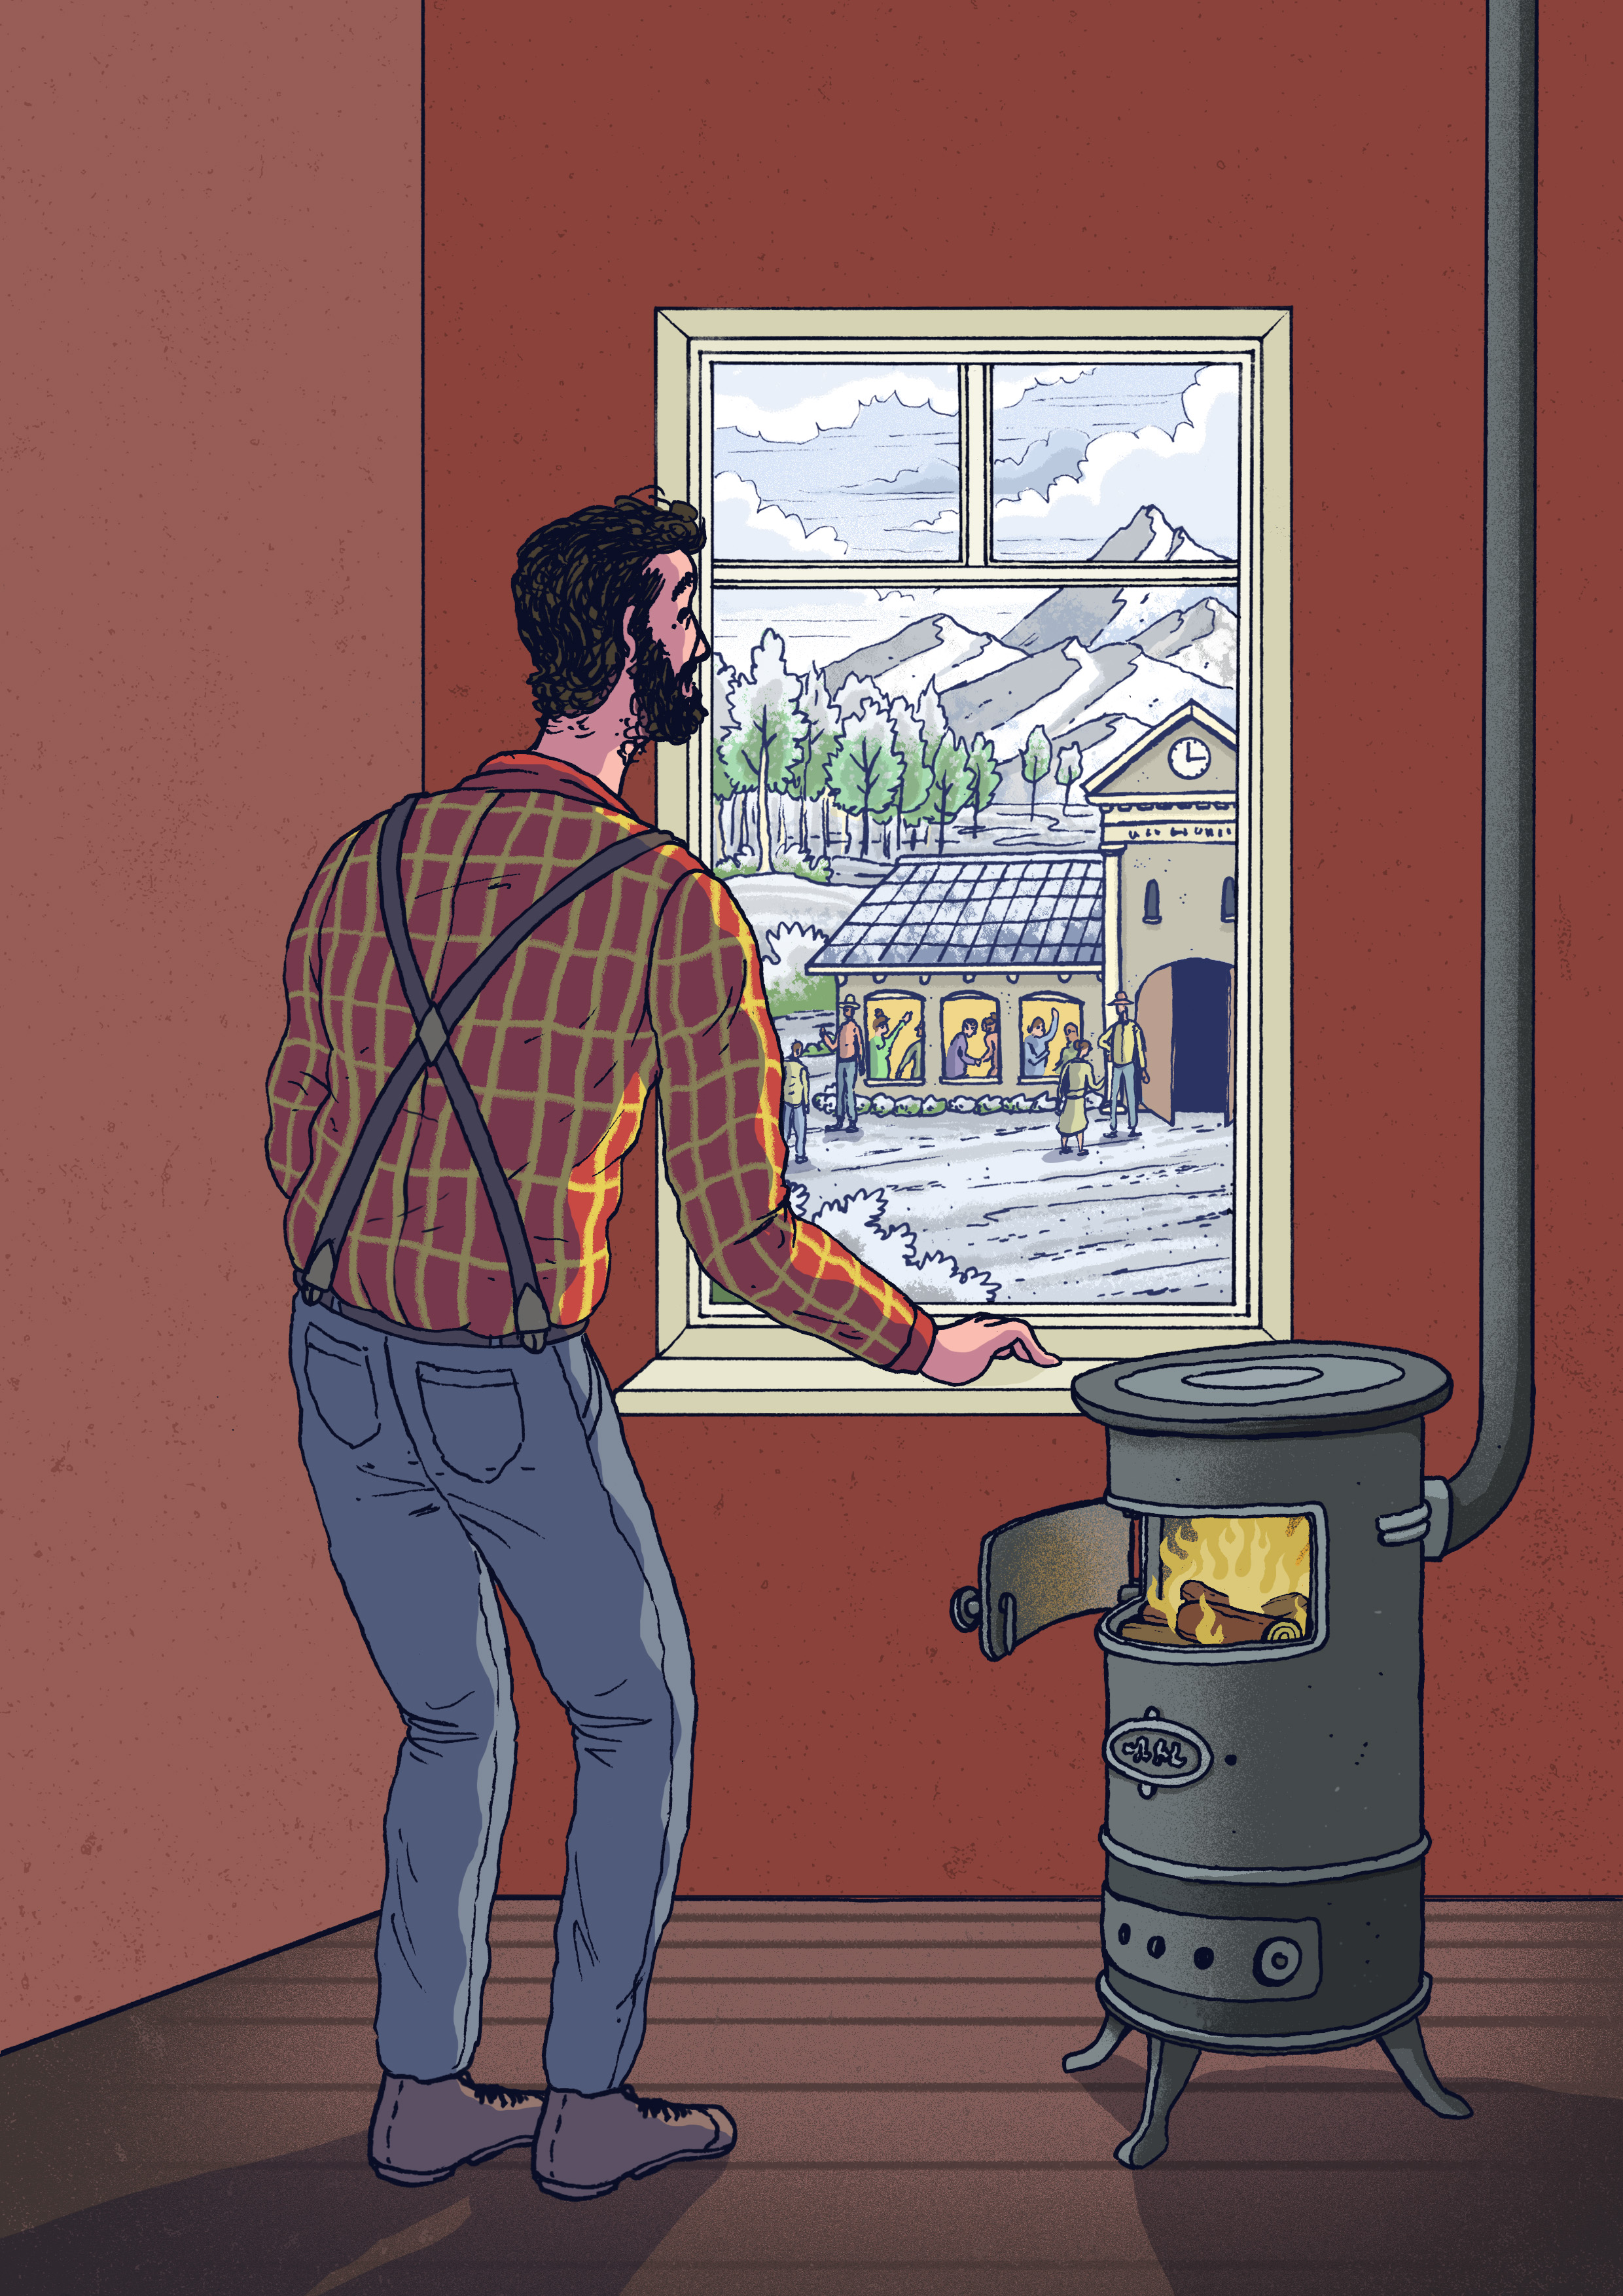
\includegraphics[width=\linewidth]{figure_13.jpg}
   \caption{Illustration Teilhabe}
   \label{fig:abbildung_13}
\end{marginfigure}

\begin{marginfigure}[-0.1cm]
   
\includegraphics[width=\linewidth]{figure_14.jpg}
   \caption{Illustration Autonomie}
   \label{fig:abbildung_14}
\end{marginfigure}

Diese Studie wurde, wie schon die vorherige, in \textit{oTree} umgesetzt.
Durchgeführt wurde sie im Februar 2021; unsere Teilnehmer*innen wurden abermals von \textit{respondi} rekrutiert, wieder stratifiziert nach Geschlecht (weiblich: 50,0\,\%, männlich: 50,0\,\%), Alter (18--29 Jahre: 21,0\,\%, 30--39 Jahre: 18,0\,\%, 40--49 Jahre: 19,0\,\%, 50--59 Jahre: 24,0\,\%, 60--69 Jahre: 18,0\,\%) sowie Nettoäquivalenzhaushaltseinkommen (0--1.099 Euro: 16,0\,\%, 1.100--1.499 Euro: 23,0\,\%, 1.500--1.999 Euro: 23,0\,\%, 2.000--2.599 Euro: 19,0\,\%, 2.600 und mehr Euro: 19,0\,\%).
Auch in dieser Studie wurden unseren Teilnehmer*innen insgesamt drei Verständnisfragen gestellt, von denen sie mindestens zwei richtig beantworten mussten, um nicht aus der Studie ausgeschlossen zu werden.
Insgesamt haben 100 Teilnehmer*innen die Studie erfolgreich abgeschlossen und dafür einen Festbetrag von 4,15 Euro für ihre etwa fünfzehnminütige Teilnahme erhalten.

Vor dem Hintergrund der philosophischen Literatur sind wir davon ausgegangen, dass unsere Teilnehmer*innen alle vier Bedarfsarten zu einem gewissen Grad anerkennen sollten, dass ihre Einschätzung davon, wie wichtig deren Erfüllung ist, jedoch von Bedarfsart zu Bedarfsart schwanken würde.
Diejenigen Bedarfsarten, die in der Theorie \enquote{basaler} sind, würden~-- so unsere Vermutung~-- im Durchschnitt eine höhere Einschätzung erhalten als weniger basale Bedarfsarten.
Mit Blick auf die durchschnittliche Einschätzung sind wir davon ausgegangen, dass die Bewertung am höchsten sein würde für die Kategorie Überleben, gefolgt von Würde, Teilhabe und Autonomie, was sich für die Mittelwerte (\textit{M}) also darstellen ließe wie in (\ref{eq:mittelwert}).

\begin{equation}\label{eq:mittelwert}
   M_{\ddot{U}berleben}>M_{W\ddot{u}rde}>M_{Teilhabe}>M_{Autonomie}
\end{equation}

In Abbildung~\ref{fig:abbildung_15} sehen wir die Mittelwerte der Einschätzungen unserer Teilnehmer*innen für die vier Bedarfsarten.
Hier wird deutlich, dass die Bedeutung des Überlebens im Mittel tatsächlich am höchsten eingeschätzt wird ($M = \textrm{6,830}$), gefolgt von Würde ($M = \textrm{5,990}$) sowie~-- nach einem deutlichen Abfall~-- Teilhabe ($M = \textrm{4,051}$) und Autonomie ($M = \textrm{3,300}$).
Dieser Eindruck wird zusätzlich von einer einfaktoriellen Varianzanalyse gestützt, aus der hervorgeht, dass alle paarweisen Vergleiche, die sich zwischen den vier Bedarfsarten anstellen lassen, signifikante Differenzen in der Bewertung aufweisen.
Wir können also davon ausgehen, dass die Erfüllung der verschiedenen Bedarfsarten von unseren Teilnehmer*innen als unterschiedlich bedeutend eingeschätzt wurde, wobei die gefundene Hierarchie mit der theoretisch angenommenen übereinstimmt.


%%%%%%%%%%%%%%%%%%
% BEDARFSARTEN 2 %
%%%%%%%%%%%%%%%%%%
\subsection{Studie~2}\label{sec:bedarfsarten_2}
Auch unsere zweite Studie baute auf der in Abschnitt~\ref{sec:verantwortung} vorgestellten Vignette auf, wobei wir hier~-- wie sich gleich zeigen wird~-- näher an der ursprünglichen Form sind als in unserer ersten Bedarfsartenstudie.
Wieder haben unsere Teilnehmer*innen eine Geschichte vorgelegt bekommen, in der es zwei hypothetische Personen gab, die einen Bedarf an Feuerholz aufwiesen und die zu dessen Deckung Holz im gemeindeeigenen Wald schlagen durften.
Diesmal haben wir variiert, wofür die beiden dieses Holz jeweils benötigen würden.
Neben dem grundlegenden Hintergrund unserer Vignette wurden die Teilnehmer*innen daher wie in unserer ersten Bedarfsartenstudie darüber informiert, dass im Rahmen dieser Studie von insgesamt vier verschiedenen Bedarfsarten die Rede sein würde.
Person~A oder Person~B könnten das Holz~-- wie oben~-- benötigen, um den kommenden Winter zu überleben, um während des Winters in würdevollen Verhältnissen zu leben, um während des Winters am gesellschaftlichen Leben teilhaben zu können oder um während des Winters autonom über ihre Freizeitgestaltung entscheiden zu können.
Wie in der ersten Bedarfsartenstudie wurde jede Beschreibung einer Bedarfsart zusätzlich von einer Illustration begleitet (siehe Abbildungen~\ref{fig:abbildung_11} bis~\ref{fig:abbildung_14}), in der die betroffene Person in einer Situation zu sehen war, in der sie ihren jeweiligen Bedarf nicht erfüllen konnte.

\begin{figure}[t]\label{fig:abbildung_15}
   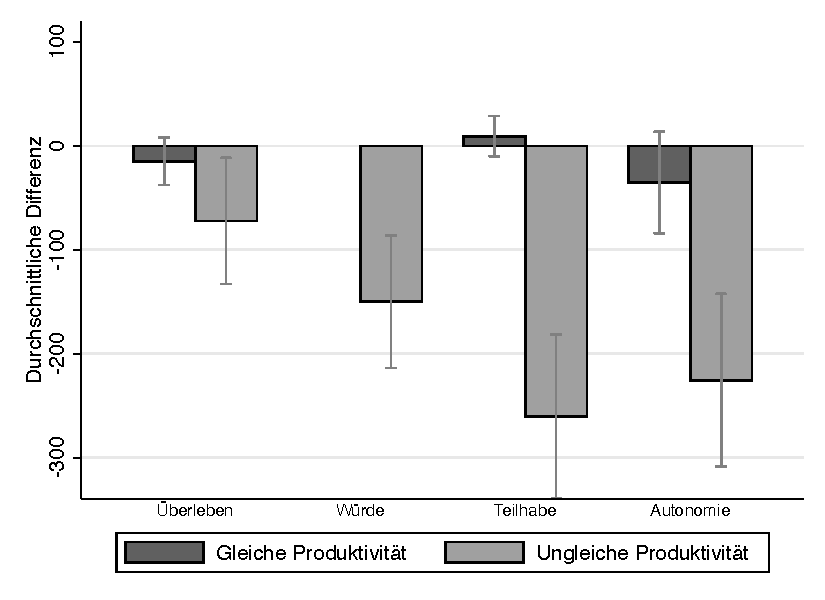
\includegraphics[width=0.99\linewidth]{figure_15.pdf}
   \caption{Mittelwerte der zugeschriebenen Bedeutung der vier Bedarfsarten}
\end{figure}

Nachdem unsere Teilnehmer*innen mit den verschiedenen Bedarfsarten vertraut gemacht worden waren, legten wir ihnen eine Reihe von Fällen vor, wobei wir zwischen gepaarte Fällen und gemischten Fällen unterschieden.
Bei \textit{gepaarten Fällen} wiesen Person~A und Person~B jeweils die gleiche Bedarfsart auf; dementsprechend gab es vier gepaarte Fälle.
Bei \textit{gemischten Fällen} wiederum wiesen Person~A und Person~B jeweils unterschiedliche Bedarfsarten auf; hier gab es dementsprechend insgesamt sechs verschiedene Kombinationen (siehe Tabelle~\ref{tab:kombinationen}).

Die Aufgabe unserer Teilnehmer*innen war es~-- wie in unserer Verantwortlichkeitsstudie (Abschnitt~\ref{sec:verantwortung})~--, das zur Verfügung stehende Holz in einer Reihe von Fällen so zwischen Person~A und Person~B aufzuteilen, dass eine in ihren Augen möglichst gerechte Verteilung erreicht wird.
Dabei waren unsere Teilnehmer*innen~-- zumindest in den gemischten Fällen~-- gezwungen, Abwägungen hinsichtlich der Bedeutsamkeit der zwei in einem Fall jeweils präsentierten Bedarfsarten vorzunehmen, da die zur Verfügung stehende Menge an Holz nur ausreichen würde, um den Bedarf einer der beiden Personen gerade eben zu decken (mit 1.000 Holzscheiten war die von Person~A und Person~B insgesamt geschlagene und damit zur Verteilung stehende Holzmenge dabei über alle Fälle konstant).
Jeder Fall wurde auf einer separaten Seite dargestellt, in deren Mitte zwei nebeneinanderstehende Illustrationen die Bedarfsarten von Person~A und Person~B zeigten.
Unter jeder Illustration beschrieb ein knapper Satz noch einmal, wofür die Person das Holz jeweils benötigen würde.
Darunter wiederum konnten die Teilnehmer*innen dann angeben, wieviel Holz Person~A und Person~B in diesem Fall jeweils erhalten sollten, wobei wieder alle zur Verfügung stehenden Holzscheite verteilt werden mussten.

\begin{table}[t]
   \caption{Kombinationen von Bedarfsarten für gemischte Fälle}\label{tab:kombinationen}
   \begin{center}
   \begin{tabular}{lcccccc}
   \hline
   Fall       & 1        & 2        & 3        & 4        & 5        & 6        \\
   \hline\hline
   Person~A   & Überl.   & Überl.   & Überl.   & Würde    & Würde    & Teilh.   \\
   Person~B   & Würde    & Teilh.   & Auton.   & Teilh.   & Auton.   & Auton.   \\
   \hline
   \end{tabular}
   \end{center}
\end{table}

Diese Fälle wurden den Teilnehmer*innen in zwei aufeinanderfolgenden Szenarien präsentiert.
Im \textit{Szenario gleicher Produktivität} hatten Person~A und Person~B jeweils 500 Holzscheite geschlagen, im \textit{Szenario ungleicher Produktivität} hatte Person~A nur 200, Person~B dafür 800 Holzscheite geschlagen.
Jedes dieser Szenarien enthielt sieben Fälle; einen zufällig ausgewählten gepaarten Fall (der dann in beiden Szenarien präsentiert wurde) sowie die sechs gemischten Fälle.
Die Reihenfolge der beiden Szenarien sowie der Fälle innerhalb dieser Szenarien und der Position von Person~A und Person~B auf jedem Bildschirm wurden für alle Teilnehmer*innen zufällig ausgewählt.

Um einen möglichen Indikator dafür zu haben, ob eventuelle Effekte auf Spezifika der Formulierungen zurückgehen könnten, wurde dieser Aufbau außerdem mit zwei getrennten Gruppen von Teilnehmer*innen durchgeführt.
Eine Gruppe erhielt die Beschreibungen in einer \textit{Vermeidungsformulierung}, eine Gruppe in einer \textit{Ermöglichungsformulierung}.
Bei der Vermeidungsformulierung stand dabei die Abwendung von unerwünschten Konsequenzen im Vordergrund, während die Ermöglichungsformulierung die Realisierung wünschenswerter Zustände betonte.

Für unsere Analyse haben wir die Differenz berechnet zwischen dem Holz, das in einem Fall Person~A (in den gemischten Fällen also der Person mit der grundlegenderen Bedarfsart) zugesprochen wurde, sowie dem Holz, das in diesem Fall Person~B (in den gemischten Fällen also der Person mit einer weniger grundlegenden Bedarfsart) zugesprochen wurde.
Diese Differenz wird im Folgenden als $\Delta$ bezeichnet.
Wenn Person~A beispielsweise das Holz zum Überleben benötigt, während Person~B es zur autonomen Freizeitgestaltung benötigt, ergibt sich die Differenz $\Delta_{\ddot{U}berl.-Auton.}$  wie in (\ref{eq:differenz}), indem man die Menge, die Person~B zugesprochen bekommt ($\gamma_{B}$), von der Menge abzieht, die Person~A zugesprochen bekommt ($\gamma_{A}$).

\begin{equation}\label{eq:differenz}
   \Delta_{\ddot{U}berl.-Auton.}=\gamma_{A}-\gamma_{B}
\end{equation}

Vor dem Hintergrund der Literatur sowie der Ergebnisse unserer ersten Bedarfsartenstudie sind wir davon ausgegangen, dass den vier Bedarfsarten unterschiedliches Gewicht beigemessen werden sollte, dass also in Fällen, in denen Person~A und Person~B verschiedene Bedarfsarten zu decken haben, derjenigen Person mehr Holz zugesprochen wird, deren Bedarf als \enquote{grundlegender} wahrgenommen wird (was wir im Folgenden die Hierarchiehypothese nennen).
Wir haben dementsprechend erwartet, eine Hierarchie der Bedarfsarten zu beobachten, wobei Überleben, Würde, Teilhabe und Autonomie in dieser Reihenfolge als jeweils weniger grundlegend wahrgenommen werden sollten und sich diese Abstufung auch in den Differenzen widerspiegeln sollte.
Ausgehend von der Differenz der beiden in der Theorie am weitesten voneinander entfernten Bedarfsarten ließe sich wie in (\ref{eq:hierarchie}) beispielsweise annehmen, dass die Differenz zwischen Überleben und Autonomie größer ist als jene zwischen Überleben und Teilhabe, die wiederum größer ist als jene zwischen Überleben und Würde.

\begin{equation}\label{eq:hierarchie}
   \Delta_{\ddot{U}berl.-Auton.}>\Delta_{\ddot{U}berl.-Teil.}>\Delta_{\ddot{U}berl.-W\ddot{u}rde}
\end{equation}

Da es sich bei jeder Bedarfsart nichtsdestotrotz um einen legitimen Bedarf handeln sollte, sind wir ferner davon ausgegangen, dass jeder Bedarf zumindest teilweise kompensiert werden würde, dass es also nicht (oder zumindest nur selten) vorkommen sollte, dass unsere Teilnehmer*innen einer der beiden Personen sämtliches Holz zusprechen, während die andere Person leer ausgeht.

Wir sind außerdem davon ausgegangen, dass unsere Teilnehmer*innen kohärente Verteilungsentscheidungen treffen sollten (hier sprechen wir von der Kohärenz\-hypothese).
Wir nennen eine Verteilungsentscheidung kohärent, wenn sie additiv ist.
Additivität wiederum ist gegeben, wenn die Differenz zwischen zwei Bedarfsarten, die in der Theorie nicht benachbart sind, gleich den Differenzen der von ihnen umspannten Bedarfsarten ist.
Die Differenz zwischen Überleben und Teilhabe beispielsweise sollte der Differenz zwischen Überleben und Würde zuzüglich der Differenz zwischen Würde und Teilhabe entsprechen.
Wenn wir die Differenz von Überleben und Autonomie als Referenzwert nehmen, sollte beispielsweise (\ref{eq:additivitaet}) gelten.

\begin{equation}\label{eq:additivitaet}
   \begin{split}
   \Delta_{\ddot{U}berl.-Auton.} & = \Delta_{\ddot{U}berl.-Teilh.} + \Delta_{Teilh.-Auton.} \\
                                 & = \Delta_{\ddot{U}berl.-W\ddot{u}rde} + \Delta_{W\ddot{u}rde-Auton.} \\
                                 & = \Delta_{\ddot{U}berl.-W\ddot{u}rde} + \Delta_{W\ddot{u}rde-Teilh.} + \Delta_{Teilh.-Auton.}
   \end{split}
\end{equation}

Während wir davon ausgegangen sind, dass unsere Formulierungen keinen Unterschied zwischen den beiden Gruppen machen sollten (hier sprechen wir von der Formulierungshypothese), sollten die beiden Szenarien durchaus einen Effekt auf die Verteilungsentscheidungen unserer Teilnehmer*innen haben.
Im Szenario ungleicher Produktivität, in dem Person~A weniger Holz geschlagen hat als Person~B, sollte sie weniger Holz zugesprochen bekommen als im Szenario gleicher Produktivität (was wir die Produktivitätshypothese nennen).
Wir erwarten also für die Differenz zweier Bedarfsarten $\alpha$ und $\beta$, dass $\Delta$, wie in (\ref{eq:gleichheit}), im Szenario gleicher Produktivität größer ist als im Szenario ungleicher Produktivität.

\begin{equation}\label{eq:gleichheit}
   \Delta^{Gleiche\;Produktivit\ddot{a}t}_{\alpha-\beta}>\Delta^{Ungleiche\;Produktivit\ddot{a}t}_{\alpha-\beta}
\end{equation}

Diese Studie wurde erneut mit \textit{oTree} umgesetzt und im April 2021 durchgeführt.
Unsere Teilnehmer*innen wurden erneut durch \textit{respondi} rekrutiert und waren stratifiziert nach den Charakteristika Geschlecht (weiblich: 50,0\,\%, männlich: 50,0\,\%), Alter (18--29 Jahre: 21,0\,\%, 30--39 Jahre: 18,0\,\%, 40--49 Jahre: 19,0\,\%, 50--59 Jahre: 24,0\,\%, 60--69 Jahre: 18,0\,\%) sowie Nettoäquivalenzhaushaltseinkommen (0--1.099 Euro: 16,0\,\%, 1.100--1.499 Euro: 23,0\,\%, 1.500--1.999 Euro: 23,0\,\%, 2.000--2.599 Euro: 19,0\,\%, 2.600 und mehr Euro: 19,0\,\%).
Wieder hatten unsere Teilnehmer*innen im Anschluss an die Verteilaufgabe drei Kontrollfragen zu beantworten, wobei von der Studie ausgeschlossen wurde, wer mehr als eine dieser Fragen falsch beantwortet hatte.
Insgesamt 200 Teilnehmer*innen schlossen die Studie erfolgreich ab und wurden mit einem pauschalen Betrag von 5,40 Euro für etwa 30 Minuten ihrer Zeit entschädigt.

\begin{figure}[t]\label{fig:abbildung_16}
   \center
   \caption{Durchschnittliche Differenz für gepaarte Fälle nach Szenario}
   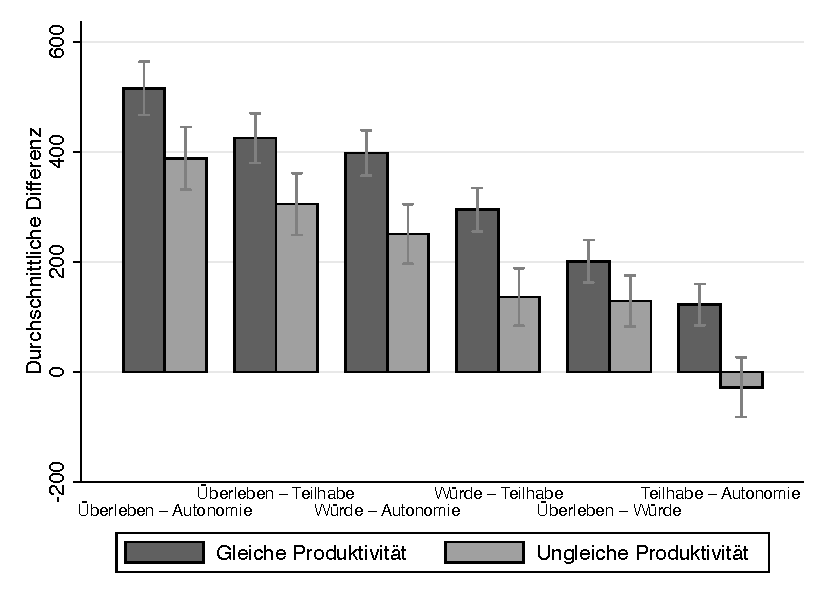
\includegraphics[width=0.99\linewidth]{figure_16.pdf}
\end{figure}

Um unsere obigen Hypothesen zu testen, haben wir die durchschnittlichen Differenzen in den Blick genommen.
Abbildung~\ref{fig:abbildung_16} zeigt diese zunächst für die Fälle gepaarter Bedarfsarten in Abhängigkeit vom Produktivitätsszenario.
Es wird deutlich, dass unsere Teilnehmer*innen das Holz im Szenario gleicher Produktivität annähernd gleich auf Person~A und Person~B aufgeteilt haben (eine Gleichverteilung würde in $\Delta = \textrm{0}$ resultieren).
Da beide Personen hier bezüglich aller präsentierten Faktoren identisch waren, scheint das auch die naheliegende Option.
Das Bild ändert sich freilich, wenn das Szenario ungleicher Produktivität in den Blick genommen wird, in dem Person~A deutlich weniger Holz geschlagen hat als Person~B.
Dementsprechend hat Person~A hier auch~-- ganz im Sinne der Produktivitätshypothese~-- weniger Holz von unseren Teilnehmer*innen zugesprochen bekommen als Person~B.
Der quantitative Unterschied scheint dabei abhängig zu sein von der jeweiligen Bedarfsart des Paares, was in Richtung unserer Hierarchiehypothese deutet.
Benötigen beide das Holz zum Überleben, hat die geringere Produktivität von Person~A einen kaum merklichen Einfluss auf die Verteilungsentscheidungen unserer Teilnehmer*innen: Obwohl Person~A deutlich weniger Holz geschlagen hatte als Person~B, bekam sie noch immer annähernd gleich viel zugeteilt.
Der Unterschied zwischen den an Person~A und Person~B verteilten Holzscheiten wächst bei Würde und ist schließlich am ausgeprägtesten bei Teilhabe und Autonomie.
Aber selbst in diesen Fällen bekam Person~A noch deutlich mehr Holz zugesprochen, als sie selbst geschlagen hatte, wird also wie in der Verantwortlichkeitsstudie (Abschnitt~\ref{sec:verantwortung}) teilweise für ihren Nachteil kompensiert.
Außerdem zeigen Tobit-Panelregressionen, dass die Formulierung~-- der Formulierungshypothese entsprechend~-- keinen Unterschied macht.

Werfen wir als nächstes einen Blick auf die sechs Fälle gemischter Bedarfsarten.
Hier zeigt Abbildung~\ref{fig:abbildung_17} die Differenzen~-- wieder aufgeteilt nach Produktivitätsszenario~-- für die sechs möglichen Kombinationen, die aus den vier Bedarfsarten gebildet werden können.
Für jede Kombination gilt, dass die durchschnittliche Differenz im Szenario ungleicher Produktivität geringer ist als im Szenario gleicher Produktivität.
Offensichtlich geben unsere Teilnehmer*innen der Person mit dem grundlegenderen Bedarf also auch in den Fällen gemischter Bedarfsarten weniger Holz, wenn diese weniger zu der insgesamt zur Verfügung stehenden Menge beigetragen hat, was weiter für unsere Produktivitätshypothese spricht.\footnote{Der Wert von $\Delta$ steigt mit einer zunehmenden Abweichung von der Gleichverteilung zwischen Person~A und Person~B an. Erhalten beide die gleiche Anzahl an Holzscheiten, lässt sich keine Differenz feststellen, da $\Delta = \textrm{500} - \textrm{500} = \textrm{0}$. Wenn Person~A, die den grundlegenderen Bedarf aufweist, mehr als Person~B erhält, wird eine posi\-tive Differenz angezeigt, beispielsweise mit $\Delta = \textrm{600} - \textrm{400} = \textrm{200}$. Diese Differenz nimmt zu, je mehr Holz Person~A erhält, bis zu maximal $\Delta = \textrm{1.000} - \textrm{0} = \textrm{1.000}$.} Erinnern wir uns daran, dass wir die Prämisse gesetzt haben, dass 1.000 Holzscheite gerade so ausreichen würden, um den Bedarf einer der beiden Personen zu decken.
Wir können also davon ausgehen, dass dieses Muster darauf hindeutet, dass unsere Teilnehmer*innen in geringerem Maße dazu bereit sind, einen~-- wenngleich grundlegenderen~-- Bedarf zu kompensieren, wenn die Person weniger zu der zur Verfügung stehenden Menge beigetragen hat als die andere Person.

Wie schon bei den Fällen gepaarter Bedarfsarten wird auch hier im Szenario ungleicher Produktivität die weniger produktive Person nichtsdestotrotz teilweise kompensiert.
Die einzige Kombination, in der die durchschnittliche Differenz darauf hindeutet, dass die Person mit dem grundlegenderen Bedarf weniger erhält als die Person mit dem weniger grundlegenden Bedarf, ist \textit{Teilhabe\,--\,Autonomie} im Szenario ungleicher Produktivität.
Selbst hier jedoch erhält Person~A ungefähr gleich viel wie Person~B, obwohl sie wesentlich weniger produziert hat als diese.\footnote{Würde die Person nur erhalten, was sie selbst geschlagen hat, läge die Differenz bei $-\textrm{600}$, da $\Delta = \textrm{200} - \textrm{800} = -\textrm{600}$.}

Ferner sehen wir, dass die Differenzen größer sind für Kombinationen von Bedarfsarten, die in der Hierarchie nicht unmittelbar benachbart sind, wobei die Differenz am größten ist für die Kombination \textit{Überleben\,--\,Autonomie}, die alle vier Bedarfsarten umspannt, so dass Überleben und Autonomie in der postulierten Hierarchie am weitesten auseinanderliegen.
Diejenigen Kombinationen, die drei Bedarfsarten umspannen (das sind \textit{Überleben\,--\,Teilhabe} sowie \textit{Würde\,--\,Autonomie}), weisen dagegen kleinere durchschnittliche Differenzen auf.
Die kleinsten Differenzen schließlich finden wir bei jenen Kombinationen, deren Bedarfsarten in der Hierarchie unmittelbar nebeneinanderliegen (nämlich \textit{Überleben\,--\,Würde}, \textit{Würde\,--\,Teilhabe} und \textit{Teilhabe\,--\,Autonomie}), was weiter in Richtung unserer Hierarchiehypothese deutet.

\begin{figure}[t]\label{fig:abbildung_17}
   \center
   \caption{Durchschnittliche Differenz für gemischte Fälle nach Szenario}
   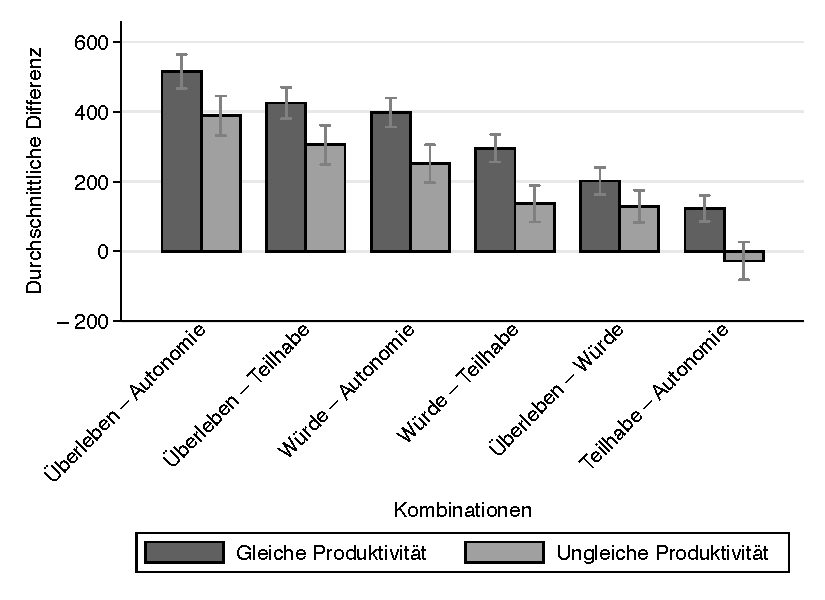
\includegraphics[width=0.99\linewidth]{figure_17.pdf}
\end{figure}

Diese Beobachtungen werden zusätzlich gestützt durch zwei Tobit-Panelregres\-sionen.
Paarweise Vergleiche der Randmittel aller Kombinationen zeigen signifikante Unterschiede für alle außer zwei Kombinationen -- was kaum überrascht, da es sich hier jeweils um diejenigen beiden Kombinationen handelt, die drei Bedarfsarten umspannen (namentlich \textit{Überleben\,--\,Teilhabe} versus \textit{Würde\,--\,Autonomie}), sowie um zwei derjenigen Kombinationen, die benachbarte Bedarfsarten umfassen (nämlich \textit{Überleben\,--\,Würde} versus \textit{Würde\,--\,Teilhabe}).
Dieses Bild deutet bereits auf eine mögliche Additivität hin.
Schauen wir uns das einmal näher an.
Abbildungen~\ref{fig:abbildung_18} bis~\ref{fig:abbildung_20} vergleichen hierzu (jeweils getrennt nach Szenario) die durchschnittliche Differenz einer Referenzkombination, die mehr als zwei Bedarfsarten umfasst, mit den möglichen Additionen.

Abbildung~\ref{fig:abbildung_18} zeigt die durchschnittliche Differenz für die Kombination \textit{Überleben\,--\,Autonomie} als Referenzkombination (Balken 1).
Daneben sehen wir die drei möglichen Additionen, namentlich \textit{Überleben\,--\,Teilhabe} zuzüglich \textit{Teilhabe\,--\,Autonomie} (Balken 2), \textit{Überleben\,--\,Würde} zuzüglich \textit{Würde\,--\,Autonomie} (Balken 3) sowie, in den kleinsten Schritten, \textit{Überleben\,--\,Würde} zuzüglich \textit{Würde\,--\,Teilhabe} zuzüglich \textit{Teilhabe\,--\,Autonomie} (Balken 4). In gleicher Weise zeigt Abbildung~\ref{fig:abbildung_19} \textit{Würde\,--\,Autonomie} als Referenzkategorie (Balken 1) sowie die mögliche Addition \textit{Würde\,--\,Teilhabe} zuzüglich \textit{Teilhabe\,--\,Autonomie} (Balken 2). Abbildung~\ref{fig:abbildung_20} schließlich zeigt \textit{Überleben\,--\,Teilhabe} als Referenzkategorie (Balken 1) sowie die mögliche Addition \textit{Überleben\,--\,Würde} zuzüglich \textit{Würde\,--\,Teilhabe} (Balken 2).

Der Blick auf Abbildungen~\ref{fig:abbildung_18} bis~\ref{fig:abbildung_20} deutet schon darauf hin, dass Additivität in der Tat gegeben zu sein scheint.
Wir haben das weiter mit zwei bonferronikorrigierten einfaktoriellen Varianzanalysen geprüft (nämlich einer für jedes Produktivitätsszenario), aus denen hervorgeht, dass die Summen der Additionen tatsächlich nicht signifikant unterschieden sind von der durchschnittlichen Differenz der Referenzkategorien, womit unsere Kohärenzhypothese weiter Stützung erfährt.
Außerdem zeigen Tobit-Panelregressionen, dass die Formulierung~-- der Formulierungshypothese entsprechend~-- auch hier keinen Unterschied macht.\footnote{Nichtsdestotrotz fällt ein gewisses Muster ins Auge: Bei gleicher Produktivität scheint sich eine leichte Superadditivität abzuzeichnen, die mit der Anzahl der kombinierten Vergleiche zunimmt. Analog dazu gibt es eine leichte Tendenz zur Subadditivität bei ungleicher Produktivität, die ebenfalls zuzunehmen scheint, wenn mehrere Vergleiche kombiniert werden. Es könnte sein, dass die Teilnehmer*innen in dem Szenario, in dem Person A und Person B gleiche Produktivität, aber unterschiedliche Bedürfnisse aufweisen, der bedürftigeren Person eine Art \enquote{Bonus} gewähren, der sich bei der Kombination mehrerer Vergleiche kumuliert. Bei ungleicher Produktivität wiederum liegt eine Situation vor, in der eine (zu starke) Verteilung zugunsten der bedürftigeren Person als ungerecht hinsichtlich der Leistung empfunden wird, wodurch die bedürftigere Person einen \enquote{Malus} erhält, der sich bei der Kombination mehrerer Vergleiche ebenfalls anhäuft.}

\begin{figure}[t]\label{fig:abbildung_18}
   \center
   \caption{Additivität für \enquote{Überleben -- Autonomie} nach Szenario}
   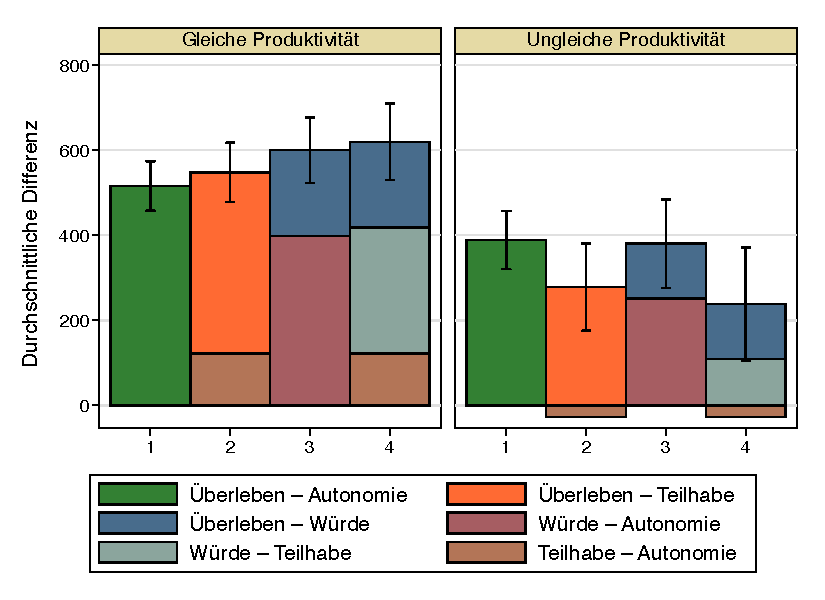
\includegraphics[width=0.99\linewidth]{figure_18.pdf}
\end{figure}

Im Anschluss an die Verantwortlichkeitsstudie (Abschnitt~\ref{sec:verantwortung}) sehen wir also auch in diesem Zusammenhang, dass das Leistungsprinzip im Denken unserer Teilnehmer*innen ebenso eine Rolle spielt wie das Bedarfsprinzip.
Die Bedeutung des Bedarfsprinzips, können wir jetzt sagen, bemisst sich außerdem an der Art des Bedarfs.
Wie viel Gewicht ihm für eine Verteilung beigemessen wird, hängt offensichtlich davon ab, als wie grundlegend der in Frage stehende Bedarf einer Person bewertet wird.


%%%%%%%%%%%%%%%%%%%
% ZUSAMMENFASSUNG %
%%%%%%%%%%%%%%%%%%%
\section{Zusammenfassung}\label{sec:zusammenfassung}
An dieser Stelle sollen die Hauptergebnisse unserer Studien noch einmal knapp zusammengefasst werden.
In Abschnitt~\ref{sec:referenzpunkt} wurde in den Blick genommen, ob es eine Verbindung gibt zwischen der Gerechtigkeitseinschätzung einer Situation und der in dieser Situation vorherrschenden Bedarfsdeckung.
Hierzu hatten die Teilnehmer*innen eine Reihe von Gerechtigkeitseinschätzungen zu verschiedenen Verteilungssituationen abzugeben, in denen sich die Güterversorgung sukzessive verbessert hat.
Dabei wurde ein Teil der Teilnehmer*innen außerdem über das Vorhandensein einer Bedarfsschwelle informiert, während der andere Teil keine zusätzlichen Informationen erhielt.
Wir haben beobachten können, dass die durchschnittlichen Gerechtigkeitseinschätzungen generell mit verbesserter Güterversorgung ansteigen, wobei die Bedarfsschwelle als ein Referenzpunkt für die Gerechtigkeitsbewertungen fungiert; das Erreichen der Schwelle führt zu einem sprunghaften Anstieg der wahrgenommenen Gerechtigkeit.

\begin{figure}[t]\label{fig:abbildung_19}
   \center
   \caption{Additivität für \enquote{Würde -- Autonomie} nach Szenario}
   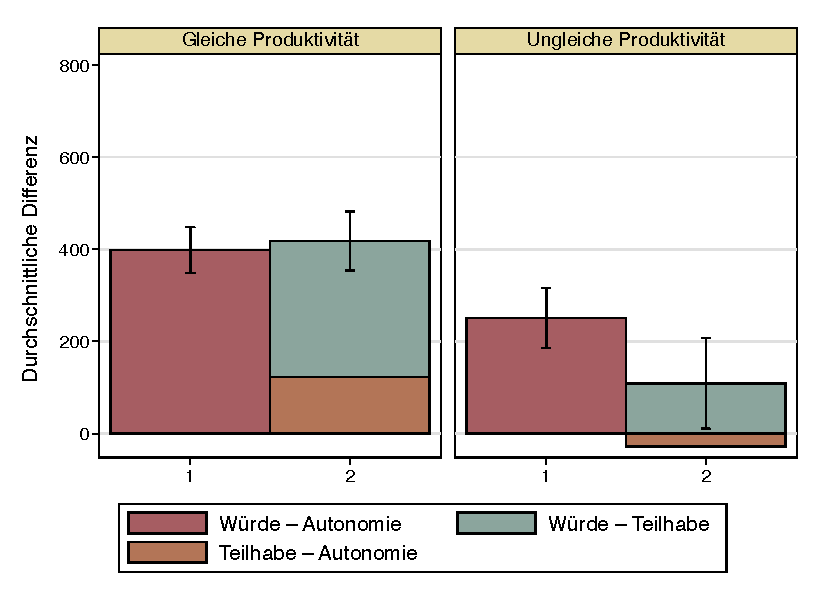
\includegraphics[width=0.99\linewidth]{figure_19.pdf}
\end{figure}

In Abschnitt~\ref{sec:verantwortung} wurde anschließend der Frage nachgegangen, ob neben solchen passiven Gerechtigkeitseinschätzungen auch aktive Verteilungsentscheidungen von Bedürfnissen beeinflusst werden.
Hierzu hatten die Teilnehmer*innen als unparteiische Entscheider*innen Verteilungsentscheidungen für zwei hypothetische Personen zu treffen, wobei sie deren Produktivität, Bedarf und Verantwortlichkeit zu berücksichtigen hatten.
Es hat sich gezeigt, dass der Bedarf der schlechtergestellten Person durchgehend zumindest anteilig kompensiert wird, wobei der Grad dieser Kompensation sinkt, wenn die Person für ihren Nachteil selbst verantwortlich ist.

In Abschnitt~\ref{sec:bedarfsarten} schließlich wurde in den Fokus genommen, welche Rolle unterschiedliche Bedarfsarten im Denken der Teilnehmer*innen spielen.
Hierzu wurden ihnen vier verschiedene Bedarfsarten präsentiert, die sie entweder hinsichtlich ihrer Wichtigkeit bewerten mussten (Abschnitt~\ref{sec:bedarfsarten_1}) oder die sie bei der Verteilung eines Gutes auf zwei hypothetische Personen zu berücksichtigen hatten (Abschnitt~\ref{sec:bedarfsarten_2}).
Es hat sich gezeigt, dass die Teilnehmer*innen den vier Bedarfsarten unterschiedliche Wichtigkeit zuschreiben, was sich auch in den Verteilungsentscheidungen widerspiegelt.
Am grundlegendsten ist die Kategorie Überleben, gefolgt von Würde, Teilhabe und Autonomie.
Wieder zeigt sich, dass die Verteilungsentscheidungen~-- neben der Bedarfsart~-- von der Leistung der Personen abhängen, dass die benachteiligte Person aber auch anteilig kompensiert wird.

Empirische Forschung wie die vorliegende wird durch eine Reihe von Faktoren eingeschränkt, prominenterweise etwa von Zeit und Budget.
Die oben dargestellte Forschung stellt vor diesem Hintergrund nur eine Auswahl der sinnvollen Herangehensweisen dar, mit denen man sich unserem Gegenstand annähern kann.
Außerdem ist sie das Ergebnis kooperativer Arbeiten und als solche immer das Ergebnis von langen Debatten, an deren Ende ein Konsens der beteiligten Forscher steht, der in aller Regel nicht alle vorgebrachten Ideen berücksichtigt.
An dieser Stelle soll daher in aller Kürze skizziert werden, welche Erweiterungen der vorliegenden Projekte ich für wünschenswert halte.

\begin{figure}[t]\label{fig:abbildung_20}
   \center
   \caption{Additivität für \enquote{Überleben -- Teilhabe} nach Szenario}
   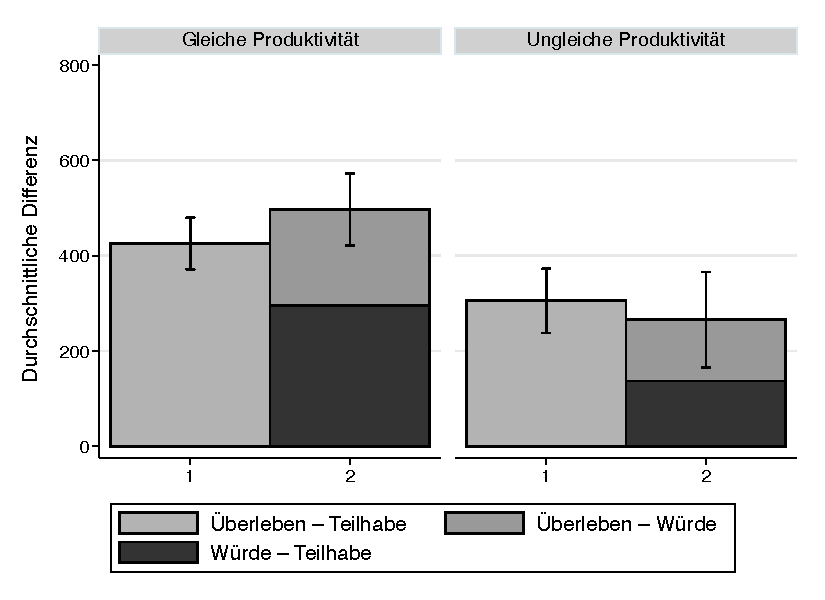
\includegraphics[width=0.99\linewidth]{figure_20.pdf}
\end{figure}

Die vorliegenden Studien beleuchten das Konzept des Bedarfs in erster Linie über Gerechtigkeitsbewertungen und Verteilungsentscheidungen.
Sie beleuchten den Gegenstand damit vorrangig aus einer quantitativen Perspektive.
Im Sinne eines Methodenmixes bin ich der Meinung, dass dem unbedingt Studien zum begrifflichen Konzept an die Seite gestellt werden sollten (wie etwa von \cite{poelzler_typicality_2022}).

Aber auch unsere quantitativen Studien lassen sich in vielerlei Hinsicht weiterdenken.
Unsere Vignetten beispielsweise beziehen sich durchgehend auf haushaltsbezogene Kontexte.
Im Sinne der externen Validität ließe sich hier über weitere Vignetten nachdenken, beispielsweise solche, denen unterschiedliche Sphären beziehungsweise soziale Zusammenhänge zugrunde liegen.

Ferner gibt es ganz konkrete Entscheidungen im Studienaufbau, die sich alternieren lassen.
Für die Referenzpunktstudie (Abschnitt~\ref{sec:referenzpunkt}), um nur ein Beispiel zu nennen, wäre es spannend, zu überprüfen, wie die Datenlage aussieht, wenn die einzelnen Szenarien nicht hintereinander, sondern in zufälliger Reihenfolge präsentiert werden.
Man könnte zudem überprüfen, wie die Ergebnisse aussehen, wenn die Teilnehmer*innen zufällige ganzzahlige Verteilungen erhalten, so dass wir ein feiner aufgelöstes Bild erhalten und~-- insbesondere in der Nähe zum Referenzpunkt~-- bessere Aussagen darüber treffen können, was zwischen unseren 11 Szenarien passiert. Außerdem halte ich eine Kontrollgruppe für sinnvoll, die statt gar keinen Referenzpunkt präsentiert zu bekommen, einen Referenzpunkt präsentiert bekommt, der ohne normative Bedeutung ist.

Es gibt also auch im Anschluss an diese Arbeit noch mehr als genug zu tun.


%%%%%%%%%%%%%%%%
% BIBLIOGRAFIE %
%%%%%%%%%%%%%%%%
\clearpage
\printbibliography[title={Bibliografie}]
\addcontentsline{toc}{section}{Bibliografie}


%%%%%%%%%%%%
% APPENDIX %
%%%%%%%%%%%%
\clearpage
\section*{Appendix}
\addcontentsline{toc}{section}{Appendix}
Auf den folgenden Seiten finden sich die der Dissertation zugrundeliegenden Arbeiten in nachstehender Reihenfolge:

\vspace{1em}
\noindent\hangindent=0.4cm Bauer, Alexander Max (2019a). \enquote{Gerechtigkeit und Bedürfnis. Perspektiven auf den Begriff des \enquote{Bedürfnisses} vor dem Hintergrund der Bedarfsgerechtigkeit}. In: \textit{Oldenburger Jahrbuch für Philosophie 2017/2018}. Hrsg. von Alexander Max Bauer und Nils Baratella. Oldenburg: BIS-Verlag, S.~285--327.

\noindent\hangindent=0.4cm Bauer, Alexander Max, Adele Diederich, Stefan Traub und Arne Robert Weiss (2023). \textit{When the Poorest Are Neglected. A Vignette Experiment on Need-Based Distributive Justice}. SSRN Working Paper 4503209. \textcolor{gray}{(eingereicht bei \textit{American Political Science Review})}

\noindent\hangindent=0.4cm Bauer, Alexander Max, Frauke Meyer, Jan Romann, Mark Siebel und Stefan Traub (2022a). \enquote{Need, Equity, and Accountability. Evidence on Third-Party Distributive Decisions from a Vignette Study}. In: \textit{Social Choice and Welfare} 59, S. 769--814.

\noindent\hangindent=0.4cm Bauer, Alexander Max und Malte Ingo Meyerhuber (2019b). \enquote{Zwei Welten am Rande der Kollision. Zum Verhältnis von empirischer Forschung und normativer Theorie, insbesondere vor dem Hintergrund der Ethik}. In: \textit{Philosophie zwischen Sein und Sollen. Normative Theorie und empirische Forschung im Spannungsfeld}. Hrsg. von Alexander Max Bauer und Malte Ingo Meyerhuber. Berlin und Boston: Walter de Gruyter, S.~13--37.

\noindent\hangindent=0.4cm Bauer, Alexander Max und Jan Romann (in Vorbereitung). \enquote{Equal Deeds, Different Needs. Need, Accountability, and Ressource Availability in Third-Party Distributive Decisions}. In: \textit{Oxford Studies in Experimental Philosophy}. Hrsg. von Shaun Nichols und Joshua Knobe. Oxford: Oxford University Press.

\noindent\hangindent=0.4cm Bauer, Alexander Max, Jan Romann, Mark Siebel und Stefan Traub (2023). \textit{Winter is Coming. How Laypeople Think About Different Kinds of Needs}. SSRN Working Paper 4383555. \textcolor{gray}{(in Überarbeitung für \textit{PLOS ONE})}

\noindent\hangindent=0.4cm Bauer, Alexander Max und Mark Siebel (in Vorbereitung). \enquote{Measuring Need-Based Distributive Justice -- Formally and Empirically}. In: \textit{Priority of Needs. An Informed Theory of Need-Based Justice}. Hrsg. von Stefan Traub und Bernhard Kittel. Cham: Springer.

\newpage\null\newpage

\includepdf[pages=-,frame=true,noautoscale=true,pagecommand={}]{publications/bauer_2019.pdf}\newpage\null\newpage
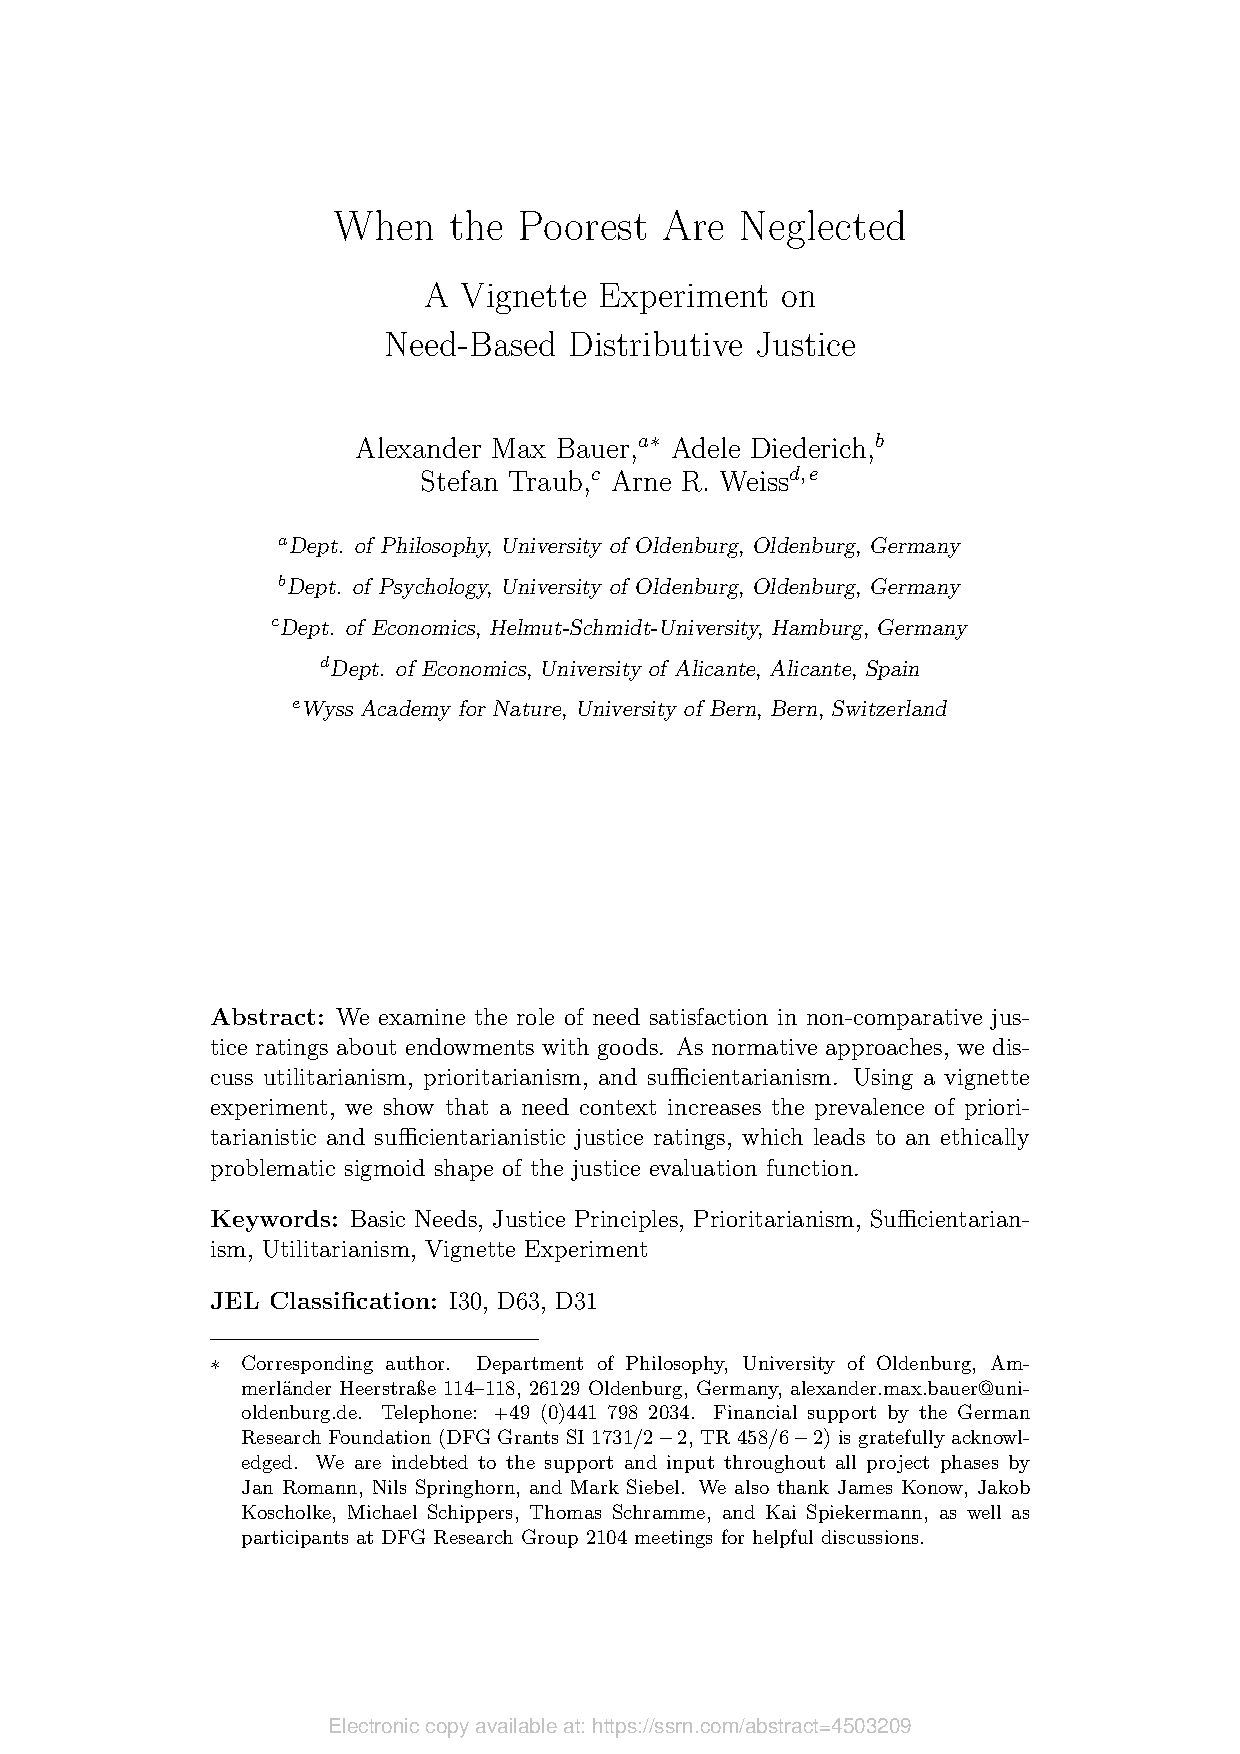
\includepdf[pages=-,frame=true,noautoscale=false,templatesize={500pt}{500pt},pagecommand={}]{publications/bauer_et_al_2023b.pdf}\newpage\null\newpage\newpage\null\newpage
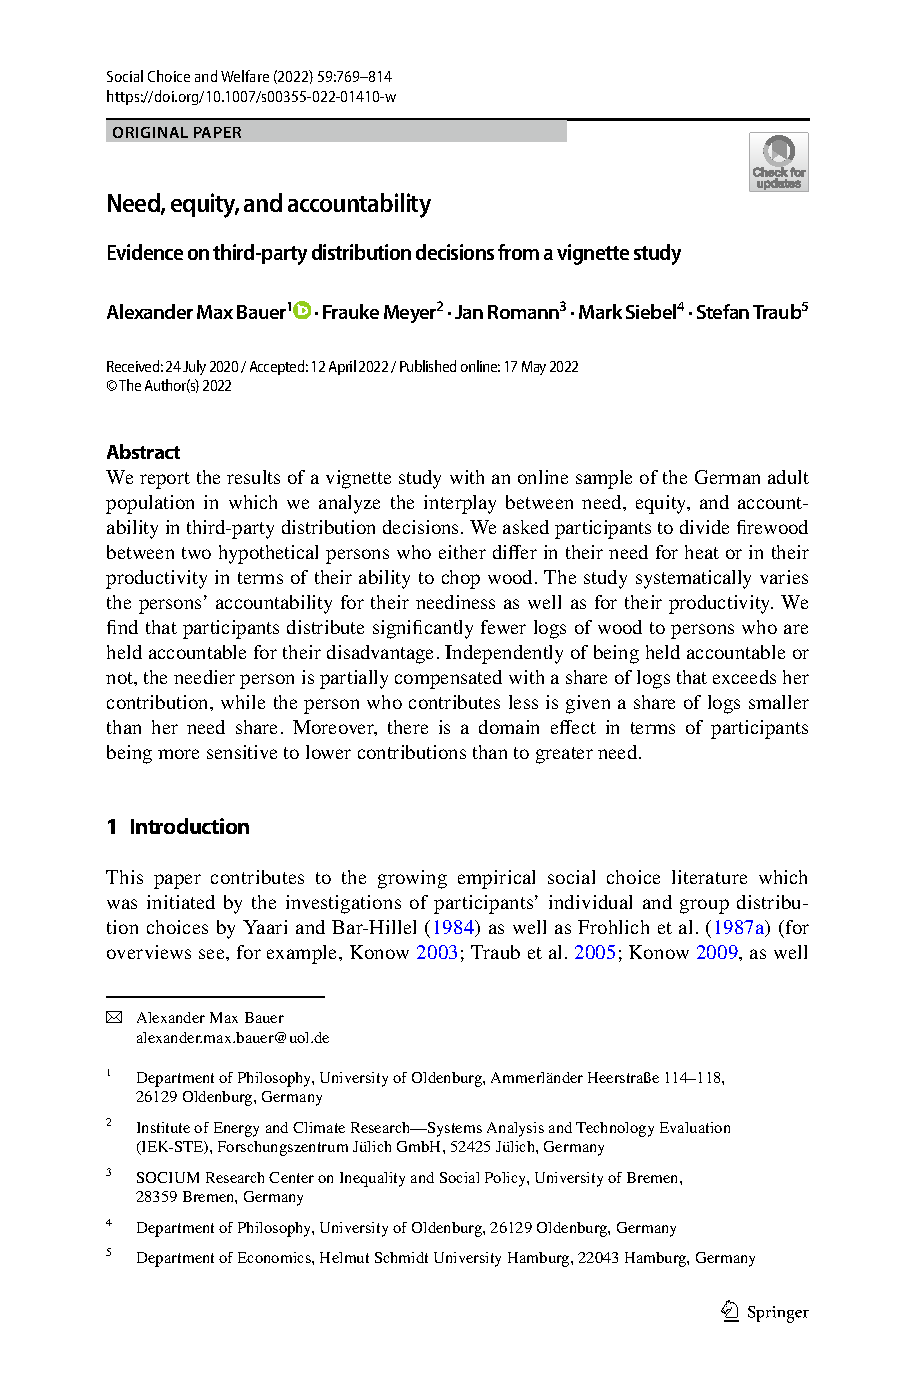
\includepdf[pages=-,frame=true,noautoscale=true,pagecommand={}]{publications/bauer_et_al_2022.pdf}\newpage\null\newpage
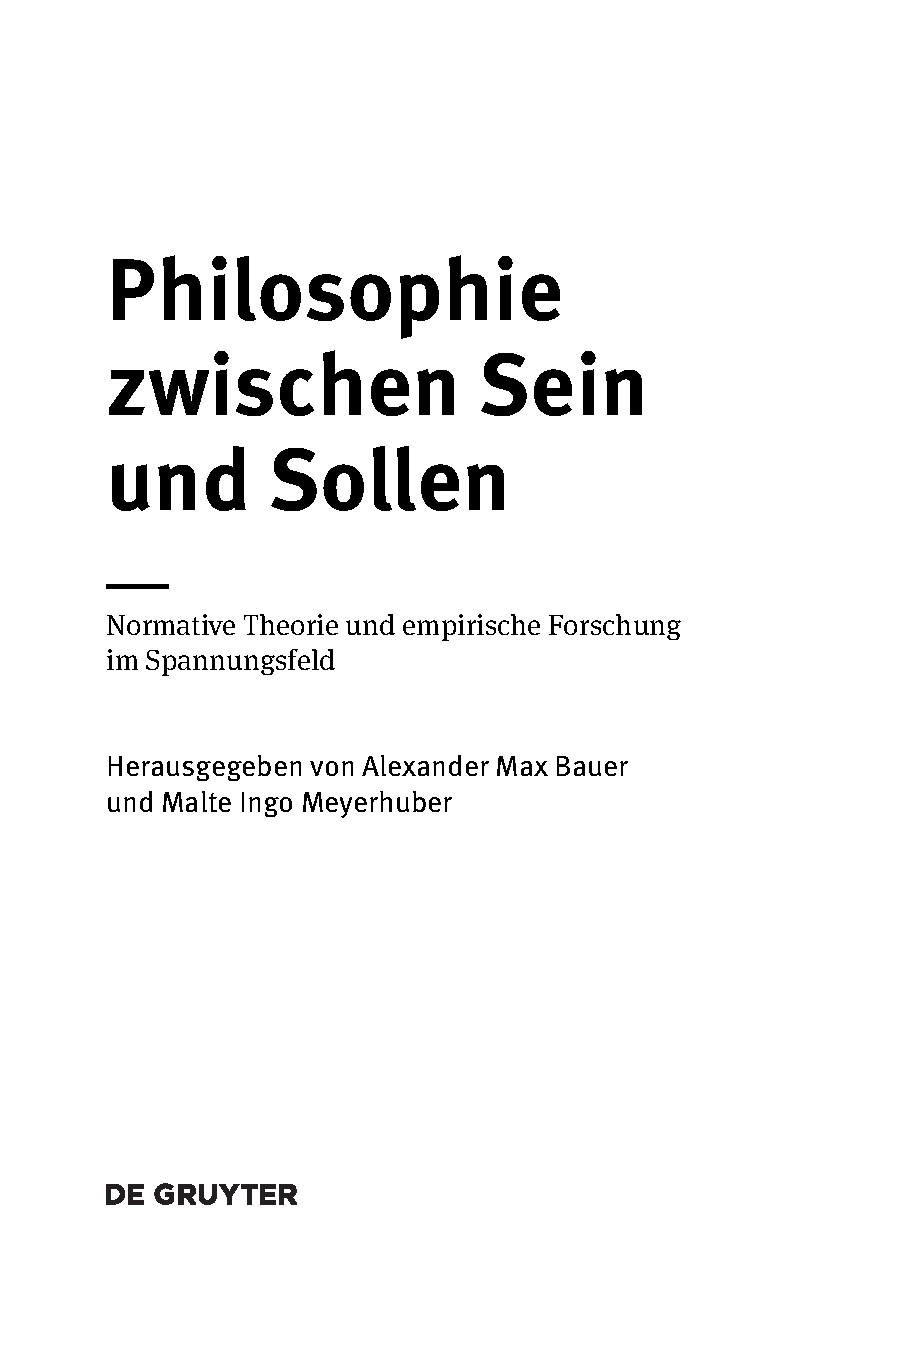
\includepdf[pages=-,frame=true,noautoscale=true,pagecommand={}]{publications/bauer_meyerhuber_2019.pdf}\newpage\null\newpage
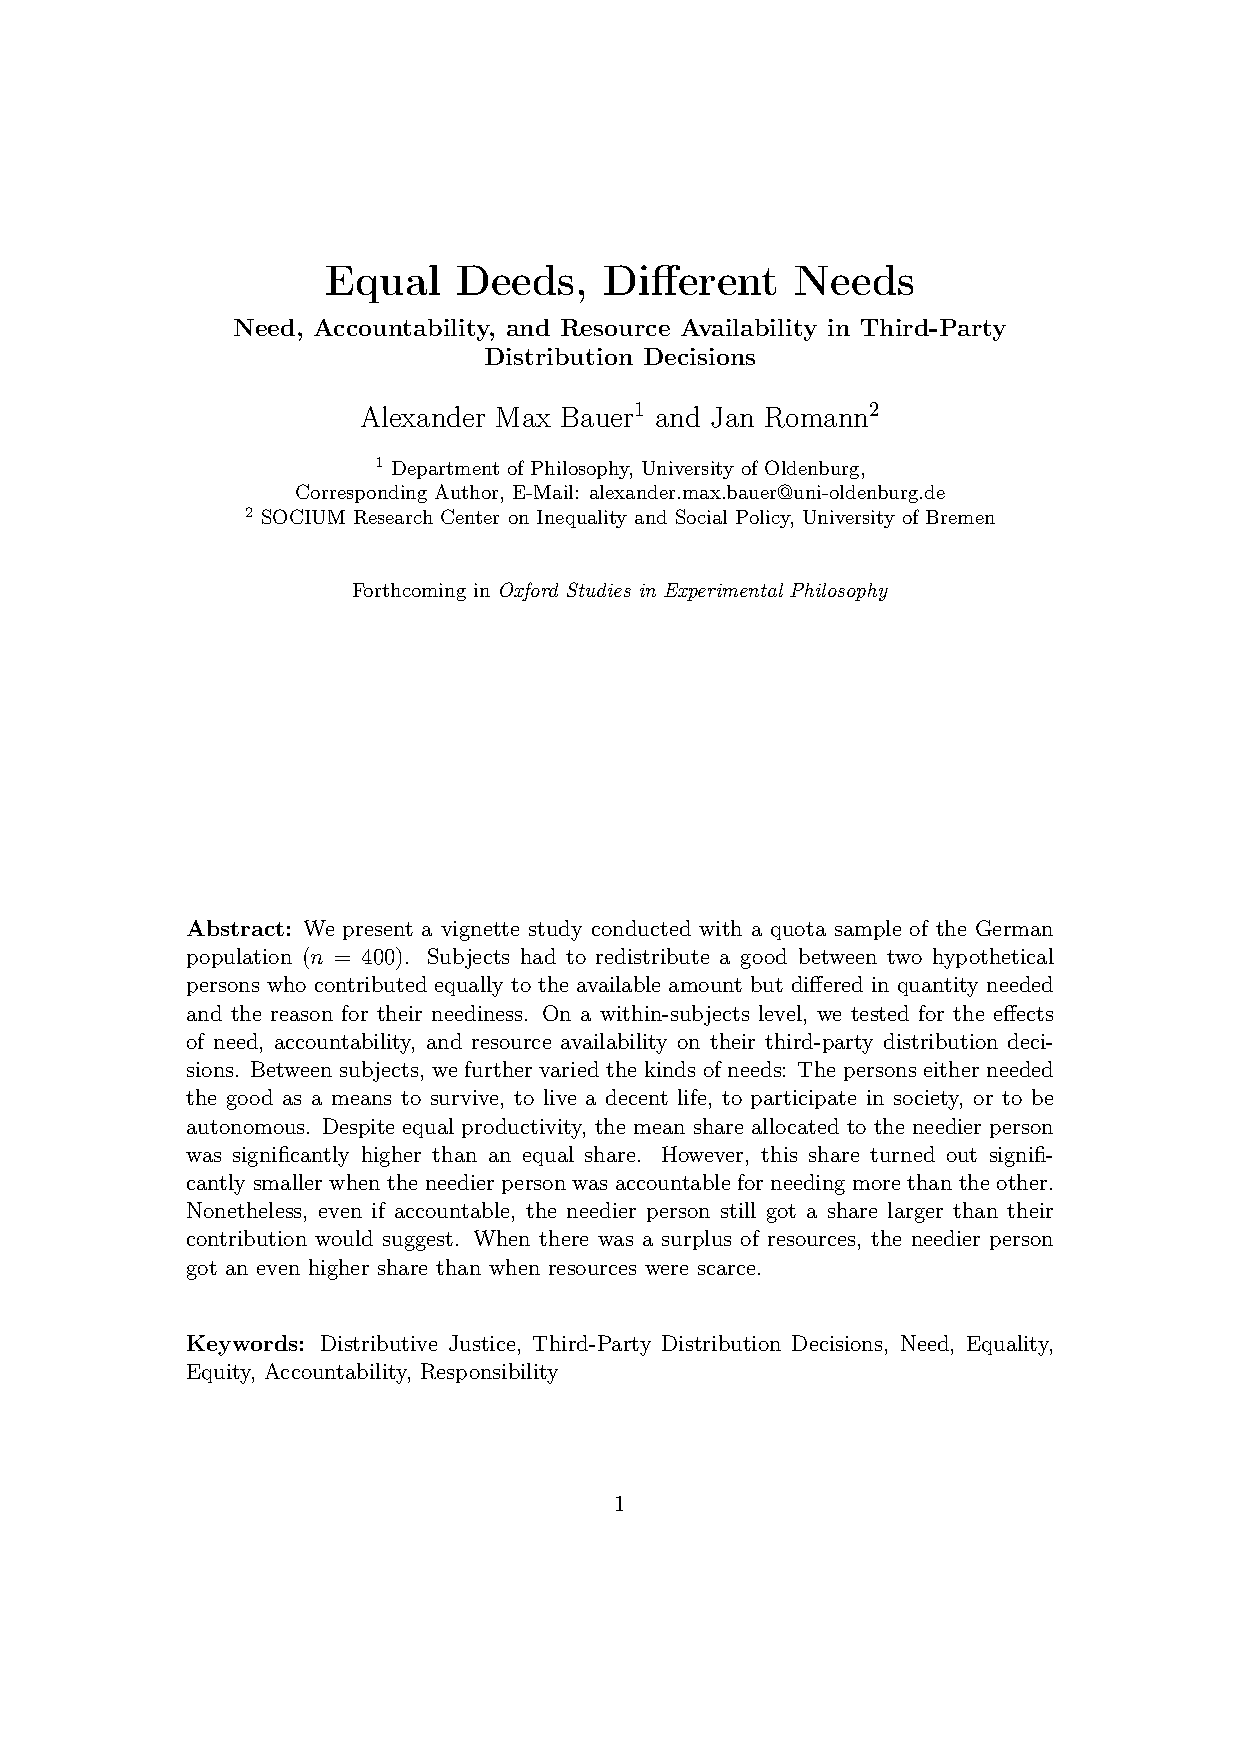
\includepdf[pages=-,frame=true,noautoscale=false,templatesize={500pt}{500pt},pagecommand={}]{publications/bauer_romann_nd.pdf}\newpage\null\newpage\newpage\null\newpage
\includepdf[pages=-,frame=true,noautoscale=false,templatesize={500pt}{500pt},pagecommand={}]{publications/bauer_et_al_2023a.pdf}\newpage\null\newpage\newpage\null\newpage
% 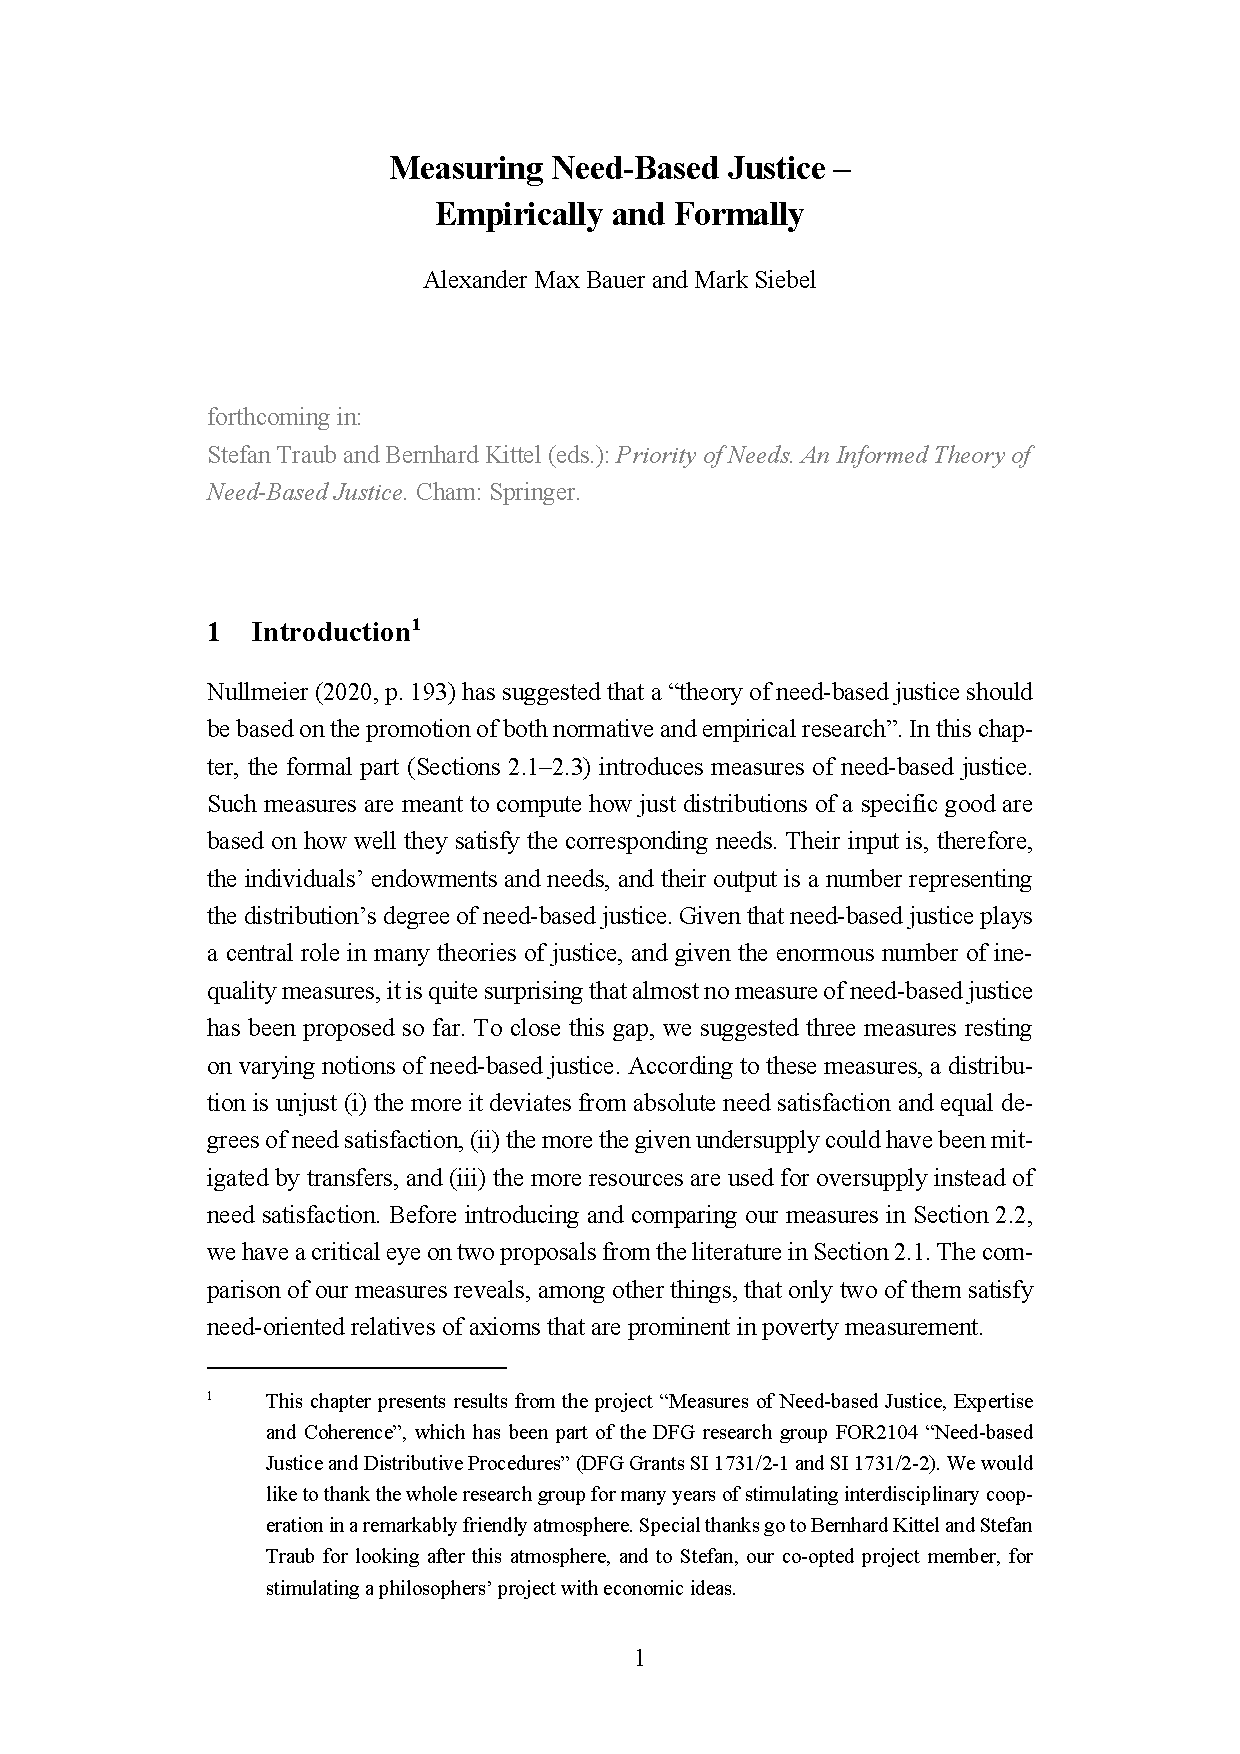
\includepdf[pages=-,frame=true,noautoscale=false,templatesize={500pt}{500pt},pagecommand={}]{publications/bauer_siebel_nd.pdf}


%%%%%%%%%%%%%
% ERKLÄRUNG %
%%%%%%%%%%%%%
\newpage\null\newpage
\section*{Erklärung}
\addcontentsline{toc}{section}{Erklärung}
Hiermit erkläre ich, dass ich die Dissertation selbständig verfasst, deren Inhalt nicht schon überwiegend für eine Diplom- oder vergleichbare Prüfungsarbeit verwendet habe und dass die benutzten Hilfsmittel vollständig angegeben sind.

Ferner erkläre ich, dass die Leitlinien guter wissenschaftlicher Praxis der Carl von Ossietzky Universität Oldenburg befolgt worden sind.

\vspace{3em}
\noindent Oldenburg, 12. Juli 2023\hspace{3em} Alexander Max Bauer

\end{document}
